\documentclass[twoside]{book}

% Packages required by doxygen
\usepackage{fixltx2e}
\usepackage{calc}
\usepackage{doxygen}
\usepackage[export]{adjustbox} % also loads graphicx
\usepackage{graphicx}
\usepackage[utf8]{inputenc}
\usepackage{makeidx}
\usepackage{multicol}
\usepackage{multirow}
\PassOptionsToPackage{warn}{textcomp}
\usepackage{textcomp}
\usepackage[nointegrals]{wasysym}
\usepackage[table]{xcolor}

% Font selection
\usepackage[T1]{fontenc}
\usepackage[scaled=.90]{helvet}
\usepackage{courier}
\usepackage{amssymb}
\usepackage{sectsty}
\renewcommand{\familydefault}{\sfdefault}
\allsectionsfont{%
  \fontseries{bc}\selectfont%
  \color{darkgray}%
}
\renewcommand{\DoxyLabelFont}{%
  \fontseries{bc}\selectfont%
  \color{darkgray}%
}
\newcommand{\+}{\discretionary{\mbox{\scriptsize$\hookleftarrow$}}{}{}}

% Page & text layout
\usepackage{geometry}
\geometry{%
  a4paper,%
  top=2.5cm,%
  bottom=2.5cm,%
  left=2.5cm,%
  right=2.5cm%
}
\tolerance=750
\hfuzz=15pt
\hbadness=750
\setlength{\emergencystretch}{15pt}
\setlength{\parindent}{0cm}
\setlength{\parskip}{0.2cm}
\makeatletter
\renewcommand{\paragraph}{%
  \@startsection{paragraph}{4}{0ex}{-1.0ex}{1.0ex}{%
    \normalfont\normalsize\bfseries\SS@parafont%
  }%
}
\renewcommand{\subparagraph}{%
  \@startsection{subparagraph}{5}{0ex}{-1.0ex}{1.0ex}{%
    \normalfont\normalsize\bfseries\SS@subparafont%
  }%
}
\makeatother

% Headers & footers
\usepackage{fancyhdr}
\pagestyle{fancyplain}
\fancyhead[LE]{\fancyplain{}{\bfseries\thepage}}
\fancyhead[CE]{\fancyplain{}{}}
\fancyhead[RE]{\fancyplain{}{\bfseries\leftmark}}
\fancyhead[LO]{\fancyplain{}{\bfseries\rightmark}}
\fancyhead[CO]{\fancyplain{}{}}
\fancyhead[RO]{\fancyplain{}{\bfseries\thepage}}
\fancyfoot[LE]{\fancyplain{}{}}
\fancyfoot[CE]{\fancyplain{}{}}
\fancyfoot[RE]{\fancyplain{}{\bfseries\scriptsize Generated on Tue Jun 9 2015 22\+:07\+:30 for Last Stand Engine by Doxygen }}
\fancyfoot[LO]{\fancyplain{}{\bfseries\scriptsize Generated on Tue Jun 9 2015 22\+:07\+:30 for Last Stand Engine by Doxygen }}
\fancyfoot[CO]{\fancyplain{}{}}
\fancyfoot[RO]{\fancyplain{}{}}
\renewcommand{\footrulewidth}{0.4pt}
\renewcommand{\chaptermark}[1]{%
  \markboth{#1}{}%
}
\renewcommand{\sectionmark}[1]{%
  \markright{\thesection\ #1}%
}

% Indices & bibliography
\usepackage{natbib}
\usepackage[titles]{tocloft}
\setcounter{tocdepth}{3}
\setcounter{secnumdepth}{5}
\makeindex

% Hyperlinks (required, but should be loaded last)
\usepackage{ifpdf}
\ifpdf
  \usepackage[pdftex,pagebackref=true]{hyperref}
\else
  \usepackage[ps2pdf,pagebackref=true]{hyperref}
\fi
\hypersetup{%
  colorlinks=true,%
  linkcolor=blue,%
  citecolor=blue,%
  unicode%
}

% Custom commands
\newcommand{\clearemptydoublepage}{%
  \newpage{\pagestyle{empty}\cleardoublepage}%
}


%===== C O N T E N T S =====

\begin{document}

% Titlepage & ToC
\hypersetup{pageanchor=false,
             bookmarks=true,
             bookmarksnumbered=true,
             pdfencoding=unicode
            }
\pagenumbering{roman}
\begin{titlepage}
\vspace*{7cm}
\begin{center}%
{\Large Last Stand Engine \\[1ex]\large 0 }\\
\vspace*{1cm}
{\large Generated by Doxygen 1.8.9.1}\\
\vspace*{0.5cm}
{\small Tue Jun 9 2015 22:07:30}\\
\end{center}
\end{titlepage}
\clearemptydoublepage
\tableofcontents
\clearemptydoublepage
\pagenumbering{arabic}
\hypersetup{pageanchor=true}

%--- Begin generated contents ---
\chapter{Hierarchical Index}
\section{Class Hierarchy}
This inheritance list is sorted roughly, but not completely, alphabetically\+:\begin{DoxyCompactList}
\item \contentsline{section}{File}{\pageref{classFile}}{}
\item \contentsline{section}{I\+Manages}{\pageref{classIManages}}{}
\begin{DoxyCompactList}
\item \contentsline{section}{Audio\+Manager}{\pageref{classAudioManager}}{}
\item \contentsline{section}{Input\+Manager}{\pageref{classInputManager}}{}
\item \contentsline{section}{Manager}{\pageref{classManager}}{}
\item \contentsline{section}{Network\+Manager}{\pageref{classNetworkManager}}{}
\end{DoxyCompactList}
\item \contentsline{section}{I\+Renderable2\+D}{\pageref{classIRenderable2D}}{}
\begin{DoxyCompactList}
\item \contentsline{section}{Actor2\+D}{\pageref{classActor2D}}{}
\end{DoxyCompactList}
\item \contentsline{section}{I\+Renderable3\+D}{\pageref{classIRenderable3D}}{}
\begin{DoxyCompactList}
\item \contentsline{section}{Actor3\+D}{\pageref{classActor3D}}{}
\end{DoxyCompactList}
\item \contentsline{section}{Log}{\pageref{classLog}}{}
\item \contentsline{section}{Math}{\pageref{classMath}}{}
\item \contentsline{section}{Matrix}{\pageref{classMatrix}}{}
\item \contentsline{section}{Plane}{\pageref{classPlane}}{}
\item \contentsline{section}{Quaternion}{\pageref{classQuaternion}}{}
\item \contentsline{section}{Universe}{\pageref{classUniverse}}{}
\item \contentsline{section}{Last\+Stand\+Engine\+:\+:Utils\+:\+:Utils}{\pageref{classLastStandEngine_1_1Utils_1_1Utils}}{}
\item \contentsline{section}{Vector2}{\pageref{structVector2}}{}
\item \contentsline{section}{Last\+Stand\+Engine\+:\+:Maths\+:\+:Vector4}{\pageref{structLastStandEngine_1_1Maths_1_1Vector4}}{}
\end{DoxyCompactList}

\chapter{Class Index}
\section{Class List}
Here are the classes, structs, unions and interfaces with brief descriptions\+:\begin{DoxyCompactList}
\item\contentsline{section}{\hyperlink{struct__SDLNet__GenericSocket}{\+\_\+\+S\+D\+L\+Net\+\_\+\+Generic\+Socket} }{\pageref{struct__SDLNet__GenericSocket}}{}
\item\contentsline{section}{\hyperlink{structAppProofOfPurchaseKeyResponse__t}{App\+Proof\+Of\+Purchase\+Key\+Response\+\_\+t} }{\pageref{structAppProofOfPurchaseKeyResponse__t}}{}
\item\contentsline{section}{\hyperlink{structValve_1_1Steamworks_1_1AppProofOfPurchaseKeyResponse__t}{Valve.\+Steamworks.\+App\+Proof\+Of\+Purchase\+Key\+Response\+\_\+t} }{\pageref{structValve_1_1Steamworks_1_1AppProofOfPurchaseKeyResponse__t}}{}
\item\contentsline{section}{\hyperlink{structAssociateWithClanResult__t}{Associate\+With\+Clan\+Result\+\_\+t} }{\pageref{structAssociateWithClanResult__t}}{}
\item\contentsline{section}{\hyperlink{structValve_1_1Steamworks_1_1AssociateWithClanResult__t}{Valve.\+Steamworks.\+Associate\+With\+Clan\+Result\+\_\+t} }{\pageref{structValve_1_1Steamworks_1_1AssociateWithClanResult__t}}{}
\item\contentsline{section}{\hyperlink{structValve_1_1Steamworks_1_1AvatarImageLoaded__t}{Valve.\+Steamworks.\+Avatar\+Image\+Loaded\+\_\+t} }{\pageref{structValve_1_1Steamworks_1_1AvatarImageLoaded__t}}{}
\item\contentsline{section}{\hyperlink{structAvatarImageLoaded__t}{Avatar\+Image\+Loaded\+\_\+t} }{\pageref{structAvatarImageLoaded__t}}{}
\item\contentsline{section}{\hyperlink{structValve_1_1Steamworks_1_1BroadcastUploadStop__t}{Valve.\+Steamworks.\+Broadcast\+Upload\+Stop\+\_\+t} }{\pageref{structValve_1_1Steamworks_1_1BroadcastUploadStop__t}}{}
\item\contentsline{section}{\hyperlink{structValve_1_1Steamworks_1_1CallbackMsg__t}{Valve.\+Steamworks.\+Callback\+Msg\+\_\+t} }{\pageref{structValve_1_1Steamworks_1_1CallbackMsg__t}}{}
\item\contentsline{section}{\hyperlink{structCallbackMsg__t}{Callback\+Msg\+\_\+t} }{\pageref{structCallbackMsg__t}}{}
\item\contentsline{section}{\hyperlink{classCCallback}{C\+Callback$<$ T, P, b\+Game\+Server $>$} }{\pageref{classCCallback}}{}
\item\contentsline{section}{\hyperlink{structValve_1_1Steamworks_1_1CCallback}{Valve.\+Steamworks.\+C\+Callback} }{\pageref{structValve_1_1Steamworks_1_1CCallback}}{}
\item\contentsline{section}{\hyperlink{classCCallbackBase}{C\+Callback\+Base} }{\pageref{classCCallbackBase}}{}
\item\contentsline{section}{\hyperlink{structValve_1_1Steamworks_1_1CCallbackBase}{Valve.\+Steamworks.\+C\+Callback\+Base} }{\pageref{structValve_1_1Steamworks_1_1CCallbackBase}}{}
\item\contentsline{section}{\hyperlink{classCCallbackManual}{C\+Callback\+Manual$<$ T, P, b\+Game\+Server $>$} }{\pageref{classCCallbackManual}}{}
\item\contentsline{section}{\hyperlink{classCCallResult}{C\+Call\+Result$<$ T, P $>$} }{\pageref{classCCallResult}}{}
\item\contentsline{section}{\hyperlink{structValve_1_1Steamworks_1_1CCallResult}{Valve.\+Steamworks.\+C\+Call\+Result} }{\pageref{structValve_1_1Steamworks_1_1CCallResult}}{}
\item\contentsline{section}{\hyperlink{classCGameID}{C\+Game\+I\+D} }{\pageref{classCGameID}}{}
\item\contentsline{section}{\hyperlink{structValve_1_1Steamworks_1_1CheckFileSignature__t}{Valve.\+Steamworks.\+Check\+File\+Signature\+\_\+t} }{\pageref{structValve_1_1Steamworks_1_1CheckFileSignature__t}}{}
\item\contentsline{section}{\hyperlink{structCheckFileSignature__t}{Check\+File\+Signature\+\_\+t} }{\pageref{structCheckFileSignature__t}}{}
\item\contentsline{section}{\hyperlink{structValve_1_1Steamworks_1_1ClanOfficerListResponse__t}{Valve.\+Steamworks.\+Clan\+Officer\+List\+Response\+\_\+t} }{\pageref{structValve_1_1Steamworks_1_1ClanOfficerListResponse__t}}{}
\item\contentsline{section}{\hyperlink{structClanOfficerListResponse__t}{Clan\+Officer\+List\+Response\+\_\+t} }{\pageref{structClanOfficerListResponse__t}}{}
\item\contentsline{section}{\hyperlink{structValve_1_1Steamworks_1_1ClientGameServerDeny__t}{Valve.\+Steamworks.\+Client\+Game\+Server\+Deny\+\_\+t} }{\pageref{structValve_1_1Steamworks_1_1ClientGameServerDeny__t}}{}
\item\contentsline{section}{\hyperlink{structClientGameServerDeny__t}{Client\+Game\+Server\+Deny\+\_\+t} }{\pageref{structClientGameServerDeny__t}}{}
\item\contentsline{section}{\hyperlink{structComputeNewPlayerCompatibilityResult__t}{Compute\+New\+Player\+Compatibility\+Result\+\_\+t} }{\pageref{structComputeNewPlayerCompatibilityResult__t}}{}
\item\contentsline{section}{\hyperlink{structValve_1_1Steamworks_1_1ComputeNewPlayerCompatibilityResult__t}{Valve.\+Steamworks.\+Compute\+New\+Player\+Compatibility\+Result\+\_\+t} }{\pageref{structValve_1_1Steamworks_1_1ComputeNewPlayerCompatibilityResult__t}}{}
\item\contentsline{section}{\hyperlink{structCreateItemResult__t}{Create\+Item\+Result\+\_\+t} }{\pageref{structCreateItemResult__t}}{}
\item\contentsline{section}{\hyperlink{structValve_1_1Steamworks_1_1CreateItemResult__t}{Valve.\+Steamworks.\+Create\+Item\+Result\+\_\+t} }{\pageref{structValve_1_1Steamworks_1_1CreateItemResult__t}}{}
\item\contentsline{section}{\hyperlink{structValve_1_1Steamworks_1_1CSteamAPIContext}{Valve.\+Steamworks.\+C\+Steam\+A\+P\+I\+Context} }{\pageref{structValve_1_1Steamworks_1_1CSteamAPIContext}}{}
\item\contentsline{section}{\hyperlink{classValve_1_1Steamworks_1_1CSteamAppList}{Valve.\+Steamworks.\+C\+Steam\+App\+List} }{\pageref{classValve_1_1Steamworks_1_1CSteamAppList}}{}
\item\contentsline{section}{\hyperlink{classValve_1_1Steamworks_1_1CSteamApps}{Valve.\+Steamworks.\+C\+Steam\+Apps} }{\pageref{classValve_1_1Steamworks_1_1CSteamApps}}{}
\item\contentsline{section}{\hyperlink{classValve_1_1Steamworks_1_1CSteamClient}{Valve.\+Steamworks.\+C\+Steam\+Client} }{\pageref{classValve_1_1Steamworks_1_1CSteamClient}}{}
\item\contentsline{section}{\hyperlink{classValve_1_1Steamworks_1_1CSteamController}{Valve.\+Steamworks.\+C\+Steam\+Controller} }{\pageref{classValve_1_1Steamworks_1_1CSteamController}}{}
\item\contentsline{section}{\hyperlink{classValve_1_1Steamworks_1_1CSteamFriends}{Valve.\+Steamworks.\+C\+Steam\+Friends} }{\pageref{classValve_1_1Steamworks_1_1CSteamFriends}}{}
\item\contentsline{section}{\hyperlink{classValve_1_1Steamworks_1_1CSteamGameServer}{Valve.\+Steamworks.\+C\+Steam\+Game\+Server} }{\pageref{classValve_1_1Steamworks_1_1CSteamGameServer}}{}
\item\contentsline{section}{\hyperlink{classValve_1_1Steamworks_1_1CSteamGameServerStats}{Valve.\+Steamworks.\+C\+Steam\+Game\+Server\+Stats} }{\pageref{classValve_1_1Steamworks_1_1CSteamGameServerStats}}{}
\item\contentsline{section}{\hyperlink{classValve_1_1Steamworks_1_1CSteamHTMLSurface}{Valve.\+Steamworks.\+C\+Steam\+H\+T\+M\+L\+Surface} }{\pageref{classValve_1_1Steamworks_1_1CSteamHTMLSurface}}{}
\item\contentsline{section}{\hyperlink{classValve_1_1Steamworks_1_1CSteamHTTP}{Valve.\+Steamworks.\+C\+Steam\+H\+T\+T\+P} }{\pageref{classValve_1_1Steamworks_1_1CSteamHTTP}}{}
\item\contentsline{section}{\hyperlink{structValve_1_1Steamworks_1_1CSteamID}{Valve.\+Steamworks.\+C\+Steam\+I\+D} }{\pageref{structValve_1_1Steamworks_1_1CSteamID}}{}
\item\contentsline{section}{\hyperlink{classCSteamID}{C\+Steam\+I\+D} }{\pageref{classCSteamID}}{}
\item\contentsline{section}{\hyperlink{classValve_1_1Steamworks_1_1CSteamInventory}{Valve.\+Steamworks.\+C\+Steam\+Inventory} }{\pageref{classValve_1_1Steamworks_1_1CSteamInventory}}{}
\item\contentsline{section}{\hyperlink{classValve_1_1Steamworks_1_1CSteamMatchmaking}{Valve.\+Steamworks.\+C\+Steam\+Matchmaking} }{\pageref{classValve_1_1Steamworks_1_1CSteamMatchmaking}}{}
\item\contentsline{section}{\hyperlink{classValve_1_1Steamworks_1_1CSteamMatchmakingPingResponse}{Valve.\+Steamworks.\+C\+Steam\+Matchmaking\+Ping\+Response} }{\pageref{classValve_1_1Steamworks_1_1CSteamMatchmakingPingResponse}}{}
\item\contentsline{section}{\hyperlink{classValve_1_1Steamworks_1_1CSteamMatchmakingPlayersResponse}{Valve.\+Steamworks.\+C\+Steam\+Matchmaking\+Players\+Response} }{\pageref{classValve_1_1Steamworks_1_1CSteamMatchmakingPlayersResponse}}{}
\item\contentsline{section}{\hyperlink{classValve_1_1Steamworks_1_1CSteamMatchmakingRulesResponse}{Valve.\+Steamworks.\+C\+Steam\+Matchmaking\+Rules\+Response} }{\pageref{classValve_1_1Steamworks_1_1CSteamMatchmakingRulesResponse}}{}
\item\contentsline{section}{\hyperlink{classValve_1_1Steamworks_1_1CSteamMatchmakingServerListResponse}{Valve.\+Steamworks.\+C\+Steam\+Matchmaking\+Server\+List\+Response} }{\pageref{classValve_1_1Steamworks_1_1CSteamMatchmakingServerListResponse}}{}
\item\contentsline{section}{\hyperlink{classValve_1_1Steamworks_1_1CSteamMatchmakingServers}{Valve.\+Steamworks.\+C\+Steam\+Matchmaking\+Servers} }{\pageref{classValve_1_1Steamworks_1_1CSteamMatchmakingServers}}{}
\item\contentsline{section}{\hyperlink{classValve_1_1Steamworks_1_1CSteamMusic}{Valve.\+Steamworks.\+C\+Steam\+Music} }{\pageref{classValve_1_1Steamworks_1_1CSteamMusic}}{}
\item\contentsline{section}{\hyperlink{classValve_1_1Steamworks_1_1CSteamMusicRemote}{Valve.\+Steamworks.\+C\+Steam\+Music\+Remote} }{\pageref{classValve_1_1Steamworks_1_1CSteamMusicRemote}}{}
\item\contentsline{section}{\hyperlink{classValve_1_1Steamworks_1_1CSteamNetworking}{Valve.\+Steamworks.\+C\+Steam\+Networking} }{\pageref{classValve_1_1Steamworks_1_1CSteamNetworking}}{}
\item\contentsline{section}{\hyperlink{classValve_1_1Steamworks_1_1CSteamRemoteStorage}{Valve.\+Steamworks.\+C\+Steam\+Remote\+Storage} }{\pageref{classValve_1_1Steamworks_1_1CSteamRemoteStorage}}{}
\item\contentsline{section}{\hyperlink{classValve_1_1Steamworks_1_1CSteamScreenshots}{Valve.\+Steamworks.\+C\+Steam\+Screenshots} }{\pageref{classValve_1_1Steamworks_1_1CSteamScreenshots}}{}
\item\contentsline{section}{\hyperlink{classValve_1_1Steamworks_1_1CSteamUGC}{Valve.\+Steamworks.\+C\+Steam\+U\+G\+C} }{\pageref{classValve_1_1Steamworks_1_1CSteamUGC}}{}
\item\contentsline{section}{\hyperlink{classValve_1_1Steamworks_1_1CSteamUnifiedMessages}{Valve.\+Steamworks.\+C\+Steam\+Unified\+Messages} }{\pageref{classValve_1_1Steamworks_1_1CSteamUnifiedMessages}}{}
\item\contentsline{section}{\hyperlink{classValve_1_1Steamworks_1_1CSteamUser}{Valve.\+Steamworks.\+C\+Steam\+User} }{\pageref{classValve_1_1Steamworks_1_1CSteamUser}}{}
\item\contentsline{section}{\hyperlink{classValve_1_1Steamworks_1_1CSteamUserStats}{Valve.\+Steamworks.\+C\+Steam\+User\+Stats} }{\pageref{classValve_1_1Steamworks_1_1CSteamUserStats}}{}
\item\contentsline{section}{\hyperlink{classValve_1_1Steamworks_1_1CSteamUtils}{Valve.\+Steamworks.\+C\+Steam\+Utils} }{\pageref{classValve_1_1Steamworks_1_1CSteamUtils}}{}
\item\contentsline{section}{\hyperlink{classValve_1_1Steamworks_1_1CSteamVideo}{Valve.\+Steamworks.\+C\+Steam\+Video} }{\pageref{classValve_1_1Steamworks_1_1CSteamVideo}}{}
\item\contentsline{section}{\hyperlink{structDlcInstalled__t}{Dlc\+Installed\+\_\+t} }{\pageref{structDlcInstalled__t}}{}
\item\contentsline{section}{\hyperlink{structValve_1_1Steamworks_1_1DlcInstalled__t}{Valve.\+Steamworks.\+Dlc\+Installed\+\_\+t} }{\pageref{structValve_1_1Steamworks_1_1DlcInstalled__t}}{}
\item\contentsline{section}{\hyperlink{structValve_1_1Steamworks_1_1DownloadClanActivityCountsResult__t}{Valve.\+Steamworks.\+Download\+Clan\+Activity\+Counts\+Result\+\_\+t} }{\pageref{structValve_1_1Steamworks_1_1DownloadClanActivityCountsResult__t}}{}
\item\contentsline{section}{\hyperlink{structDownloadClanActivityCountsResult__t}{Download\+Clan\+Activity\+Counts\+Result\+\_\+t} }{\pageref{structDownloadClanActivityCountsResult__t}}{}
\item\contentsline{section}{\hyperlink{structDownloadItemResult__t}{Download\+Item\+Result\+\_\+t} }{\pageref{structDownloadItemResult__t}}{}
\item\contentsline{section}{\hyperlink{structValve_1_1Steamworks_1_1DownloadItemResult__t}{Valve.\+Steamworks.\+Download\+Item\+Result\+\_\+t} }{\pageref{structValve_1_1Steamworks_1_1DownloadItemResult__t}}{}
\item\contentsline{section}{\hyperlink{structValve_1_1Steamworks_1_1EncryptedAppTicketResponse__t}{Valve.\+Steamworks.\+Encrypted\+App\+Ticket\+Response\+\_\+t} }{\pageref{structValve_1_1Steamworks_1_1EncryptedAppTicketResponse__t}}{}
\item\contentsline{section}{\hyperlink{structEncryptedAppTicketResponse__t}{Encrypted\+App\+Ticket\+Response\+\_\+t} }{\pageref{structEncryptedAppTicketResponse__t}}{}
\item\contentsline{section}{\hyperlink{classEngine}{Engine} }{\pageref{classEngine}}{}
\item\contentsline{section}{\hyperlink{structFavoritesListAccountsUpdated__t}{Favorites\+List\+Accounts\+Updated\+\_\+t} }{\pageref{structFavoritesListAccountsUpdated__t}}{}
\item\contentsline{section}{\hyperlink{structValve_1_1Steamworks_1_1FavoritesListAccountsUpdated__t}{Valve.\+Steamworks.\+Favorites\+List\+Accounts\+Updated\+\_\+t} }{\pageref{structValve_1_1Steamworks_1_1FavoritesListAccountsUpdated__t}}{}
\item\contentsline{section}{\hyperlink{structFavoritesListChanged__t}{Favorites\+List\+Changed\+\_\+t} }{\pageref{structFavoritesListChanged__t}}{}
\item\contentsline{section}{\hyperlink{structValve_1_1Steamworks_1_1FavoritesListChanged__t}{Valve.\+Steamworks.\+Favorites\+List\+Changed\+\_\+t} }{\pageref{structValve_1_1Steamworks_1_1FavoritesListChanged__t}}{}
\item\contentsline{section}{\hyperlink{structValve_1_1Steamworks_1_1FriendGameInfo__t}{Valve.\+Steamworks.\+Friend\+Game\+Info\+\_\+t} }{\pageref{structValve_1_1Steamworks_1_1FriendGameInfo__t}}{}
\item\contentsline{section}{\hyperlink{structFriendGameInfo__t}{Friend\+Game\+Info\+\_\+t} }{\pageref{structFriendGameInfo__t}}{}
\item\contentsline{section}{\hyperlink{structValve_1_1Steamworks_1_1FriendRichPresenceUpdate__t}{Valve.\+Steamworks.\+Friend\+Rich\+Presence\+Update\+\_\+t} }{\pageref{structValve_1_1Steamworks_1_1FriendRichPresenceUpdate__t}}{}
\item\contentsline{section}{\hyperlink{structFriendRichPresenceUpdate__t}{Friend\+Rich\+Presence\+Update\+\_\+t} }{\pageref{structFriendRichPresenceUpdate__t}}{}
\item\contentsline{section}{\hyperlink{structValve_1_1Steamworks_1_1FriendsEnumerateFollowingList__t}{Valve.\+Steamworks.\+Friends\+Enumerate\+Following\+List\+\_\+t} }{\pageref{structValve_1_1Steamworks_1_1FriendsEnumerateFollowingList__t}}{}
\item\contentsline{section}{\hyperlink{structFriendsEnumerateFollowingList__t}{Friends\+Enumerate\+Following\+List\+\_\+t} }{\pageref{structFriendsEnumerateFollowingList__t}}{}
\item\contentsline{section}{\hyperlink{structValve_1_1Steamworks_1_1FriendSessionStateInfo__t}{Valve.\+Steamworks.\+Friend\+Session\+State\+Info\+\_\+t} }{\pageref{structValve_1_1Steamworks_1_1FriendSessionStateInfo__t}}{}
\item\contentsline{section}{\hyperlink{structFriendSessionStateInfo__t}{Friend\+Session\+State\+Info\+\_\+t} }{\pageref{structFriendSessionStateInfo__t}}{}
\item\contentsline{section}{\hyperlink{structValve_1_1Steamworks_1_1FriendsGetFollowerCount__t}{Valve.\+Steamworks.\+Friends\+Get\+Follower\+Count\+\_\+t} }{\pageref{structValve_1_1Steamworks_1_1FriendsGetFollowerCount__t}}{}
\item\contentsline{section}{\hyperlink{structFriendsGetFollowerCount__t}{Friends\+Get\+Follower\+Count\+\_\+t} }{\pageref{structFriendsGetFollowerCount__t}}{}
\item\contentsline{section}{\hyperlink{structValve_1_1Steamworks_1_1FriendsIsFollowing__t}{Valve.\+Steamworks.\+Friends\+Is\+Following\+\_\+t} }{\pageref{structValve_1_1Steamworks_1_1FriendsIsFollowing__t}}{}
\item\contentsline{section}{\hyperlink{structFriendsIsFollowing__t}{Friends\+Is\+Following\+\_\+t} }{\pageref{structFriendsIsFollowing__t}}{}
\item\contentsline{section}{\hyperlink{structValve_1_1Steamworks_1_1GameConnectedChatJoin__t}{Valve.\+Steamworks.\+Game\+Connected\+Chat\+Join\+\_\+t} }{\pageref{structValve_1_1Steamworks_1_1GameConnectedChatJoin__t}}{}
\item\contentsline{section}{\hyperlink{structGameConnectedChatJoin__t}{Game\+Connected\+Chat\+Join\+\_\+t} }{\pageref{structGameConnectedChatJoin__t}}{}
\item\contentsline{section}{\hyperlink{structValve_1_1Steamworks_1_1GameConnectedChatLeave__t}{Valve.\+Steamworks.\+Game\+Connected\+Chat\+Leave\+\_\+t} }{\pageref{structValve_1_1Steamworks_1_1GameConnectedChatLeave__t}}{}
\item\contentsline{section}{\hyperlink{structGameConnectedChatLeave__t}{Game\+Connected\+Chat\+Leave\+\_\+t} }{\pageref{structGameConnectedChatLeave__t}}{}
\item\contentsline{section}{\hyperlink{structValve_1_1Steamworks_1_1GameConnectedClanChatMsg__t}{Valve.\+Steamworks.\+Game\+Connected\+Clan\+Chat\+Msg\+\_\+t} }{\pageref{structValve_1_1Steamworks_1_1GameConnectedClanChatMsg__t}}{}
\item\contentsline{section}{\hyperlink{structGameConnectedClanChatMsg__t}{Game\+Connected\+Clan\+Chat\+Msg\+\_\+t} }{\pageref{structGameConnectedClanChatMsg__t}}{}
\item\contentsline{section}{\hyperlink{structValve_1_1Steamworks_1_1GameConnectedFriendChatMsg__t}{Valve.\+Steamworks.\+Game\+Connected\+Friend\+Chat\+Msg\+\_\+t} }{\pageref{structValve_1_1Steamworks_1_1GameConnectedFriendChatMsg__t}}{}
\item\contentsline{section}{\hyperlink{structGameConnectedFriendChatMsg__t}{Game\+Connected\+Friend\+Chat\+Msg\+\_\+t} }{\pageref{structGameConnectedFriendChatMsg__t}}{}
\item\contentsline{section}{\hyperlink{structValve_1_1Steamworks_1_1GameID__t}{Valve.\+Steamworks.\+Game\+I\+D\+\_\+t} }{\pageref{structValve_1_1Steamworks_1_1GameID__t}}{}
\item\contentsline{section}{\hyperlink{structValve_1_1Steamworks_1_1GameLobbyJoinRequested__t}{Valve.\+Steamworks.\+Game\+Lobby\+Join\+Requested\+\_\+t} }{\pageref{structValve_1_1Steamworks_1_1GameLobbyJoinRequested__t}}{}
\item\contentsline{section}{\hyperlink{structGameLobbyJoinRequested__t}{Game\+Lobby\+Join\+Requested\+\_\+t} }{\pageref{structGameLobbyJoinRequested__t}}{}
\item\contentsline{section}{\hyperlink{structValve_1_1Steamworks_1_1GameOverlayActivated__t}{Valve.\+Steamworks.\+Game\+Overlay\+Activated\+\_\+t} }{\pageref{structValve_1_1Steamworks_1_1GameOverlayActivated__t}}{}
\item\contentsline{section}{\hyperlink{structGameOverlayActivated__t}{Game\+Overlay\+Activated\+\_\+t} }{\pageref{structGameOverlayActivated__t}}{}
\item\contentsline{section}{\hyperlink{structValve_1_1Steamworks_1_1GamepadTextInputDismissed__t}{Valve.\+Steamworks.\+Gamepad\+Text\+Input\+Dismissed\+\_\+t} }{\pageref{structValve_1_1Steamworks_1_1GamepadTextInputDismissed__t}}{}
\item\contentsline{section}{\hyperlink{structGamepadTextInputDismissed__t}{Gamepad\+Text\+Input\+Dismissed\+\_\+t} }{\pageref{structGamepadTextInputDismissed__t}}{}
\item\contentsline{section}{\hyperlink{structValve_1_1Steamworks_1_1GameRichPresenceJoinRequested__t}{Valve.\+Steamworks.\+Game\+Rich\+Presence\+Join\+Requested\+\_\+t} }{\pageref{structValve_1_1Steamworks_1_1GameRichPresenceJoinRequested__t}}{}
\item\contentsline{section}{\hyperlink{structGameRichPresenceJoinRequested__t}{Game\+Rich\+Presence\+Join\+Requested\+\_\+t} }{\pageref{structGameRichPresenceJoinRequested__t}}{}
\item\contentsline{section}{\hyperlink{structValve_1_1Steamworks_1_1GameServerChangeRequested__t}{Valve.\+Steamworks.\+Game\+Server\+Change\+Requested\+\_\+t} }{\pageref{structValve_1_1Steamworks_1_1GameServerChangeRequested__t}}{}
\item\contentsline{section}{\hyperlink{structGameServerChangeRequested__t}{Game\+Server\+Change\+Requested\+\_\+t} }{\pageref{structGameServerChangeRequested__t}}{}
\item\contentsline{section}{\hyperlink{classgameserveritem__t}{gameserveritem\+\_\+t} }{\pageref{classgameserveritem__t}}{}
\item\contentsline{section}{\hyperlink{structValve_1_1Steamworks_1_1gameserveritem__t}{Valve.\+Steamworks.\+gameserveritem\+\_\+t} }{\pageref{structValve_1_1Steamworks_1_1gameserveritem__t}}{}
\item\contentsline{section}{\hyperlink{structValve_1_1Steamworks_1_1GameWebCallback__t}{Valve.\+Steamworks.\+Game\+Web\+Callback\+\_\+t} }{\pageref{structValve_1_1Steamworks_1_1GameWebCallback__t}}{}
\item\contentsline{section}{\hyperlink{structGameWebCallback__t}{Game\+Web\+Callback\+\_\+t} }{\pageref{structGameWebCallback__t}}{}
\item\contentsline{section}{\hyperlink{structGCMessageAvailable__t}{G\+C\+Message\+Available\+\_\+t} }{\pageref{structGCMessageAvailable__t}}{}
\item\contentsline{section}{\hyperlink{structGCMessageFailed__t}{G\+C\+Message\+Failed\+\_\+t} }{\pageref{structGCMessageFailed__t}}{}
\item\contentsline{section}{\hyperlink{structValve_1_1Steamworks_1_1GetAuthSessionTicketResponse__t}{Valve.\+Steamworks.\+Get\+Auth\+Session\+Ticket\+Response\+\_\+t} }{\pageref{structValve_1_1Steamworks_1_1GetAuthSessionTicketResponse__t}}{}
\item\contentsline{section}{\hyperlink{structGetAuthSessionTicketResponse__t}{Get\+Auth\+Session\+Ticket\+Response\+\_\+t} }{\pageref{structGetAuthSessionTicketResponse__t}}{}
\item\contentsline{section}{\hyperlink{structGetUserItemVoteResult__t}{Get\+User\+Item\+Vote\+Result\+\_\+t} }{\pageref{structGetUserItemVoteResult__t}}{}
\item\contentsline{section}{\hyperlink{structValve_1_1Steamworks_1_1GetUserItemVoteResult__t}{Valve.\+Steamworks.\+Get\+User\+Item\+Vote\+Result\+\_\+t} }{\pageref{structValve_1_1Steamworks_1_1GetUserItemVoteResult__t}}{}
\item\contentsline{section}{\hyperlink{structValve_1_1Steamworks_1_1GetVideoURLResult__t}{Valve.\+Steamworks.\+Get\+Video\+U\+R\+L\+Result\+\_\+t} }{\pageref{structValve_1_1Steamworks_1_1GetVideoURLResult__t}}{}
\item\contentsline{section}{\hyperlink{structValve_1_1Steamworks_1_1GlobalAchievementPercentagesReady__t}{Valve.\+Steamworks.\+Global\+Achievement\+Percentages\+Ready\+\_\+t} }{\pageref{structValve_1_1Steamworks_1_1GlobalAchievementPercentagesReady__t}}{}
\item\contentsline{section}{\hyperlink{structGlobalAchievementPercentagesReady__t}{Global\+Achievement\+Percentages\+Ready\+\_\+t} }{\pageref{structGlobalAchievementPercentagesReady__t}}{}
\item\contentsline{section}{\hyperlink{structValve_1_1Steamworks_1_1GlobalStatsReceived__t}{Valve.\+Steamworks.\+Global\+Stats\+Received\+\_\+t} }{\pageref{structValve_1_1Steamworks_1_1GlobalStatsReceived__t}}{}
\item\contentsline{section}{\hyperlink{structGlobalStatsReceived__t}{Global\+Stats\+Received\+\_\+t} }{\pageref{structGlobalStatsReceived__t}}{}
\item\contentsline{section}{\hyperlink{structValve_1_1Steamworks_1_1GSClientAchievementStatus__t}{Valve.\+Steamworks.\+G\+S\+Client\+Achievement\+Status\+\_\+t} }{\pageref{structValve_1_1Steamworks_1_1GSClientAchievementStatus__t}}{}
\item\contentsline{section}{\hyperlink{structGSClientAchievementStatus__t}{G\+S\+Client\+Achievement\+Status\+\_\+t} }{\pageref{structGSClientAchievementStatus__t}}{}
\item\contentsline{section}{\hyperlink{structValve_1_1Steamworks_1_1GSClientApprove__t}{Valve.\+Steamworks.\+G\+S\+Client\+Approve\+\_\+t} }{\pageref{structValve_1_1Steamworks_1_1GSClientApprove__t}}{}
\item\contentsline{section}{\hyperlink{structGSClientApprove__t}{G\+S\+Client\+Approve\+\_\+t} }{\pageref{structGSClientApprove__t}}{}
\item\contentsline{section}{\hyperlink{structValve_1_1Steamworks_1_1GSClientDeny__t}{Valve.\+Steamworks.\+G\+S\+Client\+Deny\+\_\+t} }{\pageref{structValve_1_1Steamworks_1_1GSClientDeny__t}}{}
\item\contentsline{section}{\hyperlink{structGSClientDeny__t}{G\+S\+Client\+Deny\+\_\+t} }{\pageref{structGSClientDeny__t}}{}
\item\contentsline{section}{\hyperlink{structGSClientGroupStatus__t}{G\+S\+Client\+Group\+Status\+\_\+t} }{\pageref{structGSClientGroupStatus__t}}{}
\item\contentsline{section}{\hyperlink{structValve_1_1Steamworks_1_1GSClientGroupStatus__t}{Valve.\+Steamworks.\+G\+S\+Client\+Group\+Status\+\_\+t} }{\pageref{structValve_1_1Steamworks_1_1GSClientGroupStatus__t}}{}
\item\contentsline{section}{\hyperlink{structValve_1_1Steamworks_1_1GSClientKick__t}{Valve.\+Steamworks.\+G\+S\+Client\+Kick\+\_\+t} }{\pageref{structValve_1_1Steamworks_1_1GSClientKick__t}}{}
\item\contentsline{section}{\hyperlink{structGSClientKick__t}{G\+S\+Client\+Kick\+\_\+t} }{\pageref{structGSClientKick__t}}{}
\item\contentsline{section}{\hyperlink{structValve_1_1Steamworks_1_1GSGameplayStats__t}{Valve.\+Steamworks.\+G\+S\+Gameplay\+Stats\+\_\+t} }{\pageref{structValve_1_1Steamworks_1_1GSGameplayStats__t}}{}
\item\contentsline{section}{\hyperlink{structGSGameplayStats__t}{G\+S\+Gameplay\+Stats\+\_\+t} }{\pageref{structGSGameplayStats__t}}{}
\item\contentsline{section}{\hyperlink{structValve_1_1Steamworks_1_1GSPolicyResponse__t}{Valve.\+Steamworks.\+G\+S\+Policy\+Response\+\_\+t} }{\pageref{structValve_1_1Steamworks_1_1GSPolicyResponse__t}}{}
\item\contentsline{section}{\hyperlink{structGSPolicyResponse__t}{G\+S\+Policy\+Response\+\_\+t} }{\pageref{structGSPolicyResponse__t}}{}
\item\contentsline{section}{\hyperlink{structGSReputation__t}{G\+S\+Reputation\+\_\+t} }{\pageref{structGSReputation__t}}{}
\item\contentsline{section}{\hyperlink{structValve_1_1Steamworks_1_1GSReputation__t}{Valve.\+Steamworks.\+G\+S\+Reputation\+\_\+t} }{\pageref{structValve_1_1Steamworks_1_1GSReputation__t}}{}
\item\contentsline{section}{\hyperlink{structGSStatsReceived__t}{G\+S\+Stats\+Received\+\_\+t} }{\pageref{structGSStatsReceived__t}}{}
\item\contentsline{section}{\hyperlink{structValve_1_1Steamworks_1_1GSStatsReceived__t}{Valve.\+Steamworks.\+G\+S\+Stats\+Received\+\_\+t} }{\pageref{structValve_1_1Steamworks_1_1GSStatsReceived__t}}{}
\item\contentsline{section}{\hyperlink{structGSStatsStored__t}{G\+S\+Stats\+Stored\+\_\+t} }{\pageref{structGSStatsStored__t}}{}
\item\contentsline{section}{\hyperlink{structValve_1_1Steamworks_1_1GSStatsStored__t}{Valve.\+Steamworks.\+G\+S\+Stats\+Stored\+\_\+t} }{\pageref{structValve_1_1Steamworks_1_1GSStatsStored__t}}{}
\item\contentsline{section}{\hyperlink{structGSStatsUnloaded__t}{G\+S\+Stats\+Unloaded\+\_\+t} }{\pageref{structGSStatsUnloaded__t}}{}
\item\contentsline{section}{\hyperlink{structValve_1_1Steamworks_1_1GSStatsUnloaded__t}{Valve.\+Steamworks.\+G\+S\+Stats\+Unloaded\+\_\+t} }{\pageref{structValve_1_1Steamworks_1_1GSStatsUnloaded__t}}{}
\item\contentsline{section}{\hyperlink{structValve_1_1Steamworks_1_1HTML__BrowserReady__t}{Valve.\+Steamworks.\+H\+T\+M\+L\+\_\+\+Browser\+Ready\+\_\+t} }{\pageref{structValve_1_1Steamworks_1_1HTML__BrowserReady__t}}{}
\item\contentsline{section}{\hyperlink{structValve_1_1Steamworks_1_1HTML__CanGoBackAndForward__t}{Valve.\+Steamworks.\+H\+T\+M\+L\+\_\+\+Can\+Go\+Back\+And\+Forward\+\_\+t} }{\pageref{structValve_1_1Steamworks_1_1HTML__CanGoBackAndForward__t}}{}
\item\contentsline{section}{\hyperlink{structValve_1_1Steamworks_1_1HTML__ChangedTitle__t}{Valve.\+Steamworks.\+H\+T\+M\+L\+\_\+\+Changed\+Title\+\_\+t} }{\pageref{structValve_1_1Steamworks_1_1HTML__ChangedTitle__t}}{}
\item\contentsline{section}{\hyperlink{structValve_1_1Steamworks_1_1HTML__CloseBrowser__t}{Valve.\+Steamworks.\+H\+T\+M\+L\+\_\+\+Close\+Browser\+\_\+t} }{\pageref{structValve_1_1Steamworks_1_1HTML__CloseBrowser__t}}{}
\item\contentsline{section}{\hyperlink{structValve_1_1Steamworks_1_1HTML__FileOpenDialog__t}{Valve.\+Steamworks.\+H\+T\+M\+L\+\_\+\+File\+Open\+Dialog\+\_\+t} }{\pageref{structValve_1_1Steamworks_1_1HTML__FileOpenDialog__t}}{}
\item\contentsline{section}{\hyperlink{structValve_1_1Steamworks_1_1HTML__FinishedRequest__t}{Valve.\+Steamworks.\+H\+T\+M\+L\+\_\+\+Finished\+Request\+\_\+t} }{\pageref{structValve_1_1Steamworks_1_1HTML__FinishedRequest__t}}{}
\item\contentsline{section}{\hyperlink{structValve_1_1Steamworks_1_1HTML__HideToolTip__t}{Valve.\+Steamworks.\+H\+T\+M\+L\+\_\+\+Hide\+Tool\+Tip\+\_\+t} }{\pageref{structValve_1_1Steamworks_1_1HTML__HideToolTip__t}}{}
\item\contentsline{section}{\hyperlink{structValve_1_1Steamworks_1_1HTML__HorizontalScroll__t}{Valve.\+Steamworks.\+H\+T\+M\+L\+\_\+\+Horizontal\+Scroll\+\_\+t} }{\pageref{structValve_1_1Steamworks_1_1HTML__HorizontalScroll__t}}{}
\item\contentsline{section}{\hyperlink{structValve_1_1Steamworks_1_1HTML__JSAlert__t}{Valve.\+Steamworks.\+H\+T\+M\+L\+\_\+\+J\+S\+Alert\+\_\+t} }{\pageref{structValve_1_1Steamworks_1_1HTML__JSAlert__t}}{}
\item\contentsline{section}{\hyperlink{structValve_1_1Steamworks_1_1HTML__JSConfirm__t}{Valve.\+Steamworks.\+H\+T\+M\+L\+\_\+\+J\+S\+Confirm\+\_\+t} }{\pageref{structValve_1_1Steamworks_1_1HTML__JSConfirm__t}}{}
\item\contentsline{section}{\hyperlink{structValve_1_1Steamworks_1_1HTML__LinkAtPosition__t}{Valve.\+Steamworks.\+H\+T\+M\+L\+\_\+\+Link\+At\+Position\+\_\+t} }{\pageref{structValve_1_1Steamworks_1_1HTML__LinkAtPosition__t}}{}
\item\contentsline{section}{\hyperlink{structValve_1_1Steamworks_1_1HTML__NeedsPaint__t}{Valve.\+Steamworks.\+H\+T\+M\+L\+\_\+\+Needs\+Paint\+\_\+t} }{\pageref{structValve_1_1Steamworks_1_1HTML__NeedsPaint__t}}{}
\item\contentsline{section}{\hyperlink{structValve_1_1Steamworks_1_1HTML__NewWindow__t}{Valve.\+Steamworks.\+H\+T\+M\+L\+\_\+\+New\+Window\+\_\+t} }{\pageref{structValve_1_1Steamworks_1_1HTML__NewWindow__t}}{}
\item\contentsline{section}{\hyperlink{structValve_1_1Steamworks_1_1HTML__OpenLinkInNewTab__t}{Valve.\+Steamworks.\+H\+T\+M\+L\+\_\+\+Open\+Link\+In\+New\+Tab\+\_\+t} }{\pageref{structValve_1_1Steamworks_1_1HTML__OpenLinkInNewTab__t}}{}
\item\contentsline{section}{\hyperlink{structValve_1_1Steamworks_1_1HTML__SearchResults__t}{Valve.\+Steamworks.\+H\+T\+M\+L\+\_\+\+Search\+Results\+\_\+t} }{\pageref{structValve_1_1Steamworks_1_1HTML__SearchResults__t}}{}
\item\contentsline{section}{\hyperlink{structValve_1_1Steamworks_1_1HTML__SetCursor__t}{Valve.\+Steamworks.\+H\+T\+M\+L\+\_\+\+Set\+Cursor\+\_\+t} }{\pageref{structValve_1_1Steamworks_1_1HTML__SetCursor__t}}{}
\item\contentsline{section}{\hyperlink{structValve_1_1Steamworks_1_1HTML__ShowToolTip__t}{Valve.\+Steamworks.\+H\+T\+M\+L\+\_\+\+Show\+Tool\+Tip\+\_\+t} }{\pageref{structValve_1_1Steamworks_1_1HTML__ShowToolTip__t}}{}
\item\contentsline{section}{\hyperlink{structValve_1_1Steamworks_1_1HTML__StartRequest__t}{Valve.\+Steamworks.\+H\+T\+M\+L\+\_\+\+Start\+Request\+\_\+t} }{\pageref{structValve_1_1Steamworks_1_1HTML__StartRequest__t}}{}
\item\contentsline{section}{\hyperlink{structValve_1_1Steamworks_1_1HTML__StatusText__t}{Valve.\+Steamworks.\+H\+T\+M\+L\+\_\+\+Status\+Text\+\_\+t} }{\pageref{structValve_1_1Steamworks_1_1HTML__StatusText__t}}{}
\item\contentsline{section}{\hyperlink{structValve_1_1Steamworks_1_1HTML__UpdateToolTip__t}{Valve.\+Steamworks.\+H\+T\+M\+L\+\_\+\+Update\+Tool\+Tip\+\_\+t} }{\pageref{structValve_1_1Steamworks_1_1HTML__UpdateToolTip__t}}{}
\item\contentsline{section}{\hyperlink{structValve_1_1Steamworks_1_1HTML__URLChanged__t}{Valve.\+Steamworks.\+H\+T\+M\+L\+\_\+\+U\+R\+L\+Changed\+\_\+t} }{\pageref{structValve_1_1Steamworks_1_1HTML__URLChanged__t}}{}
\item\contentsline{section}{\hyperlink{structValve_1_1Steamworks_1_1HTML__VerticalScroll__t}{Valve.\+Steamworks.\+H\+T\+M\+L\+\_\+\+Vertical\+Scroll\+\_\+t} }{\pageref{structValve_1_1Steamworks_1_1HTML__VerticalScroll__t}}{}
\item\contentsline{section}{\hyperlink{structHTTPRequestCompleted__t}{H\+T\+T\+P\+Request\+Completed\+\_\+t} }{\pageref{structHTTPRequestCompleted__t}}{}
\item\contentsline{section}{\hyperlink{structValve_1_1Steamworks_1_1HTTPRequestCompleted__t}{Valve.\+Steamworks.\+H\+T\+T\+P\+Request\+Completed\+\_\+t} }{\pageref{structValve_1_1Steamworks_1_1HTTPRequestCompleted__t}}{}
\item\contentsline{section}{\hyperlink{structHTTPRequestDataReceived__t}{H\+T\+T\+P\+Request\+Data\+Received\+\_\+t} }{\pageref{structHTTPRequestDataReceived__t}}{}
\item\contentsline{section}{\hyperlink{structValve_1_1Steamworks_1_1HTTPRequestDataReceived__t}{Valve.\+Steamworks.\+H\+T\+T\+P\+Request\+Data\+Received\+\_\+t} }{\pageref{structValve_1_1Steamworks_1_1HTTPRequestDataReceived__t}}{}
\item\contentsline{section}{\hyperlink{structHTTPRequestHeadersReceived__t}{H\+T\+T\+P\+Request\+Headers\+Received\+\_\+t} }{\pageref{structHTTPRequestHeadersReceived__t}}{}
\item\contentsline{section}{\hyperlink{structValve_1_1Steamworks_1_1HTTPRequestHeadersReceived__t}{Valve.\+Steamworks.\+H\+T\+T\+P\+Request\+Headers\+Received\+\_\+t} }{\pageref{structValve_1_1Steamworks_1_1HTTPRequestHeadersReceived__t}}{}
\item\contentsline{section}{\hyperlink{structIPaddress}{I\+Paddress} }{\pageref{structIPaddress}}{}
\item\contentsline{section}{\hyperlink{structIPCFailure__t}{I\+P\+C\+Failure\+\_\+t} }{\pageref{structIPCFailure__t}}{}
\item\contentsline{section}{\hyperlink{structIPCountry__t}{I\+P\+Country\+\_\+t} }{\pageref{structIPCountry__t}}{}
\item\contentsline{section}{\hyperlink{classValve_1_1Steamworks_1_1ISteamAppList}{Valve.\+Steamworks.\+I\+Steam\+App\+List} }{\pageref{classValve_1_1Steamworks_1_1ISteamAppList}}{}
\item\contentsline{section}{\hyperlink{classISteamAppList}{I\+Steam\+App\+List} }{\pageref{classISteamAppList}}{}
\item\contentsline{section}{\hyperlink{classValve_1_1Steamworks_1_1ISteamApps}{Valve.\+Steamworks.\+I\+Steam\+Apps} }{\pageref{classValve_1_1Steamworks_1_1ISteamApps}}{}
\item\contentsline{section}{\hyperlink{classISteamApps}{I\+Steam\+Apps} }{\pageref{classISteamApps}}{}
\item\contentsline{section}{\hyperlink{classISteamAppTicket}{I\+Steam\+App\+Ticket} }{\pageref{classISteamAppTicket}}{}
\item\contentsline{section}{\hyperlink{classValve_1_1Steamworks_1_1ISteamClient}{Valve.\+Steamworks.\+I\+Steam\+Client} }{\pageref{classValve_1_1Steamworks_1_1ISteamClient}}{}
\item\contentsline{section}{\hyperlink{classISteamClient}{I\+Steam\+Client} }{\pageref{classISteamClient}}{}
\item\contentsline{section}{\hyperlink{classValve_1_1Steamworks_1_1ISteamController}{Valve.\+Steamworks.\+I\+Steam\+Controller} }{\pageref{classValve_1_1Steamworks_1_1ISteamController}}{}
\item\contentsline{section}{\hyperlink{classISteamController}{I\+Steam\+Controller} }{\pageref{classISteamController}}{}
\item\contentsline{section}{\hyperlink{classValve_1_1Steamworks_1_1ISteamFriends}{Valve.\+Steamworks.\+I\+Steam\+Friends} }{\pageref{classValve_1_1Steamworks_1_1ISteamFriends}}{}
\item\contentsline{section}{\hyperlink{classISteamFriends}{I\+Steam\+Friends} }{\pageref{classISteamFriends}}{}
\item\contentsline{section}{\hyperlink{classISteamGameCoordinator}{I\+Steam\+Game\+Coordinator} }{\pageref{classISteamGameCoordinator}}{}
\item\contentsline{section}{\hyperlink{classValve_1_1Steamworks_1_1ISteamGameServer}{Valve.\+Steamworks.\+I\+Steam\+Game\+Server} }{\pageref{classValve_1_1Steamworks_1_1ISteamGameServer}}{}
\item\contentsline{section}{\hyperlink{classISteamGameServer}{I\+Steam\+Game\+Server} }{\pageref{classISteamGameServer}}{}
\item\contentsline{section}{\hyperlink{classISteamGameServerStats}{I\+Steam\+Game\+Server\+Stats} }{\pageref{classISteamGameServerStats}}{}
\item\contentsline{section}{\hyperlink{classValve_1_1Steamworks_1_1ISteamGameServerStats}{Valve.\+Steamworks.\+I\+Steam\+Game\+Server\+Stats} }{\pageref{classValve_1_1Steamworks_1_1ISteamGameServerStats}}{}
\item\contentsline{section}{\hyperlink{classISteamHTMLSurface}{I\+Steam\+H\+T\+M\+L\+Surface} }{\pageref{classISteamHTMLSurface}}{}
\item\contentsline{section}{\hyperlink{classValve_1_1Steamworks_1_1ISteamHTMLSurface}{Valve.\+Steamworks.\+I\+Steam\+H\+T\+M\+L\+Surface} }{\pageref{classValve_1_1Steamworks_1_1ISteamHTMLSurface}}{}
\item\contentsline{section}{\hyperlink{classISteamHTTP}{I\+Steam\+H\+T\+T\+P} }{\pageref{classISteamHTTP}}{}
\item\contentsline{section}{\hyperlink{classValve_1_1Steamworks_1_1ISteamHTTP}{Valve.\+Steamworks.\+I\+Steam\+H\+T\+T\+P} }{\pageref{classValve_1_1Steamworks_1_1ISteamHTTP}}{}
\item\contentsline{section}{\hyperlink{classISteamInventory}{I\+Steam\+Inventory} }{\pageref{classISteamInventory}}{}
\item\contentsline{section}{\hyperlink{classValve_1_1Steamworks_1_1ISteamInventory}{Valve.\+Steamworks.\+I\+Steam\+Inventory} }{\pageref{classValve_1_1Steamworks_1_1ISteamInventory}}{}
\item\contentsline{section}{\hyperlink{classValve_1_1Steamworks_1_1ISteamMatchmaking}{Valve.\+Steamworks.\+I\+Steam\+Matchmaking} }{\pageref{classValve_1_1Steamworks_1_1ISteamMatchmaking}}{}
\item\contentsline{section}{\hyperlink{classISteamMatchmaking}{I\+Steam\+Matchmaking} }{\pageref{classISteamMatchmaking}}{}
\item\contentsline{section}{\hyperlink{classValve_1_1Steamworks_1_1ISteamMatchmakingPingResponse}{Valve.\+Steamworks.\+I\+Steam\+Matchmaking\+Ping\+Response} }{\pageref{classValve_1_1Steamworks_1_1ISteamMatchmakingPingResponse}}{}
\item\contentsline{section}{\hyperlink{classISteamMatchmakingPingResponse}{I\+Steam\+Matchmaking\+Ping\+Response} }{\pageref{classISteamMatchmakingPingResponse}}{}
\item\contentsline{section}{\hyperlink{classValve_1_1Steamworks_1_1ISteamMatchmakingPlayersResponse}{Valve.\+Steamworks.\+I\+Steam\+Matchmaking\+Players\+Response} }{\pageref{classValve_1_1Steamworks_1_1ISteamMatchmakingPlayersResponse}}{}
\item\contentsline{section}{\hyperlink{classISteamMatchmakingPlayersResponse}{I\+Steam\+Matchmaking\+Players\+Response} }{\pageref{classISteamMatchmakingPlayersResponse}}{}
\item\contentsline{section}{\hyperlink{classValve_1_1Steamworks_1_1ISteamMatchmakingRulesResponse}{Valve.\+Steamworks.\+I\+Steam\+Matchmaking\+Rules\+Response} }{\pageref{classValve_1_1Steamworks_1_1ISteamMatchmakingRulesResponse}}{}
\item\contentsline{section}{\hyperlink{classISteamMatchmakingRulesResponse}{I\+Steam\+Matchmaking\+Rules\+Response} }{\pageref{classISteamMatchmakingRulesResponse}}{}
\item\contentsline{section}{\hyperlink{classValve_1_1Steamworks_1_1ISteamMatchmakingServerListResponse}{Valve.\+Steamworks.\+I\+Steam\+Matchmaking\+Server\+List\+Response} }{\pageref{classValve_1_1Steamworks_1_1ISteamMatchmakingServerListResponse}}{}
\item\contentsline{section}{\hyperlink{classISteamMatchmakingServerListResponse}{I\+Steam\+Matchmaking\+Server\+List\+Response} }{\pageref{classISteamMatchmakingServerListResponse}}{}
\item\contentsline{section}{\hyperlink{classValve_1_1Steamworks_1_1ISteamMatchmakingServers}{Valve.\+Steamworks.\+I\+Steam\+Matchmaking\+Servers} }{\pageref{classValve_1_1Steamworks_1_1ISteamMatchmakingServers}}{}
\item\contentsline{section}{\hyperlink{classISteamMatchmakingServers}{I\+Steam\+Matchmaking\+Servers} }{\pageref{classISteamMatchmakingServers}}{}
\item\contentsline{section}{\hyperlink{classValve_1_1Steamworks_1_1ISteamMusic}{Valve.\+Steamworks.\+I\+Steam\+Music} }{\pageref{classValve_1_1Steamworks_1_1ISteamMusic}}{}
\item\contentsline{section}{\hyperlink{classISteamMusic}{I\+Steam\+Music} }{\pageref{classISteamMusic}}{}
\item\contentsline{section}{\hyperlink{classValve_1_1Steamworks_1_1ISteamMusicRemote}{Valve.\+Steamworks.\+I\+Steam\+Music\+Remote} }{\pageref{classValve_1_1Steamworks_1_1ISteamMusicRemote}}{}
\item\contentsline{section}{\hyperlink{classISteamMusicRemote}{I\+Steam\+Music\+Remote} }{\pageref{classISteamMusicRemote}}{}
\item\contentsline{section}{\hyperlink{classValve_1_1Steamworks_1_1ISteamNetworking}{Valve.\+Steamworks.\+I\+Steam\+Networking} }{\pageref{classValve_1_1Steamworks_1_1ISteamNetworking}}{}
\item\contentsline{section}{\hyperlink{classISteamNetworking}{I\+Steam\+Networking} }{\pageref{classISteamNetworking}}{}
\item\contentsline{section}{\hyperlink{classISteamPS3OverlayRender}{I\+Steam\+P\+S3\+Overlay\+Render} }{\pageref{classISteamPS3OverlayRender}}{}
\item\contentsline{section}{\hyperlink{classISteamPS3OverlayRenderHost}{I\+Steam\+P\+S3\+Overlay\+Render\+Host} }{\pageref{classISteamPS3OverlayRenderHost}}{}
\item\contentsline{section}{\hyperlink{classValve_1_1Steamworks_1_1ISteamRemoteStorage}{Valve.\+Steamworks.\+I\+Steam\+Remote\+Storage} }{\pageref{classValve_1_1Steamworks_1_1ISteamRemoteStorage}}{}
\item\contentsline{section}{\hyperlink{classISteamRemoteStorage}{I\+Steam\+Remote\+Storage} }{\pageref{classISteamRemoteStorage}}{}
\item\contentsline{section}{\hyperlink{classValve_1_1Steamworks_1_1ISteamScreenshots}{Valve.\+Steamworks.\+I\+Steam\+Screenshots} }{\pageref{classValve_1_1Steamworks_1_1ISteamScreenshots}}{}
\item\contentsline{section}{\hyperlink{classISteamScreenshots}{I\+Steam\+Screenshots} }{\pageref{classISteamScreenshots}}{}
\item\contentsline{section}{\hyperlink{classValve_1_1Steamworks_1_1ISteamUGC}{Valve.\+Steamworks.\+I\+Steam\+U\+G\+C} }{\pageref{classValve_1_1Steamworks_1_1ISteamUGC}}{}
\item\contentsline{section}{\hyperlink{classISteamUGC}{I\+Steam\+U\+G\+C} }{\pageref{classISteamUGC}}{}
\item\contentsline{section}{\hyperlink{classValve_1_1Steamworks_1_1ISteamUnifiedMessages}{Valve.\+Steamworks.\+I\+Steam\+Unified\+Messages} }{\pageref{classValve_1_1Steamworks_1_1ISteamUnifiedMessages}}{}
\item\contentsline{section}{\hyperlink{classISteamUnifiedMessages}{I\+Steam\+Unified\+Messages} }{\pageref{classISteamUnifiedMessages}}{}
\item\contentsline{section}{\hyperlink{classValve_1_1Steamworks_1_1ISteamUser}{Valve.\+Steamworks.\+I\+Steam\+User} }{\pageref{classValve_1_1Steamworks_1_1ISteamUser}}{}
\item\contentsline{section}{\hyperlink{classISteamUser}{I\+Steam\+User} }{\pageref{classISteamUser}}{}
\item\contentsline{section}{\hyperlink{classValve_1_1Steamworks_1_1ISteamUserStats}{Valve.\+Steamworks.\+I\+Steam\+User\+Stats} }{\pageref{classValve_1_1Steamworks_1_1ISteamUserStats}}{}
\item\contentsline{section}{\hyperlink{classISteamUserStats}{I\+Steam\+User\+Stats} }{\pageref{classISteamUserStats}}{}
\item\contentsline{section}{\hyperlink{classValve_1_1Steamworks_1_1ISteamUtils}{Valve.\+Steamworks.\+I\+Steam\+Utils} }{\pageref{classValve_1_1Steamworks_1_1ISteamUtils}}{}
\item\contentsline{section}{\hyperlink{classISteamUtils}{I\+Steam\+Utils} }{\pageref{classISteamUtils}}{}
\item\contentsline{section}{\hyperlink{classValve_1_1Steamworks_1_1ISteamVideo}{Valve.\+Steamworks.\+I\+Steam\+Video} }{\pageref{classValve_1_1Steamworks_1_1ISteamVideo}}{}
\item\contentsline{section}{\hyperlink{classISteamVideo}{I\+Steam\+Video} }{\pageref{classISteamVideo}}{}
\item\contentsline{section}{\hyperlink{structItemInstalled__t}{Item\+Installed\+\_\+t} }{\pageref{structItemInstalled__t}}{}
\item\contentsline{section}{\hyperlink{structJoinClanChatRoomCompletionResult__t}{Join\+Clan\+Chat\+Room\+Completion\+Result\+\_\+t} }{\pageref{structJoinClanChatRoomCompletionResult__t}}{}
\item\contentsline{section}{\hyperlink{structValve_1_1Steamworks_1_1JoinClanChatRoomCompletionResult__t}{Valve.\+Steamworks.\+Join\+Clan\+Chat\+Room\+Completion\+Result\+\_\+t} }{\pageref{structValve_1_1Steamworks_1_1JoinClanChatRoomCompletionResult__t}}{}
\item\contentsline{section}{\hyperlink{structValve_1_1Steamworks_1_1LeaderboardEntry__t}{Valve.\+Steamworks.\+Leaderboard\+Entry\+\_\+t} }{\pageref{structValve_1_1Steamworks_1_1LeaderboardEntry__t}}{}
\item\contentsline{section}{\hyperlink{structLeaderboardEntry__t}{Leaderboard\+Entry\+\_\+t} }{\pageref{structLeaderboardEntry__t}}{}
\item\contentsline{section}{\hyperlink{structValve_1_1Steamworks_1_1LeaderboardFindResult__t}{Valve.\+Steamworks.\+Leaderboard\+Find\+Result\+\_\+t} }{\pageref{structValve_1_1Steamworks_1_1LeaderboardFindResult__t}}{}
\item\contentsline{section}{\hyperlink{structLeaderboardFindResult__t}{Leaderboard\+Find\+Result\+\_\+t} }{\pageref{structLeaderboardFindResult__t}}{}
\item\contentsline{section}{\hyperlink{structValve_1_1Steamworks_1_1LeaderboardScoresDownloaded__t}{Valve.\+Steamworks.\+Leaderboard\+Scores\+Downloaded\+\_\+t} }{\pageref{structValve_1_1Steamworks_1_1LeaderboardScoresDownloaded__t}}{}
\item\contentsline{section}{\hyperlink{structLeaderboardScoresDownloaded__t}{Leaderboard\+Scores\+Downloaded\+\_\+t} }{\pageref{structLeaderboardScoresDownloaded__t}}{}
\item\contentsline{section}{\hyperlink{structLeaderboardScoreUploaded__t}{Leaderboard\+Score\+Uploaded\+\_\+t} }{\pageref{structLeaderboardScoreUploaded__t}}{}
\item\contentsline{section}{\hyperlink{structValve_1_1Steamworks_1_1LeaderboardScoreUploaded__t}{Valve.\+Steamworks.\+Leaderboard\+Score\+Uploaded\+\_\+t} }{\pageref{structValve_1_1Steamworks_1_1LeaderboardScoreUploaded__t}}{}
\item\contentsline{section}{\hyperlink{structValve_1_1Steamworks_1_1LeaderboardUGCSet__t}{Valve.\+Steamworks.\+Leaderboard\+U\+G\+C\+Set\+\_\+t} }{\pageref{structValve_1_1Steamworks_1_1LeaderboardUGCSet__t}}{}
\item\contentsline{section}{\hyperlink{structLeaderboardUGCSet__t}{Leaderboard\+U\+G\+C\+Set\+\_\+t} }{\pageref{structLeaderboardUGCSet__t}}{}
\item\contentsline{section}{\hyperlink{structLicensesUpdated__t}{Licenses\+Updated\+\_\+t} }{\pageref{structLicensesUpdated__t}}{}
\item\contentsline{section}{\hyperlink{structLobbyChatMsg__t}{Lobby\+Chat\+Msg\+\_\+t} }{\pageref{structLobbyChatMsg__t}}{}
\item\contentsline{section}{\hyperlink{structValve_1_1Steamworks_1_1LobbyChatMsg__t}{Valve.\+Steamworks.\+Lobby\+Chat\+Msg\+\_\+t} }{\pageref{structValve_1_1Steamworks_1_1LobbyChatMsg__t}}{}
\item\contentsline{section}{\hyperlink{structLobbyChatUpdate__t}{Lobby\+Chat\+Update\+\_\+t} }{\pageref{structLobbyChatUpdate__t}}{}
\item\contentsline{section}{\hyperlink{structValve_1_1Steamworks_1_1LobbyChatUpdate__t}{Valve.\+Steamworks.\+Lobby\+Chat\+Update\+\_\+t} }{\pageref{structValve_1_1Steamworks_1_1LobbyChatUpdate__t}}{}
\item\contentsline{section}{\hyperlink{structLobbyCreated__t}{Lobby\+Created\+\_\+t} }{\pageref{structLobbyCreated__t}}{}
\item\contentsline{section}{\hyperlink{structValve_1_1Steamworks_1_1LobbyCreated__t}{Valve.\+Steamworks.\+Lobby\+Created\+\_\+t} }{\pageref{structValve_1_1Steamworks_1_1LobbyCreated__t}}{}
\item\contentsline{section}{\hyperlink{structLobbyDataUpdate__t}{Lobby\+Data\+Update\+\_\+t} }{\pageref{structLobbyDataUpdate__t}}{}
\item\contentsline{section}{\hyperlink{structValve_1_1Steamworks_1_1LobbyDataUpdate__t}{Valve.\+Steamworks.\+Lobby\+Data\+Update\+\_\+t} }{\pageref{structValve_1_1Steamworks_1_1LobbyDataUpdate__t}}{}
\item\contentsline{section}{\hyperlink{structLobbyEnter__t}{Lobby\+Enter\+\_\+t} }{\pageref{structLobbyEnter__t}}{}
\item\contentsline{section}{\hyperlink{structValve_1_1Steamworks_1_1LobbyEnter__t}{Valve.\+Steamworks.\+Lobby\+Enter\+\_\+t} }{\pageref{structValve_1_1Steamworks_1_1LobbyEnter__t}}{}
\item\contentsline{section}{\hyperlink{structLobbyGameCreated__t}{Lobby\+Game\+Created\+\_\+t} }{\pageref{structLobbyGameCreated__t}}{}
\item\contentsline{section}{\hyperlink{structValve_1_1Steamworks_1_1LobbyGameCreated__t}{Valve.\+Steamworks.\+Lobby\+Game\+Created\+\_\+t} }{\pageref{structValve_1_1Steamworks_1_1LobbyGameCreated__t}}{}
\item\contentsline{section}{\hyperlink{structLobbyInvite__t}{Lobby\+Invite\+\_\+t} }{\pageref{structLobbyInvite__t}}{}
\item\contentsline{section}{\hyperlink{structValve_1_1Steamworks_1_1LobbyInvite__t}{Valve.\+Steamworks.\+Lobby\+Invite\+\_\+t} }{\pageref{structValve_1_1Steamworks_1_1LobbyInvite__t}}{}
\item\contentsline{section}{\hyperlink{structLobbyKicked__t}{Lobby\+Kicked\+\_\+t} }{\pageref{structLobbyKicked__t}}{}
\item\contentsline{section}{\hyperlink{structValve_1_1Steamworks_1_1LobbyKicked__t}{Valve.\+Steamworks.\+Lobby\+Kicked\+\_\+t} }{\pageref{structValve_1_1Steamworks_1_1LobbyKicked__t}}{}
\item\contentsline{section}{\hyperlink{structLobbyMatchList__t}{Lobby\+Match\+List\+\_\+t} }{\pageref{structLobbyMatchList__t}}{}
\item\contentsline{section}{\hyperlink{structValve_1_1Steamworks_1_1LobbyMatchList__t}{Valve.\+Steamworks.\+Lobby\+Match\+List\+\_\+t} }{\pageref{structValve_1_1Steamworks_1_1LobbyMatchList__t}}{}
\item\contentsline{section}{\hyperlink{structValve_1_1Steamworks_1_1LowBatteryPower__t}{Valve.\+Steamworks.\+Low\+Battery\+Power\+\_\+t} }{\pageref{structValve_1_1Steamworks_1_1LowBatteryPower__t}}{}
\item\contentsline{section}{\hyperlink{structLowBatteryPower__t}{Low\+Battery\+Power\+\_\+t} }{\pageref{structLowBatteryPower__t}}{}
\item\contentsline{section}{\hyperlink{structlua__Debug}{lua\+\_\+\+Debug} }{\pageref{structlua__Debug}}{}
\item\contentsline{section}{\hyperlink{structluaL__Buffer}{lua\+L\+\_\+\+Buffer} }{\pageref{structluaL__Buffer}}{}
\item\contentsline{section}{\hyperlink{structluaL__Reg}{lua\+L\+\_\+\+Reg} }{\pageref{structluaL__Reg}}{}
\item\contentsline{section}{\hyperlink{structluaL__Stream}{lua\+L\+\_\+\+Stream} }{\pageref{structluaL__Stream}}{}
\item\contentsline{section}{\hyperlink{structValve_1_1Steamworks_1_1MatchMakingKeyValuePair__t}{Valve.\+Steamworks.\+Match\+Making\+Key\+Value\+Pair\+\_\+t} }{\pageref{structValve_1_1Steamworks_1_1MatchMakingKeyValuePair__t}}{}
\item\contentsline{section}{\hyperlink{structMatchMakingKeyValuePair__t}{Match\+Making\+Key\+Value\+Pair\+\_\+t} }{\pageref{structMatchMakingKeyValuePair__t}}{}
\item\contentsline{section}{\hyperlink{structValve_1_1Steamworks_1_1MicroTxnAuthorizationResponse__t}{Valve.\+Steamworks.\+Micro\+Txn\+Authorization\+Response\+\_\+t} }{\pageref{structValve_1_1Steamworks_1_1MicroTxnAuthorizationResponse__t}}{}
\item\contentsline{section}{\hyperlink{structMicroTxnAuthorizationResponse__t}{Micro\+Txn\+Authorization\+Response\+\_\+t} }{\pageref{structMicroTxnAuthorizationResponse__t}}{}
\item\contentsline{section}{\hyperlink{structMix__Chunk}{Mix\+\_\+\+Chunk} }{\pageref{structMix__Chunk}}{}
\item\contentsline{section}{\hyperlink{structValve_1_1Steamworks_1_1MusicPlayerSelectsPlaylistEntry__t}{Valve.\+Steamworks.\+Music\+Player\+Selects\+Playlist\+Entry\+\_\+t} }{\pageref{structValve_1_1Steamworks_1_1MusicPlayerSelectsPlaylistEntry__t}}{}
\item\contentsline{section}{\hyperlink{structValve_1_1Steamworks_1_1MusicPlayerSelectsQueueEntry__t}{Valve.\+Steamworks.\+Music\+Player\+Selects\+Queue\+Entry\+\_\+t} }{\pageref{structValve_1_1Steamworks_1_1MusicPlayerSelectsQueueEntry__t}}{}
\item\contentsline{section}{\hyperlink{structValve_1_1Steamworks_1_1MusicPlayerWantsLooped__t}{Valve.\+Steamworks.\+Music\+Player\+Wants\+Looped\+\_\+t} }{\pageref{structValve_1_1Steamworks_1_1MusicPlayerWantsLooped__t}}{}
\item\contentsline{section}{\hyperlink{structValve_1_1Steamworks_1_1MusicPlayerWantsPlayingRepeatStatus__t}{Valve.\+Steamworks.\+Music\+Player\+Wants\+Playing\+Repeat\+Status\+\_\+t} }{\pageref{structValve_1_1Steamworks_1_1MusicPlayerWantsPlayingRepeatStatus__t}}{}
\item\contentsline{section}{\hyperlink{structValve_1_1Steamworks_1_1MusicPlayerWantsShuffled__t}{Valve.\+Steamworks.\+Music\+Player\+Wants\+Shuffled\+\_\+t} }{\pageref{structValve_1_1Steamworks_1_1MusicPlayerWantsShuffled__t}}{}
\item\contentsline{section}{\hyperlink{structValve_1_1Steamworks_1_1MusicPlayerWantsVolume__t}{Valve.\+Steamworks.\+Music\+Player\+Wants\+Volume\+\_\+t} }{\pageref{structValve_1_1Steamworks_1_1MusicPlayerWantsVolume__t}}{}
\item\contentsline{section}{\hyperlink{classValve_1_1Interop_1_1NativeEntrypoints}{Valve.\+Interop.\+Native\+Entrypoints} }{\pageref{classValve_1_1Interop_1_1NativeEntrypoints}}{}
\item\contentsline{section}{\hyperlink{structNewLaunchQueryParameters__t}{New\+Launch\+Query\+Parameters\+\_\+t} }{\pageref{structNewLaunchQueryParameters__t}}{}
\item\contentsline{section}{\hyperlink{structValve_1_1Steamworks_1_1NumberOfCurrentPlayers__t}{Valve.\+Steamworks.\+Number\+Of\+Current\+Players\+\_\+t} }{\pageref{structValve_1_1Steamworks_1_1NumberOfCurrentPlayers__t}}{}
\item\contentsline{section}{\hyperlink{structNumberOfCurrentPlayers__t}{Number\+Of\+Current\+Players\+\_\+t} }{\pageref{structNumberOfCurrentPlayers__t}}{}
\item\contentsline{section}{\hyperlink{structP2PSessionConnectFail__t}{P2\+P\+Session\+Connect\+Fail\+\_\+t} }{\pageref{structP2PSessionConnectFail__t}}{}
\item\contentsline{section}{\hyperlink{structValve_1_1Steamworks_1_1P2PSessionConnectFail__t}{Valve.\+Steamworks.\+P2\+P\+Session\+Connect\+Fail\+\_\+t} }{\pageref{structValve_1_1Steamworks_1_1P2PSessionConnectFail__t}}{}
\item\contentsline{section}{\hyperlink{structP2PSessionRequest__t}{P2\+P\+Session\+Request\+\_\+t} }{\pageref{structP2PSessionRequest__t}}{}
\item\contentsline{section}{\hyperlink{structValve_1_1Steamworks_1_1P2PSessionRequest__t}{Valve.\+Steamworks.\+P2\+P\+Session\+Request\+\_\+t} }{\pageref{structValve_1_1Steamworks_1_1P2PSessionRequest__t}}{}
\item\contentsline{section}{\hyperlink{structP2PSessionState__t}{P2\+P\+Session\+State\+\_\+t} }{\pageref{structP2PSessionState__t}}{}
\item\contentsline{section}{\hyperlink{structValve_1_1Steamworks_1_1P2PSessionState__t}{Valve.\+Steamworks.\+P2\+P\+Session\+State\+\_\+t} }{\pageref{structValve_1_1Steamworks_1_1P2PSessionState__t}}{}
\item\contentsline{section}{\hyperlink{structValve_1_1Steamworks_1_1PersonaStateChange__t}{Valve.\+Steamworks.\+Persona\+State\+Change\+\_\+t} }{\pageref{structValve_1_1Steamworks_1_1PersonaStateChange__t}}{}
\item\contentsline{section}{\hyperlink{structPersonaStateChange__t}{Persona\+State\+Change\+\_\+t} }{\pageref{structPersonaStateChange__t}}{}
\item\contentsline{section}{\hyperlink{structSteamPS3Params__t_1_1Ps3jpgInit__t}{Steam\+P\+S3\+Params\+\_\+t\+::\+Ps3jpg\+Init\+\_\+t} }{\pageref{structSteamPS3Params__t_1_1Ps3jpgInit__t}}{}
\item\contentsline{section}{\hyperlink{structSteamPS3Params__t_1_1Ps3netInit__t}{Steam\+P\+S3\+Params\+\_\+t\+::\+Ps3net\+Init\+\_\+t} }{\pageref{structSteamPS3Params__t_1_1Ps3netInit__t}}{}
\item\contentsline{section}{\hyperlink{structSteamPS3Params__t_1_1Ps3pngInit__t}{Steam\+P\+S3\+Params\+\_\+t\+::\+Ps3png\+Init\+\_\+t} }{\pageref{structSteamPS3Params__t_1_1Ps3pngInit__t}}{}
\item\contentsline{section}{\hyperlink{structSteamPS3Params__t_1_1Ps3sysutilUserInfo__t}{Steam\+P\+S3\+Params\+\_\+t\+::\+Ps3sysutil\+User\+Info\+\_\+t} }{\pageref{structSteamPS3Params__t_1_1Ps3sysutilUserInfo__t}}{}
\item\contentsline{section}{\hyperlink{structValve_1_1Steamworks_1_1PS3TrophiesInstalled__t}{Valve.\+Steamworks.\+P\+S3\+Trophies\+Installed\+\_\+t} }{\pageref{structValve_1_1Steamworks_1_1PS3TrophiesInstalled__t}}{}
\item\contentsline{section}{\hyperlink{structPS3TrophiesInstalled__t}{P\+S3\+Trophies\+Installed\+\_\+t} }{\pageref{structPS3TrophiesInstalled__t}}{}
\item\contentsline{section}{\hyperlink{structPSNGameBootInviteResult__t}{P\+S\+N\+Game\+Boot\+Invite\+Result\+\_\+t} }{\pageref{structPSNGameBootInviteResult__t}}{}
\item\contentsline{section}{\hyperlink{structValve_1_1Steamworks_1_1PSNGameBootInviteResult__t}{Valve.\+Steamworks.\+P\+S\+N\+Game\+Boot\+Invite\+Result\+\_\+t} }{\pageref{structValve_1_1Steamworks_1_1PSNGameBootInviteResult__t}}{}
\item\contentsline{section}{\hyperlink{structRegisterActivationCodeResponse__t}{Register\+Activation\+Code\+Response\+\_\+t} }{\pageref{structRegisterActivationCodeResponse__t}}{}
\item\contentsline{section}{\hyperlink{structValve_1_1Steamworks_1_1RegisterActivationCodeResponse__t}{Valve.\+Steamworks.\+Register\+Activation\+Code\+Response\+\_\+t} }{\pageref{structValve_1_1Steamworks_1_1RegisterActivationCodeResponse__t}}{}
\item\contentsline{section}{\hyperlink{structRemoteStorageAppSyncedClient__t}{Remote\+Storage\+App\+Synced\+Client\+\_\+t} }{\pageref{structRemoteStorageAppSyncedClient__t}}{}
\item\contentsline{section}{\hyperlink{structValve_1_1Steamworks_1_1RemoteStorageAppSyncedClient__t}{Valve.\+Steamworks.\+Remote\+Storage\+App\+Synced\+Client\+\_\+t} }{\pageref{structValve_1_1Steamworks_1_1RemoteStorageAppSyncedClient__t}}{}
\item\contentsline{section}{\hyperlink{structRemoteStorageAppSyncedServer__t}{Remote\+Storage\+App\+Synced\+Server\+\_\+t} }{\pageref{structRemoteStorageAppSyncedServer__t}}{}
\item\contentsline{section}{\hyperlink{structValve_1_1Steamworks_1_1RemoteStorageAppSyncedServer__t}{Valve.\+Steamworks.\+Remote\+Storage\+App\+Synced\+Server\+\_\+t} }{\pageref{structValve_1_1Steamworks_1_1RemoteStorageAppSyncedServer__t}}{}
\item\contentsline{section}{\hyperlink{structRemoteStorageAppSyncProgress__t}{Remote\+Storage\+App\+Sync\+Progress\+\_\+t} }{\pageref{structRemoteStorageAppSyncProgress__t}}{}
\item\contentsline{section}{\hyperlink{structValve_1_1Steamworks_1_1RemoteStorageAppSyncProgress__t}{Valve.\+Steamworks.\+Remote\+Storage\+App\+Sync\+Progress\+\_\+t} }{\pageref{structValve_1_1Steamworks_1_1RemoteStorageAppSyncProgress__t}}{}
\item\contentsline{section}{\hyperlink{structValve_1_1Steamworks_1_1RemoteStorageAppSyncStatusCheck__t}{Valve.\+Steamworks.\+Remote\+Storage\+App\+Sync\+Status\+Check\+\_\+t} }{\pageref{structValve_1_1Steamworks_1_1RemoteStorageAppSyncStatusCheck__t}}{}
\item\contentsline{section}{\hyperlink{structRemoteStorageAppSyncStatusCheck__t}{Remote\+Storage\+App\+Sync\+Status\+Check\+\_\+t} }{\pageref{structRemoteStorageAppSyncStatusCheck__t}}{}
\item\contentsline{section}{\hyperlink{structRemoteStorageConflictResolution__t}{Remote\+Storage\+Conflict\+Resolution\+\_\+t} }{\pageref{structRemoteStorageConflictResolution__t}}{}
\item\contentsline{section}{\hyperlink{structValve_1_1Steamworks_1_1RemoteStorageConflictResolution__t}{Valve.\+Steamworks.\+Remote\+Storage\+Conflict\+Resolution\+\_\+t} }{\pageref{structValve_1_1Steamworks_1_1RemoteStorageConflictResolution__t}}{}
\item\contentsline{section}{\hyperlink{structValve_1_1Steamworks_1_1RemoteStorageDeletePublishedFileResult__t}{Valve.\+Steamworks.\+Remote\+Storage\+Delete\+Published\+File\+Result\+\_\+t} }{\pageref{structValve_1_1Steamworks_1_1RemoteStorageDeletePublishedFileResult__t}}{}
\item\contentsline{section}{\hyperlink{structRemoteStorageDeletePublishedFileResult__t}{Remote\+Storage\+Delete\+Published\+File\+Result\+\_\+t} }{\pageref{structRemoteStorageDeletePublishedFileResult__t}}{}
\item\contentsline{section}{\hyperlink{structRemoteStorageDownloadUGCResult__t}{Remote\+Storage\+Download\+U\+G\+C\+Result\+\_\+t} }{\pageref{structRemoteStorageDownloadUGCResult__t}}{}
\item\contentsline{section}{\hyperlink{structValve_1_1Steamworks_1_1RemoteStorageDownloadUGCResult__t}{Valve.\+Steamworks.\+Remote\+Storage\+Download\+U\+G\+C\+Result\+\_\+t} }{\pageref{structValve_1_1Steamworks_1_1RemoteStorageDownloadUGCResult__t}}{}
\item\contentsline{section}{\hyperlink{structValve_1_1Steamworks_1_1RemoteStorageEnumeratePublishedFilesByUserActionResult__t}{Valve.\+Steamworks.\+Remote\+Storage\+Enumerate\+Published\+Files\+By\+User\+Action\+Result\+\_\+t} }{\pageref{structValve_1_1Steamworks_1_1RemoteStorageEnumeratePublishedFilesByUserActionResult__t}}{}
\item\contentsline{section}{\hyperlink{structRemoteStorageEnumeratePublishedFilesByUserActionResult__t}{Remote\+Storage\+Enumerate\+Published\+Files\+By\+User\+Action\+Result\+\_\+t} }{\pageref{structRemoteStorageEnumeratePublishedFilesByUserActionResult__t}}{}
\item\contentsline{section}{\hyperlink{structValve_1_1Steamworks_1_1RemoteStorageEnumerateUserPublishedFilesResult__t}{Valve.\+Steamworks.\+Remote\+Storage\+Enumerate\+User\+Published\+Files\+Result\+\_\+t} }{\pageref{structValve_1_1Steamworks_1_1RemoteStorageEnumerateUserPublishedFilesResult__t}}{}
\item\contentsline{section}{\hyperlink{structRemoteStorageEnumerateUserPublishedFilesResult__t}{Remote\+Storage\+Enumerate\+User\+Published\+Files\+Result\+\_\+t} }{\pageref{structRemoteStorageEnumerateUserPublishedFilesResult__t}}{}
\item\contentsline{section}{\hyperlink{structValve_1_1Steamworks_1_1RemoteStorageEnumerateUserSharedWorkshopFilesResult__t}{Valve.\+Steamworks.\+Remote\+Storage\+Enumerate\+User\+Shared\+Workshop\+Files\+Result\+\_\+t} }{\pageref{structValve_1_1Steamworks_1_1RemoteStorageEnumerateUserSharedWorkshopFilesResult__t}}{}
\item\contentsline{section}{\hyperlink{structRemoteStorageEnumerateUserSharedWorkshopFilesResult__t}{Remote\+Storage\+Enumerate\+User\+Shared\+Workshop\+Files\+Result\+\_\+t} }{\pageref{structRemoteStorageEnumerateUserSharedWorkshopFilesResult__t}}{}
\item\contentsline{section}{\hyperlink{structValve_1_1Steamworks_1_1RemoteStorageEnumerateUserSubscribedFilesResult__t}{Valve.\+Steamworks.\+Remote\+Storage\+Enumerate\+User\+Subscribed\+Files\+Result\+\_\+t} }{\pageref{structValve_1_1Steamworks_1_1RemoteStorageEnumerateUserSubscribedFilesResult__t}}{}
\item\contentsline{section}{\hyperlink{structRemoteStorageEnumerateUserSubscribedFilesResult__t}{Remote\+Storage\+Enumerate\+User\+Subscribed\+Files\+Result\+\_\+t} }{\pageref{structRemoteStorageEnumerateUserSubscribedFilesResult__t}}{}
\item\contentsline{section}{\hyperlink{structValve_1_1Steamworks_1_1RemoteStorageEnumerateWorkshopFilesResult__t}{Valve.\+Steamworks.\+Remote\+Storage\+Enumerate\+Workshop\+Files\+Result\+\_\+t} }{\pageref{structValve_1_1Steamworks_1_1RemoteStorageEnumerateWorkshopFilesResult__t}}{}
\item\contentsline{section}{\hyperlink{structRemoteStorageEnumerateWorkshopFilesResult__t}{Remote\+Storage\+Enumerate\+Workshop\+Files\+Result\+\_\+t} }{\pageref{structRemoteStorageEnumerateWorkshopFilesResult__t}}{}
\item\contentsline{section}{\hyperlink{structValve_1_1Steamworks_1_1RemoteStorageFileShareResult__t}{Valve.\+Steamworks.\+Remote\+Storage\+File\+Share\+Result\+\_\+t} }{\pageref{structValve_1_1Steamworks_1_1RemoteStorageFileShareResult__t}}{}
\item\contentsline{section}{\hyperlink{structRemoteStorageFileShareResult__t}{Remote\+Storage\+File\+Share\+Result\+\_\+t} }{\pageref{structRemoteStorageFileShareResult__t}}{}
\item\contentsline{section}{\hyperlink{structValve_1_1Steamworks_1_1RemoteStorageGetPublishedFileDetailsResult__t}{Valve.\+Steamworks.\+Remote\+Storage\+Get\+Published\+File\+Details\+Result\+\_\+t} }{\pageref{structValve_1_1Steamworks_1_1RemoteStorageGetPublishedFileDetailsResult__t}}{}
\item\contentsline{section}{\hyperlink{structRemoteStorageGetPublishedFileDetailsResult__t}{Remote\+Storage\+Get\+Published\+File\+Details\+Result\+\_\+t} }{\pageref{structRemoteStorageGetPublishedFileDetailsResult__t}}{}
\item\contentsline{section}{\hyperlink{structRemoteStorageGetPublishedItemVoteDetailsResult__t}{Remote\+Storage\+Get\+Published\+Item\+Vote\+Details\+Result\+\_\+t} }{\pageref{structRemoteStorageGetPublishedItemVoteDetailsResult__t}}{}
\item\contentsline{section}{\hyperlink{structValve_1_1Steamworks_1_1RemoteStorageGetPublishedItemVoteDetailsResult__t}{Valve.\+Steamworks.\+Remote\+Storage\+Get\+Published\+Item\+Vote\+Details\+Result\+\_\+t} }{\pageref{structValve_1_1Steamworks_1_1RemoteStorageGetPublishedItemVoteDetailsResult__t}}{}
\item\contentsline{section}{\hyperlink{structValve_1_1Steamworks_1_1RemoteStoragePublishedFileDeleted__t}{Valve.\+Steamworks.\+Remote\+Storage\+Published\+File\+Deleted\+\_\+t} }{\pageref{structValve_1_1Steamworks_1_1RemoteStoragePublishedFileDeleted__t}}{}
\item\contentsline{section}{\hyperlink{structRemoteStoragePublishedFileDeleted__t}{Remote\+Storage\+Published\+File\+Deleted\+\_\+t} }{\pageref{structRemoteStoragePublishedFileDeleted__t}}{}
\item\contentsline{section}{\hyperlink{structValve_1_1Steamworks_1_1RemoteStoragePublishedFileSubscribed__t}{Valve.\+Steamworks.\+Remote\+Storage\+Published\+File\+Subscribed\+\_\+t} }{\pageref{structValve_1_1Steamworks_1_1RemoteStoragePublishedFileSubscribed__t}}{}
\item\contentsline{section}{\hyperlink{structRemoteStoragePublishedFileSubscribed__t}{Remote\+Storage\+Published\+File\+Subscribed\+\_\+t} }{\pageref{structRemoteStoragePublishedFileSubscribed__t}}{}
\item\contentsline{section}{\hyperlink{structValve_1_1Steamworks_1_1RemoteStoragePublishedFileUnsubscribed__t}{Valve.\+Steamworks.\+Remote\+Storage\+Published\+File\+Unsubscribed\+\_\+t} }{\pageref{structValve_1_1Steamworks_1_1RemoteStoragePublishedFileUnsubscribed__t}}{}
\item\contentsline{section}{\hyperlink{structRemoteStoragePublishedFileUnsubscribed__t}{Remote\+Storage\+Published\+File\+Unsubscribed\+\_\+t} }{\pageref{structRemoteStoragePublishedFileUnsubscribed__t}}{}
\item\contentsline{section}{\hyperlink{structRemoteStoragePublishedFileUpdated__t}{Remote\+Storage\+Published\+File\+Updated\+\_\+t} }{\pageref{structRemoteStoragePublishedFileUpdated__t}}{}
\item\contentsline{section}{\hyperlink{structValve_1_1Steamworks_1_1RemoteStoragePublishedFileUpdated__t}{Valve.\+Steamworks.\+Remote\+Storage\+Published\+File\+Updated\+\_\+t} }{\pageref{structValve_1_1Steamworks_1_1RemoteStoragePublishedFileUpdated__t}}{}
\item\contentsline{section}{\hyperlink{structRemoteStoragePublishFileProgress__t}{Remote\+Storage\+Publish\+File\+Progress\+\_\+t} }{\pageref{structRemoteStoragePublishFileProgress__t}}{}
\item\contentsline{section}{\hyperlink{structValve_1_1Steamworks_1_1RemoteStoragePublishFileProgress__t}{Valve.\+Steamworks.\+Remote\+Storage\+Publish\+File\+Progress\+\_\+t} }{\pageref{structValve_1_1Steamworks_1_1RemoteStoragePublishFileProgress__t}}{}
\item\contentsline{section}{\hyperlink{structValve_1_1Steamworks_1_1RemoteStoragePublishFileResult__t}{Valve.\+Steamworks.\+Remote\+Storage\+Publish\+File\+Result\+\_\+t} }{\pageref{structValve_1_1Steamworks_1_1RemoteStoragePublishFileResult__t}}{}
\item\contentsline{section}{\hyperlink{structRemoteStoragePublishFileResult__t}{Remote\+Storage\+Publish\+File\+Result\+\_\+t} }{\pageref{structRemoteStoragePublishFileResult__t}}{}
\item\contentsline{section}{\hyperlink{structRemoteStorageSetUserPublishedFileActionResult__t}{Remote\+Storage\+Set\+User\+Published\+File\+Action\+Result\+\_\+t} }{\pageref{structRemoteStorageSetUserPublishedFileActionResult__t}}{}
\item\contentsline{section}{\hyperlink{structValve_1_1Steamworks_1_1RemoteStorageSetUserPublishedFileActionResult__t}{Valve.\+Steamworks.\+Remote\+Storage\+Set\+User\+Published\+File\+Action\+Result\+\_\+t} }{\pageref{structValve_1_1Steamworks_1_1RemoteStorageSetUserPublishedFileActionResult__t}}{}
\item\contentsline{section}{\hyperlink{structRemoteStorageSubscribePublishedFileResult__t}{Remote\+Storage\+Subscribe\+Published\+File\+Result\+\_\+t} }{\pageref{structRemoteStorageSubscribePublishedFileResult__t}}{}
\item\contentsline{section}{\hyperlink{structValve_1_1Steamworks_1_1RemoteStorageSubscribePublishedFileResult__t}{Valve.\+Steamworks.\+Remote\+Storage\+Subscribe\+Published\+File\+Result\+\_\+t} }{\pageref{structValve_1_1Steamworks_1_1RemoteStorageSubscribePublishedFileResult__t}}{}
\item\contentsline{section}{\hyperlink{structRemoteStorageUnsubscribePublishedFileResult__t}{Remote\+Storage\+Unsubscribe\+Published\+File\+Result\+\_\+t} }{\pageref{structRemoteStorageUnsubscribePublishedFileResult__t}}{}
\item\contentsline{section}{\hyperlink{structValve_1_1Steamworks_1_1RemoteStorageUnsubscribePublishedFileResult__t}{Valve.\+Steamworks.\+Remote\+Storage\+Unsubscribe\+Published\+File\+Result\+\_\+t} }{\pageref{structValve_1_1Steamworks_1_1RemoteStorageUnsubscribePublishedFileResult__t}}{}
\item\contentsline{section}{\hyperlink{structRemoteStorageUpdatePublishedFileResult__t}{Remote\+Storage\+Update\+Published\+File\+Result\+\_\+t} }{\pageref{structRemoteStorageUpdatePublishedFileResult__t}}{}
\item\contentsline{section}{\hyperlink{structValve_1_1Steamworks_1_1RemoteStorageUpdatePublishedFileResult__t}{Valve.\+Steamworks.\+Remote\+Storage\+Update\+Published\+File\+Result\+\_\+t} }{\pageref{structValve_1_1Steamworks_1_1RemoteStorageUpdatePublishedFileResult__t}}{}
\item\contentsline{section}{\hyperlink{structValve_1_1Steamworks_1_1RemoteStorageUpdateUserPublishedItemVoteResult__t}{Valve.\+Steamworks.\+Remote\+Storage\+Update\+User\+Published\+Item\+Vote\+Result\+\_\+t} }{\pageref{structValve_1_1Steamworks_1_1RemoteStorageUpdateUserPublishedItemVoteResult__t}}{}
\item\contentsline{section}{\hyperlink{structRemoteStorageUpdateUserPublishedItemVoteResult__t}{Remote\+Storage\+Update\+User\+Published\+Item\+Vote\+Result\+\_\+t} }{\pageref{structRemoteStorageUpdateUserPublishedItemVoteResult__t}}{}
\item\contentsline{section}{\hyperlink{structRemoteStorageUserVoteDetails__t}{Remote\+Storage\+User\+Vote\+Details\+\_\+t} }{\pageref{structRemoteStorageUserVoteDetails__t}}{}
\item\contentsline{section}{\hyperlink{structValve_1_1Steamworks_1_1RemoteStorageUserVoteDetails__t}{Valve.\+Steamworks.\+Remote\+Storage\+User\+Vote\+Details\+\_\+t} }{\pageref{structValve_1_1Steamworks_1_1RemoteStorageUserVoteDetails__t}}{}
\item\contentsline{section}{\hyperlink{structScreenshotReady__t}{Screenshot\+Ready\+\_\+t} }{\pageref{structScreenshotReady__t}}{}
\item\contentsline{section}{\hyperlink{structValve_1_1Steamworks_1_1ScreenshotReady__t}{Valve.\+Steamworks.\+Screenshot\+Ready\+\_\+t} }{\pageref{structValve_1_1Steamworks_1_1ScreenshotReady__t}}{}
\item\contentsline{section}{\hyperlink{structScreenshotRequested__t}{Screenshot\+Requested\+\_\+t} }{\pageref{structScreenshotRequested__t}}{}
\item\contentsline{section}{\hyperlink{structSDL__assert__data}{S\+D\+L\+\_\+assert\+\_\+data} }{\pageref{structSDL__assert__data}}{}
\item\contentsline{section}{\hyperlink{structSDL__atomic__t}{S\+D\+L\+\_\+atomic\+\_\+t} \\*A type representing an atomic integer value. It is a struct so people don\textquotesingle{}t accidentally use numeric operations on it }{\pageref{structSDL__atomic__t}}{}
\item\contentsline{section}{\hyperlink{structSDL__AudioCVT}{S\+D\+L\+\_\+\+Audio\+C\+V\+T} }{\pageref{structSDL__AudioCVT}}{}
\item\contentsline{section}{\hyperlink{structSDL__AudioSpec}{S\+D\+L\+\_\+\+Audio\+Spec} }{\pageref{structSDL__AudioSpec}}{}
\item\contentsline{section}{\hyperlink{structSDL__Color}{S\+D\+L\+\_\+\+Color} }{\pageref{structSDL__Color}}{}
\item\contentsline{section}{\hyperlink{structSDL__CommonEvent}{S\+D\+L\+\_\+\+Common\+Event} \\*Fields shared by every event }{\pageref{structSDL__CommonEvent}}{}
\item\contentsline{section}{\hyperlink{structSDL__ControllerAxisEvent}{S\+D\+L\+\_\+\+Controller\+Axis\+Event} \\*Game controller axis motion event structure (\hyperlink{unionSDL__Event_aa8f6df0f2716fae56204b12ab4a4c289}{event.\+caxis}.$\ast$) }{\pageref{structSDL__ControllerAxisEvent}}{}
\item\contentsline{section}{\hyperlink{structSDL__ControllerButtonEvent}{S\+D\+L\+\_\+\+Controller\+Button\+Event} \\*Game controller button event structure (\hyperlink{unionSDL__Event_aee2b5671c8dcdb447023715cc21593cb}{event.\+cbutton}.$\ast$) }{\pageref{structSDL__ControllerButtonEvent}}{}
\item\contentsline{section}{\hyperlink{structSDL__ControllerDeviceEvent}{S\+D\+L\+\_\+\+Controller\+Device\+Event} \\*Controller device event structure (\hyperlink{unionSDL__Event_ad3beed01e690b885728e0b0e1d636378}{event.\+cdevice}.$\ast$) }{\pageref{structSDL__ControllerDeviceEvent}}{}
\item\contentsline{section}{\hyperlink{structSDL__DisplayMode}{S\+D\+L\+\_\+\+Display\+Mode} \\*The structure that defines a display mode }{\pageref{structSDL__DisplayMode}}{}
\item\contentsline{section}{\hyperlink{structSDL__DollarGestureEvent}{S\+D\+L\+\_\+\+Dollar\+Gesture\+Event} \\*Dollar Gesture Event (\hyperlink{unionSDL__Event_a4481167b9f8549aeb254e97ca812e74d}{event.\+dgesture}.$\ast$) }{\pageref{structSDL__DollarGestureEvent}}{}
\item\contentsline{section}{\hyperlink{structSDL__DropEvent}{S\+D\+L\+\_\+\+Drop\+Event} \\*An event used to request a file open by the system (\hyperlink{unionSDL__Event_acff77bccbca65abbb876360a3f5209c9}{event.\+drop}.$\ast$) This event is disabled by default, you can enable it with \hyperlink{SDL__events_8h_afb772893e1c46f186fa39a4defe76df3}{S\+D\+L\+\_\+\+Event\+State()} }{\pageref{structSDL__DropEvent}}{}
\item\contentsline{section}{\hyperlink{unionSDL__Event}{S\+D\+L\+\_\+\+Event} \\*General event structure }{\pageref{unionSDL__Event}}{}
\item\contentsline{section}{\hyperlink{structSDL__Finger}{S\+D\+L\+\_\+\+Finger} }{\pageref{structSDL__Finger}}{}
\item\contentsline{section}{\hyperlink{structSDL__GameControllerButtonBind}{S\+D\+L\+\_\+\+Game\+Controller\+Button\+Bind} }{\pageref{structSDL__GameControllerButtonBind}}{}
\item\contentsline{section}{\hyperlink{structSDL__HapticCondition}{S\+D\+L\+\_\+\+Haptic\+Condition} \\*A structure containing a template for a Condition effect }{\pageref{structSDL__HapticCondition}}{}
\item\contentsline{section}{\hyperlink{structSDL__HapticConstant}{S\+D\+L\+\_\+\+Haptic\+Constant} \\*A structure containing a template for a Constant effect }{\pageref{structSDL__HapticConstant}}{}
\item\contentsline{section}{\hyperlink{structSDL__HapticCustom}{S\+D\+L\+\_\+\+Haptic\+Custom} \\*A structure containing a template for the \hyperlink{SDL__haptic_8h_a8a18c4de1076ac9bebd718329d16db29}{S\+D\+L\+\_\+\+H\+A\+P\+T\+I\+C\+\_\+\+C\+U\+S\+T\+O\+M} effect }{\pageref{structSDL__HapticCustom}}{}
\item\contentsline{section}{\hyperlink{structSDL__HapticDirection}{S\+D\+L\+\_\+\+Haptic\+Direction} \\*Structure that represents a haptic direction }{\pageref{structSDL__HapticDirection}}{}
\item\contentsline{section}{\hyperlink{unionSDL__HapticEffect}{S\+D\+L\+\_\+\+Haptic\+Effect} \\*The generic template for any haptic effect }{\pageref{unionSDL__HapticEffect}}{}
\item\contentsline{section}{\hyperlink{structSDL__HapticLeftRight}{S\+D\+L\+\_\+\+Haptic\+Left\+Right} \\*A structure containing a template for a Left/\+Right effect }{\pageref{structSDL__HapticLeftRight}}{}
\item\contentsline{section}{\hyperlink{structSDL__HapticPeriodic}{S\+D\+L\+\_\+\+Haptic\+Periodic} \\*A structure containing a template for a Periodic effect }{\pageref{structSDL__HapticPeriodic}}{}
\item\contentsline{section}{\hyperlink{structSDL__HapticRamp}{S\+D\+L\+\_\+\+Haptic\+Ramp} \\*A structure containing a template for a Ramp effect }{\pageref{structSDL__HapticRamp}}{}
\item\contentsline{section}{\hyperlink{structSDL__JoyAxisEvent}{S\+D\+L\+\_\+\+Joy\+Axis\+Event} \\*Joystick axis motion event structure (\hyperlink{unionSDL__Event_ac4611acd0e9c675e67dc20919f0accb4}{event.\+jaxis}.$\ast$) }{\pageref{structSDL__JoyAxisEvent}}{}
\item\contentsline{section}{\hyperlink{structSDL__JoyBallEvent}{S\+D\+L\+\_\+\+Joy\+Ball\+Event} \\*Joystick trackball motion event structure (\hyperlink{unionSDL__Event_ae433f511e3383d17f8fe02df745ee8f8}{event.\+jball}.$\ast$) }{\pageref{structSDL__JoyBallEvent}}{}
\item\contentsline{section}{\hyperlink{structSDL__JoyButtonEvent}{S\+D\+L\+\_\+\+Joy\+Button\+Event} \\*Joystick button event structure (\hyperlink{unionSDL__Event_a591104d64903ae1cf70874fb5d3124ff}{event.\+jbutton}.$\ast$) }{\pageref{structSDL__JoyButtonEvent}}{}
\item\contentsline{section}{\hyperlink{structSDL__JoyDeviceEvent}{S\+D\+L\+\_\+\+Joy\+Device\+Event} \\*Joystick device event structure (\hyperlink{unionSDL__Event_a17514dc19a846ea1b5fbe44123700c4c}{event.\+jdevice}.$\ast$) }{\pageref{structSDL__JoyDeviceEvent}}{}
\item\contentsline{section}{\hyperlink{structSDL__JoyHatEvent}{S\+D\+L\+\_\+\+Joy\+Hat\+Event} \\*Joystick hat position change event structure (\hyperlink{unionSDL__Event_a421b40e0f8e01f181c8d5548cff1dd1d}{event.\+jhat}.$\ast$) }{\pageref{structSDL__JoyHatEvent}}{}
\item\contentsline{section}{\hyperlink{structSDL__JoystickGUID}{S\+D\+L\+\_\+\+Joystick\+G\+U\+I\+D} }{\pageref{structSDL__JoystickGUID}}{}
\item\contentsline{section}{\hyperlink{structSDL__KeyboardEvent}{S\+D\+L\+\_\+\+Keyboard\+Event} \\*Keyboard button event structure (\hyperlink{unionSDL__Event_ab99927835cc77a9b6bb50b419b4a27df}{event.\+key}.$\ast$) }{\pageref{structSDL__KeyboardEvent}}{}
\item\contentsline{section}{\hyperlink{structSDL__Keysym}{S\+D\+L\+\_\+\+Keysym} \\*The S\+D\+L keysym structure, used in key events }{\pageref{structSDL__Keysym}}{}
\item\contentsline{section}{\hyperlink{structSDL__MessageBoxButtonData}{S\+D\+L\+\_\+\+Message\+Box\+Button\+Data} \\*Individual button data }{\pageref{structSDL__MessageBoxButtonData}}{}
\item\contentsline{section}{\hyperlink{structSDL__MessageBoxColor}{S\+D\+L\+\_\+\+Message\+Box\+Color} \\*R\+G\+B value used in a message box color scheme }{\pageref{structSDL__MessageBoxColor}}{}
\item\contentsline{section}{\hyperlink{structSDL__MessageBoxColorScheme}{S\+D\+L\+\_\+\+Message\+Box\+Color\+Scheme} \\*A set of colors to use for message box dialogs }{\pageref{structSDL__MessageBoxColorScheme}}{}
\item\contentsline{section}{\hyperlink{structSDL__MessageBoxData}{S\+D\+L\+\_\+\+Message\+Box\+Data} \\*Message\+Box structure containing title, text, window, etc }{\pageref{structSDL__MessageBoxData}}{}
\item\contentsline{section}{\hyperlink{structSDL__MouseButtonEvent}{S\+D\+L\+\_\+\+Mouse\+Button\+Event} \\*Mouse button event structure (\hyperlink{unionSDL__Event_ab6da2fa2687e5f849f270adecc64785f}{event.\+button}.$\ast$) }{\pageref{structSDL__MouseButtonEvent}}{}
\item\contentsline{section}{\hyperlink{structSDL__MouseMotionEvent}{S\+D\+L\+\_\+\+Mouse\+Motion\+Event} \\*Mouse motion event structure (\hyperlink{unionSDL__Event_ac3c89e190faacbe84280cd539453bab6}{event.\+motion}.$\ast$) }{\pageref{structSDL__MouseMotionEvent}}{}
\item\contentsline{section}{\hyperlink{structSDL__MouseWheelEvent}{S\+D\+L\+\_\+\+Mouse\+Wheel\+Event} \\*Mouse wheel event structure (\hyperlink{unionSDL__Event_a267d3f550715519ec90a81ccd0e6cbda}{event.\+wheel}.$\ast$) }{\pageref{structSDL__MouseWheelEvent}}{}
\item\contentsline{section}{\hyperlink{structSDL__MultiGestureEvent}{S\+D\+L\+\_\+\+Multi\+Gesture\+Event} \\*Multiple Finger Gesture Event (\hyperlink{unionSDL__Event_ac19b3c6a6b5181a51eb4fbe2cbe726a9}{event.\+mgesture}.$\ast$) }{\pageref{structSDL__MultiGestureEvent}}{}
\item\contentsline{section}{\hyperlink{structSDL__OSEvent}{S\+D\+L\+\_\+\+O\+S\+Event} \\*O\+S Specific event }{\pageref{structSDL__OSEvent}}{}
\item\contentsline{section}{\hyperlink{structSDL__Palette}{S\+D\+L\+\_\+\+Palette} }{\pageref{structSDL__Palette}}{}
\item\contentsline{section}{\hyperlink{structSDL__PixelFormat}{S\+D\+L\+\_\+\+Pixel\+Format} }{\pageref{structSDL__PixelFormat}}{}
\item\contentsline{section}{\hyperlink{structSDL__Point}{S\+D\+L\+\_\+\+Point} \\*The structure that defines a point }{\pageref{structSDL__Point}}{}
\item\contentsline{section}{\hyperlink{structSDL__QuitEvent}{S\+D\+L\+\_\+\+Quit\+Event} \\*The \char`\"{}quit requested\char`\"{} event }{\pageref{structSDL__QuitEvent}}{}
\item\contentsline{section}{\hyperlink{structSDL__Rect}{S\+D\+L\+\_\+\+Rect} \\*A rectangle, with the origin at the upper left }{\pageref{structSDL__Rect}}{}
\item\contentsline{section}{\hyperlink{structSDL__RendererInfo}{S\+D\+L\+\_\+\+Renderer\+Info} \\*Information on the capabilities of a render driver or context }{\pageref{structSDL__RendererInfo}}{}
\item\contentsline{section}{\hyperlink{structSDL__RWops}{S\+D\+L\+\_\+\+R\+Wops} }{\pageref{structSDL__RWops}}{}
\item\contentsline{section}{\hyperlink{structSDL__Surface}{S\+D\+L\+\_\+\+Surface} \\*A collection of pixels used in software blitting }{\pageref{structSDL__Surface}}{}
\item\contentsline{section}{\hyperlink{structSDL__SysWMEvent}{S\+D\+L\+\_\+\+Sys\+W\+M\+Event} \\*A video driver dependent system event (\hyperlink{unionSDL__Event_ab3b2eaf5348d4c50a51b1f297fdef537}{event.\+syswm}.$\ast$) This event is disabled by default, you can enable it with \hyperlink{SDL__events_8h_afb772893e1c46f186fa39a4defe76df3}{S\+D\+L\+\_\+\+Event\+State()} }{\pageref{structSDL__SysWMEvent}}{}
\item\contentsline{section}{\hyperlink{structSDL__SysWMinfo}{S\+D\+L\+\_\+\+Sys\+W\+Minfo} }{\pageref{structSDL__SysWMinfo}}{}
\item\contentsline{section}{\hyperlink{structSDL__SysWMmsg}{S\+D\+L\+\_\+\+Sys\+W\+Mmsg} }{\pageref{structSDL__SysWMmsg}}{}
\item\contentsline{section}{\hyperlink{structSDL__TextEditingEvent}{S\+D\+L\+\_\+\+Text\+Editing\+Event} \\*Keyboard text editing event structure (\hyperlink{unionSDL__Event_a9a7e3b67b2654d4c5fc509676c6a7183}{event.\+edit}.$\ast$) }{\pageref{structSDL__TextEditingEvent}}{}
\item\contentsline{section}{\hyperlink{structSDL__TextInputEvent}{S\+D\+L\+\_\+\+Text\+Input\+Event} \\*Keyboard text input event structure (\hyperlink{unionSDL__Event_aa4fc65c559d69f33c057c0c23d8414b8}{event.\+text}.$\ast$) }{\pageref{structSDL__TextInputEvent}}{}
\item\contentsline{section}{\hyperlink{structSDL__TouchFingerEvent}{S\+D\+L\+\_\+\+Touch\+Finger\+Event} \\*Touch finger event structure (\hyperlink{unionSDL__Event_ab18d7d60794cb056948ffa58541bc3c5}{event.\+tfinger}.$\ast$) }{\pageref{structSDL__TouchFingerEvent}}{}
\item\contentsline{section}{\hyperlink{structSDL__UserEvent}{S\+D\+L\+\_\+\+User\+Event} \\*A user-\/defined event type (\hyperlink{unionSDL__Event_ab7c394e3ce7bf1e4f8d68bc0e9f1b042}{event.\+user}.$\ast$) }{\pageref{structSDL__UserEvent}}{}
\item\contentsline{section}{\hyperlink{structSDL__version}{S\+D\+L\+\_\+version} \\*Information the version of S\+D\+L in use }{\pageref{structSDL__version}}{}
\item\contentsline{section}{\hyperlink{structSDL__WindowEvent}{S\+D\+L\+\_\+\+Window\+Event} \\*Window state change event data (\hyperlink{unionSDL__Event_a826936b3275406d857bc6654669fae71}{event.\+window}.$\ast$) }{\pageref{structSDL__WindowEvent}}{}
\item\contentsline{section}{\hyperlink{structSDL__WindowShapeMode}{S\+D\+L\+\_\+\+Window\+Shape\+Mode} \\*A struct that tags the \hyperlink{unionSDL__WindowShapeParams}{S\+D\+L\+\_\+\+Window\+Shape\+Params} union with an enum describing the type of its contents }{\pageref{structSDL__WindowShapeMode}}{}
\item\contentsline{section}{\hyperlink{unionSDL__WindowShapeParams}{S\+D\+L\+\_\+\+Window\+Shape\+Params} \\*A union containing parameters for shaped windows }{\pageref{unionSDL__WindowShapeParams}}{}
\item\contentsline{section}{\hyperlink{structSDLTest__CommonState}{S\+D\+L\+Test\+\_\+\+Common\+State} }{\pageref{structSDLTest__CommonState}}{}
\item\contentsline{section}{\hyperlink{structSDLTest__Crc32Context}{S\+D\+L\+Test\+\_\+\+Crc32\+Context} }{\pageref{structSDLTest__Crc32Context}}{}
\item\contentsline{section}{\hyperlink{structSDLTest__Md5Context}{S\+D\+L\+Test\+\_\+\+Md5\+Context} }{\pageref{structSDLTest__Md5Context}}{}
\item\contentsline{section}{\hyperlink{structSDLTest__RandomContext}{S\+D\+L\+Test\+\_\+\+Random\+Context} }{\pageref{structSDLTest__RandomContext}}{}
\item\contentsline{section}{\hyperlink{structSDLTest__SurfaceImage__s}{S\+D\+L\+Test\+\_\+\+Surface\+Image\+\_\+s} }{\pageref{structSDLTest__SurfaceImage__s}}{}
\item\contentsline{section}{\hyperlink{structSDLTest__TestCaseReference}{S\+D\+L\+Test\+\_\+\+Test\+Case\+Reference} }{\pageref{structSDLTest__TestCaseReference}}{}
\item\contentsline{section}{\hyperlink{structSDLTest__TestSuiteReference}{S\+D\+L\+Test\+\_\+\+Test\+Suite\+Reference} }{\pageref{structSDLTest__TestSuiteReference}}{}
\item\contentsline{section}{\hyperlink{classservernetadr__t}{servernetadr\+\_\+t} }{\pageref{classservernetadr__t}}{}
\item\contentsline{section}{\hyperlink{structValve_1_1Steamworks_1_1servernetadr__t}{Valve.\+Steamworks.\+servernetadr\+\_\+t} }{\pageref{structValve_1_1Steamworks_1_1servernetadr__t}}{}
\item\contentsline{section}{\hyperlink{structValve_1_1Steamworks_1_1SetPersonaNameResponse__t}{Valve.\+Steamworks.\+Set\+Persona\+Name\+Response\+\_\+t} }{\pageref{structValve_1_1Steamworks_1_1SetPersonaNameResponse__t}}{}
\item\contentsline{section}{\hyperlink{structSetPersonaNameResponse__t}{Set\+Persona\+Name\+Response\+\_\+t} }{\pageref{structSetPersonaNameResponse__t}}{}
\item\contentsline{section}{\hyperlink{structSetUserItemVoteResult__t}{Set\+User\+Item\+Vote\+Result\+\_\+t} }{\pageref{structSetUserItemVoteResult__t}}{}
\item\contentsline{section}{\hyperlink{structValve_1_1Steamworks_1_1SetUserItemVoteResult__t}{Valve.\+Steamworks.\+Set\+User\+Item\+Vote\+Result\+\_\+t} }{\pageref{structValve_1_1Steamworks_1_1SetUserItemVoteResult__t}}{}
\item\contentsline{section}{\hyperlink{structValve_1_1Steamworks_1_1SocketStatusCallback__t}{Valve.\+Steamworks.\+Socket\+Status\+Callback\+\_\+t} }{\pageref{structValve_1_1Steamworks_1_1SocketStatusCallback__t}}{}
\item\contentsline{section}{\hyperlink{structSocketStatusCallback__t}{Socket\+Status\+Callback\+\_\+t} }{\pageref{structSocketStatusCallback__t}}{}
\item\contentsline{section}{\hyperlink{classValve_1_1Steamworks_1_1SteamAPI}{Valve.\+Steamworks.\+Steam\+A\+P\+I} }{\pageref{classValve_1_1Steamworks_1_1SteamAPI}}{}
\item\contentsline{section}{\hyperlink{structSteamAPICallCompleted__t}{Steam\+A\+P\+I\+Call\+Completed\+\_\+t} }{\pageref{structSteamAPICallCompleted__t}}{}
\item\contentsline{section}{\hyperlink{structValve_1_1Steamworks_1_1SteamAPICallCompleted__t}{Valve.\+Steamworks.\+Steam\+A\+P\+I\+Call\+Completed\+\_\+t} }{\pageref{structValve_1_1Steamworks_1_1SteamAPICallCompleted__t}}{}
\item\contentsline{section}{\hyperlink{classValve_1_1Steamworks_1_1SteamAPIInterop}{Valve.\+Steamworks.\+Steam\+A\+P\+I\+Interop} }{\pageref{classValve_1_1Steamworks_1_1SteamAPIInterop}}{}
\item\contentsline{section}{\hyperlink{structValve_1_1Steamworks_1_1SteamAppInstalled__t}{Valve.\+Steamworks.\+Steam\+App\+Installed\+\_\+t} }{\pageref{structValve_1_1Steamworks_1_1SteamAppInstalled__t}}{}
\item\contentsline{section}{\hyperlink{structValve_1_1Steamworks_1_1SteamAppUninstalled__t}{Valve.\+Steamworks.\+Steam\+App\+Uninstalled\+\_\+t} }{\pageref{structValve_1_1Steamworks_1_1SteamAppUninstalled__t}}{}
\item\contentsline{section}{\hyperlink{structSteamCallback__t}{Steam\+Callback\+\_\+t} }{\pageref{structSteamCallback__t}}{}
\item\contentsline{section}{\hyperlink{structValve_1_1Steamworks_1_1SteamControllerState001__t}{Valve.\+Steamworks.\+Steam\+Controller\+State001\+\_\+t} }{\pageref{structValve_1_1Steamworks_1_1SteamControllerState001__t}}{}
\item\contentsline{section}{\hyperlink{structSteamControllerState001__t}{Steam\+Controller\+State001\+\_\+t} }{\pageref{structSteamControllerState001__t}}{}
\item\contentsline{section}{\hyperlink{structValve_1_1Steamworks_1_1SteamID__t}{Valve.\+Steamworks.\+Steam\+I\+D\+\_\+t} }{\pageref{structValve_1_1Steamworks_1_1SteamID__t}}{}
\item\contentsline{section}{\hyperlink{structCSteamID_1_1SteamID__t_1_1SteamIDComponent__t}{C\+Steam\+I\+D\+::\+Steam\+I\+D\+\_\+t\+::\+Steam\+I\+D\+Component\+\_\+t} }{\pageref{structCSteamID_1_1SteamID__t_1_1SteamIDComponent__t}}{}
\item\contentsline{section}{\hyperlink{structValve_1_1Steamworks_1_1SteamIDComponent__t}{Valve.\+Steamworks.\+Steam\+I\+D\+Component\+\_\+t} }{\pageref{structValve_1_1Steamworks_1_1SteamIDComponent__t}}{}
\item\contentsline{section}{\hyperlink{structSteamInventoryDefinitionUpdate__t}{Steam\+Inventory\+Definition\+Update\+\_\+t} }{\pageref{structSteamInventoryDefinitionUpdate__t}}{}
\item\contentsline{section}{\hyperlink{structSteamInventoryFullUpdate__t}{Steam\+Inventory\+Full\+Update\+\_\+t} }{\pageref{structSteamInventoryFullUpdate__t}}{}
\item\contentsline{section}{\hyperlink{structValve_1_1Steamworks_1_1SteamInventoryFullUpdate__t}{Valve.\+Steamworks.\+Steam\+Inventory\+Full\+Update\+\_\+t} }{\pageref{structValve_1_1Steamworks_1_1SteamInventoryFullUpdate__t}}{}
\item\contentsline{section}{\hyperlink{structValve_1_1Steamworks_1_1SteamInventoryResultReady__t}{Valve.\+Steamworks.\+Steam\+Inventory\+Result\+Ready\+\_\+t} }{\pageref{structValve_1_1Steamworks_1_1SteamInventoryResultReady__t}}{}
\item\contentsline{section}{\hyperlink{structSteamInventoryResultReady__t}{Steam\+Inventory\+Result\+Ready\+\_\+t} }{\pageref{structSteamInventoryResultReady__t}}{}
\item\contentsline{section}{\hyperlink{structValve_1_1Steamworks_1_1SteamItemDetails__t}{Valve.\+Steamworks.\+Steam\+Item\+Details\+\_\+t} }{\pageref{structValve_1_1Steamworks_1_1SteamItemDetails__t}}{}
\item\contentsline{section}{\hyperlink{structSteamItemDetails__t}{Steam\+Item\+Details\+\_\+t} }{\pageref{structSteamItemDetails__t}}{}
\item\contentsline{section}{\hyperlink{structSteamParamStringArray__t}{Steam\+Param\+String\+Array\+\_\+t} }{\pageref{structSteamParamStringArray__t}}{}
\item\contentsline{section}{\hyperlink{structValve_1_1Steamworks_1_1SteamParamStringArray__t}{Valve.\+Steamworks.\+Steam\+Param\+String\+Array\+\_\+t} }{\pageref{structValve_1_1Steamworks_1_1SteamParamStringArray__t}}{}
\item\contentsline{section}{\hyperlink{structSteamPS3Memory__t}{Steam\+P\+S3\+Memory\+\_\+t} }{\pageref{structSteamPS3Memory__t}}{}
\item\contentsline{section}{\hyperlink{structSteamPS3Params__t}{Steam\+P\+S3\+Params\+\_\+t} }{\pageref{structSteamPS3Params__t}}{}
\item\contentsline{section}{\hyperlink{structSteamServerConnectFailure__t}{Steam\+Server\+Connect\+Failure\+\_\+t} }{\pageref{structSteamServerConnectFailure__t}}{}
\item\contentsline{section}{\hyperlink{structValve_1_1Steamworks_1_1SteamServerConnectFailure__t}{Valve.\+Steamworks.\+Steam\+Server\+Connect\+Failure\+\_\+t} }{\pageref{structValve_1_1Steamworks_1_1SteamServerConnectFailure__t}}{}
\item\contentsline{section}{\hyperlink{structSteamServersConnected__t}{Steam\+Servers\+Connected\+\_\+t} }{\pageref{structSteamServersConnected__t}}{}
\item\contentsline{section}{\hyperlink{structSteamServersDisconnected__t}{Steam\+Servers\+Disconnected\+\_\+t} }{\pageref{structSteamServersDisconnected__t}}{}
\item\contentsline{section}{\hyperlink{structValve_1_1Steamworks_1_1SteamServersDisconnected__t}{Valve.\+Steamworks.\+Steam\+Servers\+Disconnected\+\_\+t} }{\pageref{structValve_1_1Steamworks_1_1SteamServersDisconnected__t}}{}
\item\contentsline{section}{\hyperlink{structSteamShutdown__t}{Steam\+Shutdown\+\_\+t} }{\pageref{structSteamShutdown__t}}{}
\item\contentsline{section}{\hyperlink{structSteamUGCDetails__t}{Steam\+U\+G\+C\+Details\+\_\+t} }{\pageref{structSteamUGCDetails__t}}{}
\item\contentsline{section}{\hyperlink{structValve_1_1Steamworks_1_1SteamUGCDetails__t}{Valve.\+Steamworks.\+Steam\+U\+G\+C\+Details\+\_\+t} }{\pageref{structValve_1_1Steamworks_1_1SteamUGCDetails__t}}{}
\item\contentsline{section}{\hyperlink{structValve_1_1Steamworks_1_1SteamUGCQueryCompleted__t}{Valve.\+Steamworks.\+Steam\+U\+G\+C\+Query\+Completed\+\_\+t} }{\pageref{structValve_1_1Steamworks_1_1SteamUGCQueryCompleted__t}}{}
\item\contentsline{section}{\hyperlink{structSteamUGCQueryCompleted__t}{Steam\+U\+G\+C\+Query\+Completed\+\_\+t} }{\pageref{structSteamUGCQueryCompleted__t}}{}
\item\contentsline{section}{\hyperlink{structValve_1_1Steamworks_1_1SteamUGCRequestUGCDetailsResult__t}{Valve.\+Steamworks.\+Steam\+U\+G\+C\+Request\+U\+G\+C\+Details\+Result\+\_\+t} }{\pageref{structValve_1_1Steamworks_1_1SteamUGCRequestUGCDetailsResult__t}}{}
\item\contentsline{section}{\hyperlink{structSteamUGCRequestUGCDetailsResult__t}{Steam\+U\+G\+C\+Request\+U\+G\+C\+Details\+Result\+\_\+t} }{\pageref{structSteamUGCRequestUGCDetailsResult__t}}{}
\item\contentsline{section}{\hyperlink{structSteamUnifiedMessagesSendMethodResult__t}{Steam\+Unified\+Messages\+Send\+Method\+Result\+\_\+t} }{\pageref{structSteamUnifiedMessagesSendMethodResult__t}}{}
\item\contentsline{section}{\hyperlink{structValve_1_1Steamworks_1_1SteamUnifiedMessagesSendMethodResult__t}{Valve.\+Steamworks.\+Steam\+Unified\+Messages\+Send\+Method\+Result\+\_\+t} }{\pageref{structValve_1_1Steamworks_1_1SteamUnifiedMessagesSendMethodResult__t}}{}
\item\contentsline{section}{\hyperlink{structStoreAuthURLResponse__t}{Store\+Auth\+U\+R\+L\+Response\+\_\+t} }{\pageref{structStoreAuthURLResponse__t}}{}
\item\contentsline{section}{\hyperlink{structValve_1_1Steamworks_1_1StoreAuthURLResponse__t}{Valve.\+Steamworks.\+Store\+Auth\+U\+R\+L\+Response\+\_\+t} }{\pageref{structValve_1_1Steamworks_1_1StoreAuthURLResponse__t}}{}
\item\contentsline{section}{\hyperlink{structValve_1_1Steamworks_1_1SubmitItemUpdateResult__t}{Valve.\+Steamworks.\+Submit\+Item\+Update\+Result\+\_\+t} }{\pageref{structValve_1_1Steamworks_1_1SubmitItemUpdateResult__t}}{}
\item\contentsline{section}{\hyperlink{structSubmitItemUpdateResult__t}{Submit\+Item\+Update\+Result\+\_\+t} }{\pageref{structSubmitItemUpdateResult__t}}{}
\item\contentsline{section}{\hyperlink{structUDPpacket}{U\+D\+Ppacket} }{\pageref{structUDPpacket}}{}
\item\contentsline{section}{\hyperlink{structValve_1_1Steamworks_1_1UserAchievementIconFetched__t}{Valve.\+Steamworks.\+User\+Achievement\+Icon\+Fetched\+\_\+t} }{\pageref{structValve_1_1Steamworks_1_1UserAchievementIconFetched__t}}{}
\item\contentsline{section}{\hyperlink{structUserAchievementIconFetched__t}{User\+Achievement\+Icon\+Fetched\+\_\+t} }{\pageref{structUserAchievementIconFetched__t}}{}
\item\contentsline{section}{\hyperlink{structValve_1_1Steamworks_1_1UserAchievementStored__t}{Valve.\+Steamworks.\+User\+Achievement\+Stored\+\_\+t} }{\pageref{structValve_1_1Steamworks_1_1UserAchievementStored__t}}{}
\item\contentsline{section}{\hyperlink{structUserAchievementStored__t}{User\+Achievement\+Stored\+\_\+t} }{\pageref{structUserAchievementStored__t}}{}
\item\contentsline{section}{\hyperlink{structUserFavoriteItemsListChanged__t}{User\+Favorite\+Items\+List\+Changed\+\_\+t} }{\pageref{structUserFavoriteItemsListChanged__t}}{}
\item\contentsline{section}{\hyperlink{structValve_1_1Steamworks_1_1UserFavoriteItemsListChanged__t}{Valve.\+Steamworks.\+User\+Favorite\+Items\+List\+Changed\+\_\+t} }{\pageref{structValve_1_1Steamworks_1_1UserFavoriteItemsListChanged__t}}{}
\item\contentsline{section}{\hyperlink{structValve_1_1Steamworks_1_1UserStatsReceived__t}{Valve.\+Steamworks.\+User\+Stats\+Received\+\_\+t} }{\pageref{structValve_1_1Steamworks_1_1UserStatsReceived__t}}{}
\item\contentsline{section}{\hyperlink{structUserStatsReceived__t}{User\+Stats\+Received\+\_\+t} }{\pageref{structUserStatsReceived__t}}{}
\item\contentsline{section}{\hyperlink{structValve_1_1Steamworks_1_1UserStatsStored__t}{Valve.\+Steamworks.\+User\+Stats\+Stored\+\_\+t} }{\pageref{structValve_1_1Steamworks_1_1UserStatsStored__t}}{}
\item\contentsline{section}{\hyperlink{structUserStatsStored__t}{User\+Stats\+Stored\+\_\+t} }{\pageref{structUserStatsStored__t}}{}
\item\contentsline{section}{\hyperlink{structValve_1_1Steamworks_1_1UserStatsUnloaded__t}{Valve.\+Steamworks.\+User\+Stats\+Unloaded\+\_\+t} }{\pageref{structValve_1_1Steamworks_1_1UserStatsUnloaded__t}}{}
\item\contentsline{section}{\hyperlink{structUserStatsUnloaded__t}{User\+Stats\+Unloaded\+\_\+t} }{\pageref{structUserStatsUnloaded__t}}{}
\item\contentsline{section}{\hyperlink{structValve_1_1Steamworks_1_1ValidateAuthTicketResponse__t}{Valve.\+Steamworks.\+Validate\+Auth\+Ticket\+Response\+\_\+t} }{\pageref{structValve_1_1Steamworks_1_1ValidateAuthTicketResponse__t}}{}
\item\contentsline{section}{\hyperlink{structValidateAuthTicketResponse__t}{Validate\+Auth\+Ticket\+Response\+\_\+t} }{\pageref{structValidateAuthTicketResponse__t}}{}
\item\contentsline{section}{\hyperlink{structValve_1_1Steamworks_1_1ValvePackingSentinel__t}{Valve.\+Steamworks.\+Valve\+Packing\+Sentinel\+\_\+t} }{\pageref{structValve_1_1Steamworks_1_1ValvePackingSentinel__t}}{}
\item\contentsline{section}{\hyperlink{structValvePackingSentinel__t}{Valve\+Packing\+Sentinel\+\_\+t} }{\pageref{structValvePackingSentinel__t}}{}
\item\contentsline{section}{\hyperlink{structValve_1_1Steamworks_1_1VolumeHasChanged__t}{Valve.\+Steamworks.\+Volume\+Has\+Changed\+\_\+t} }{\pageref{structValve_1_1Steamworks_1_1VolumeHasChanged__t}}{}
\end{DoxyCompactList}

\chapter{Class Documentation}
\hypertarget{classActor2D}{}\section{Actor2\+D Class Reference}
\label{classActor2D}\index{Actor2\+D@{Actor2\+D}}
Inheritance diagram for Actor2\+D\+:\begin{figure}[H]
\begin{center}
\leavevmode
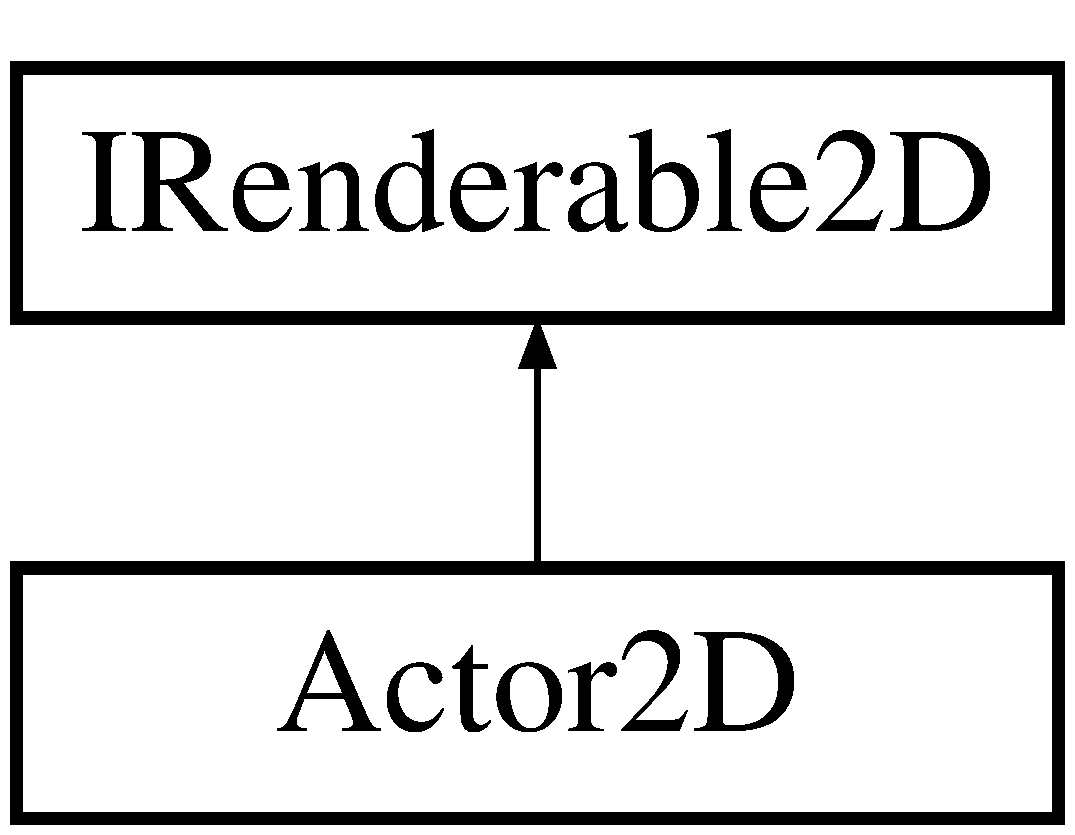
\includegraphics[height=2.000000cm]{classActor2D}
\end{center}
\end{figure}
\subsection*{Additional Inherited Members}


The documentation for this class was generated from the following file\+:\begin{DoxyCompactItemize}
\item 
/home/tsteinholz/\+Development/\+C++/\+Last-\/\+Stand-\/\+Engine/\+Source/\+Graphics/\+Actors/Actor2\+D.\+h\end{DoxyCompactItemize}

\hypertarget{classActor3D}{}\section{Actor3\+D Class Reference}
\label{classActor3D}\index{Actor3\+D@{Actor3\+D}}
Inheritance diagram for Actor3\+D\+:\begin{figure}[H]
\begin{center}
\leavevmode
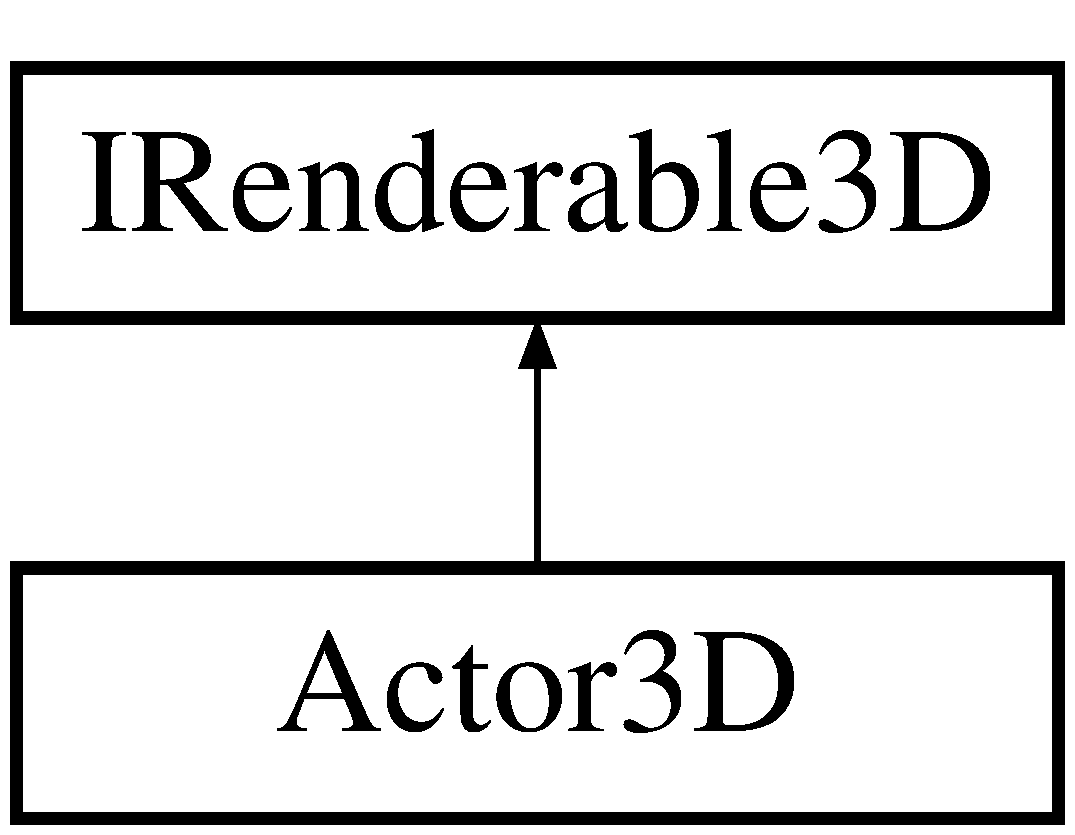
\includegraphics[height=2.000000cm]{classActor3D}
\end{center}
\end{figure}
\subsection*{Additional Inherited Members}


The documentation for this class was generated from the following file\+:\begin{DoxyCompactItemize}
\item 
/home/tsteinholz/\+Development/\+C++/\+Last-\/\+Stand-\/\+Engine/\+Source/\+Graphics/\+Actors/Actor3\+D.\+h\end{DoxyCompactItemize}

\hypertarget{classAudioManager}{}\section{Audio\+Manager Class Reference}
\label{classAudioManager}\index{Audio\+Manager@{Audio\+Manager}}


{\ttfamily \#include $<$Audio\+Manager.\+h$>$}

Inheritance diagram for Audio\+Manager\+:\begin{figure}[H]
\begin{center}
\leavevmode
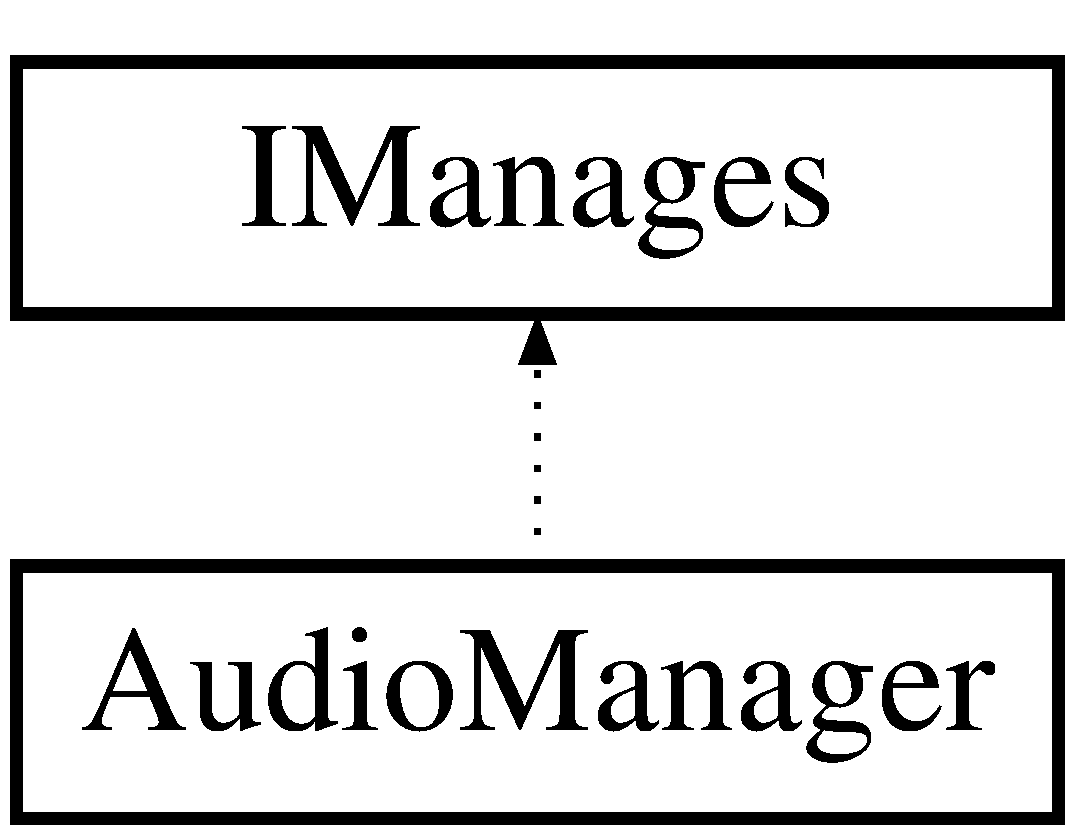
\includegraphics[height=2.000000cm]{classAudioManager}
\end{center}
\end{figure}


\subsection{Detailed Description}
This file is part of the Last Stand Gaming Engine.

The Last Stand Gaming Engine is free software\+: you can redistribute it and/or modify it under the terms of the G\+N\+U General Public License as published by the Free Software Foundation, either version 3 of the License, or (at your option) any later version.

The Last Stand Gaming Engine is distributed in the hope that it will be useful, but W\+I\+T\+H\+O\+U\+T A\+N\+Y W\+A\+R\+R\+A\+N\+T\+Y; without even the implied warranty of M\+E\+R\+C\+H\+A\+N\+T\+A\+B\+I\+L\+I\+T\+Y or F\+I\+T\+N\+E\+S\+S F\+O\+R A P\+A\+R\+T\+I\+C\+U\+L\+A\+R P\+U\+R\+P\+O\+S\+E. See the G\+N\+U General Public License for more details.

You should have received a copy of the G\+N\+U General Public License along with The Last Stand Gaming Engine. If not, see \href{http://www.gnu.org/licenses/}{\tt http\+://www.\+gnu.\+org/licenses/}. 

The documentation for this class was generated from the following file\+:\begin{DoxyCompactItemize}
\item 
/home/tsteinholz/\+Development/\+C++/\+Last-\/\+Stand-\/\+Engine/\+Source/\+Audio/Audio\+Manager.\+h\end{DoxyCompactItemize}

\hypertarget{classFile}{}\section{File Class Reference}
\label{classFile}\index{File@{File}}


The documentation for this class was generated from the following file\+:\begin{DoxyCompactItemize}
\item 
/home/tsteinholz/\+Development/\+C++/\+Last-\/\+Stand-\/\+Engine/\+Source/\+Files/File.\+h\end{DoxyCompactItemize}

\hypertarget{classIManages}{}\section{I\+Manages Class Reference}
\label{classIManages}\index{I\+Manages@{I\+Manages}}


{\ttfamily \#include $<$I\+Manages.\+h$>$}

Inheritance diagram for I\+Manages\+:\begin{figure}[H]
\begin{center}
\leavevmode
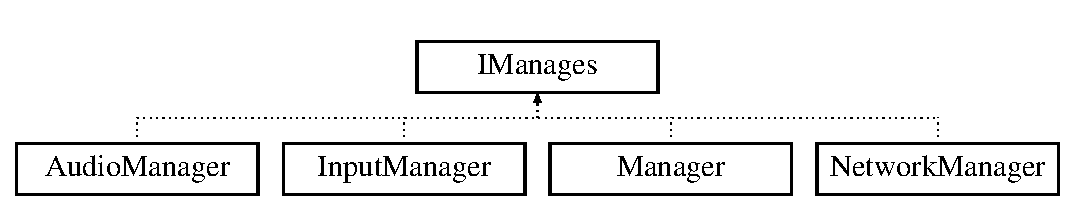
\includegraphics[height=2.000000cm]{classIManages}
\end{center}
\end{figure}


\subsection{Detailed Description}
This is the interface that every manager should implement. It contains all of the most generic and basic functions of all managers which keeps consistency and code efficiency. 

The documentation for this class was generated from the following file\+:\begin{DoxyCompactItemize}
\item 
/home/tsteinholz/\+Development/\+C++/\+Last-\/\+Stand-\/\+Engine/\+Source/\+Core/I\+Manages.\+h\end{DoxyCompactItemize}

\hypertarget{classInputManager}{}\section{Input\+Manager Class Reference}
\label{classInputManager}\index{Input\+Manager@{Input\+Manager}}
Inheritance diagram for Input\+Manager\+:\begin{figure}[H]
\begin{center}
\leavevmode
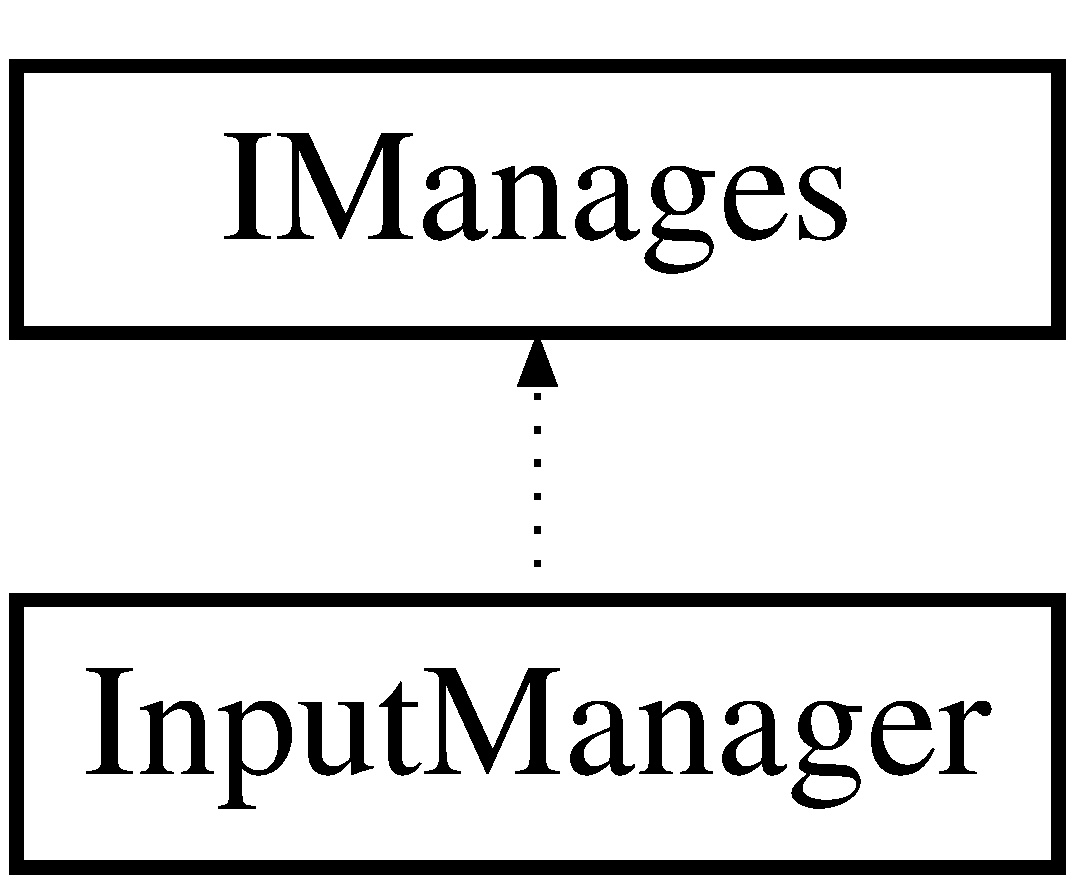
\includegraphics[height=2.000000cm]{classInputManager}
\end{center}
\end{figure}


The documentation for this class was generated from the following file\+:\begin{DoxyCompactItemize}
\item 
/home/tsteinholz/\+Development/\+C++/\+Last-\/\+Stand-\/\+Engine/\+Source/\+Input/Input\+Manager.\+h\end{DoxyCompactItemize}

\hypertarget{classIRenderable2D}{}\section{I\+Renderable2\+D Class Reference}
\label{classIRenderable2D}\index{I\+Renderable2\+D@{I\+Renderable2\+D}}
Inheritance diagram for I\+Renderable2\+D\+:\begin{figure}[H]
\begin{center}
\leavevmode
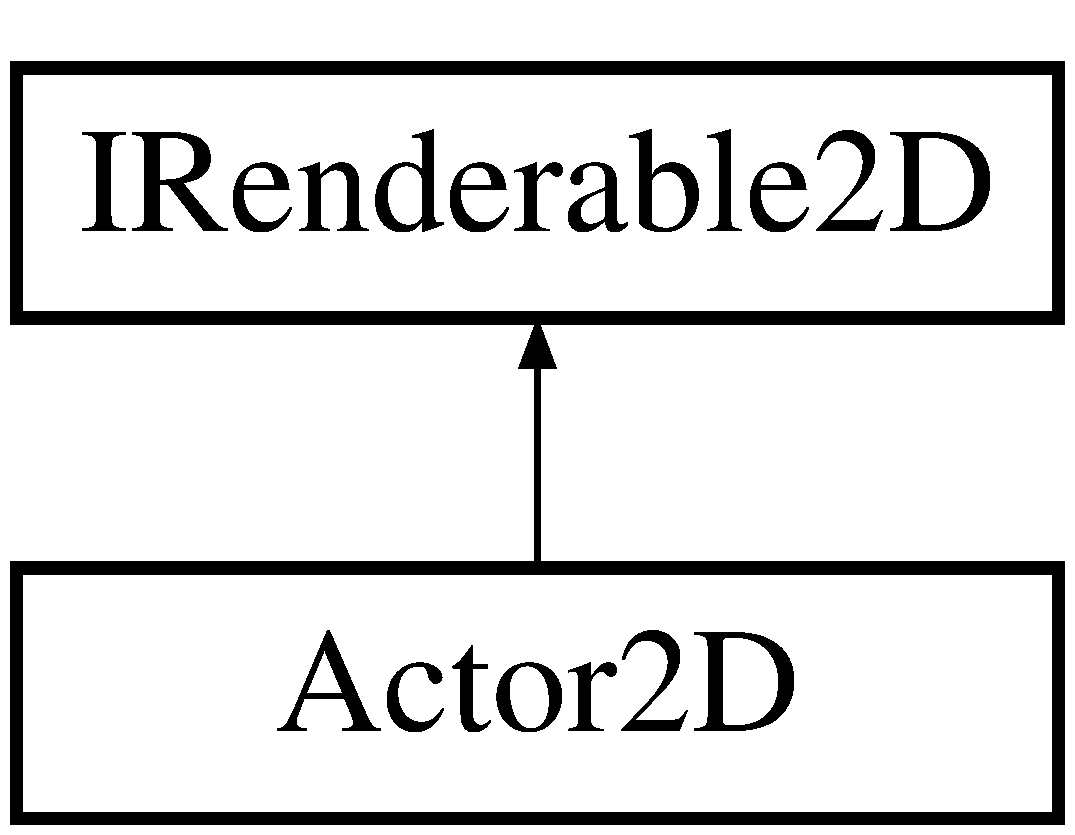
\includegraphics[height=2.000000cm]{classIRenderable2D}
\end{center}
\end{figure}
\subsection*{Public Member Functions}
\begin{DoxyCompactItemize}
\item 
\hypertarget{classIRenderable2D_acc3b3129a444ecadf45ec0ad000aa92c}{}virtual void {\bfseries Update} (float delta)\label{classIRenderable2D_acc3b3129a444ecadf45ec0ad000aa92c}

\item 
\hypertarget{classIRenderable2D_a8a462af175a5e739b96d6833d714772c}{}virtual void {\bfseries Render} ()\label{classIRenderable2D_a8a462af175a5e739b96d6833d714772c}

\item 
\hypertarget{classIRenderable2D_ae4d37c880f417d12b9ded4a486719fa2}{}void {\bfseries Destroy} ()\label{classIRenderable2D_ae4d37c880f417d12b9ded4a486719fa2}

\item 
\hypertarget{classIRenderable2D_afc585cdcf0697bdf6ee691836df40029}{}bool {\bfseries Is\+Destroyed} ()\label{classIRenderable2D_afc585cdcf0697bdf6ee691836df40029}

\item 
\hypertarget{classIRenderable2D_abc4275273450d0200dbba48662b842d6}{}int {\bfseries Get2\+D\+Layer} ()\label{classIRenderable2D_abc4275273450d0200dbba48662b842d6}

\end{DoxyCompactItemize}
\subsection*{Protected Member Functions}
\begin{DoxyCompactItemize}
\item 
\hypertarget{classIRenderable2D_ab28305f75adffc51d7cfae5be4ed0aeb}{}virtual void {\bfseries Pre\+Destroy} ()\label{classIRenderable2D_ab28305f75adffc51d7cfae5be4ed0aeb}

\end{DoxyCompactItemize}
\subsection*{Friends}
\begin{DoxyCompactItemize}
\item 
\hypertarget{classIRenderable2D_ac4da8dd404a2eaf5a0bd84aeb8de1197}{}class {\bfseries Universe}\label{classIRenderable2D_ac4da8dd404a2eaf5a0bd84aeb8de1197}

\end{DoxyCompactItemize}


The documentation for this class was generated from the following file\+:\begin{DoxyCompactItemize}
\item 
/home/tsteinholz/\+Development/\+C++/\+Last-\/\+Stand-\/\+Engine/\+Source/\+Graphics/I\+Renderable2\+D.\+h\end{DoxyCompactItemize}

\hypertarget{classIRenderable3D}{}\section{I\+Renderable3\+D Class Reference}
\label{classIRenderable3D}\index{I\+Renderable3\+D@{I\+Renderable3\+D}}
Inheritance diagram for I\+Renderable3\+D\+:\begin{figure}[H]
\begin{center}
\leavevmode
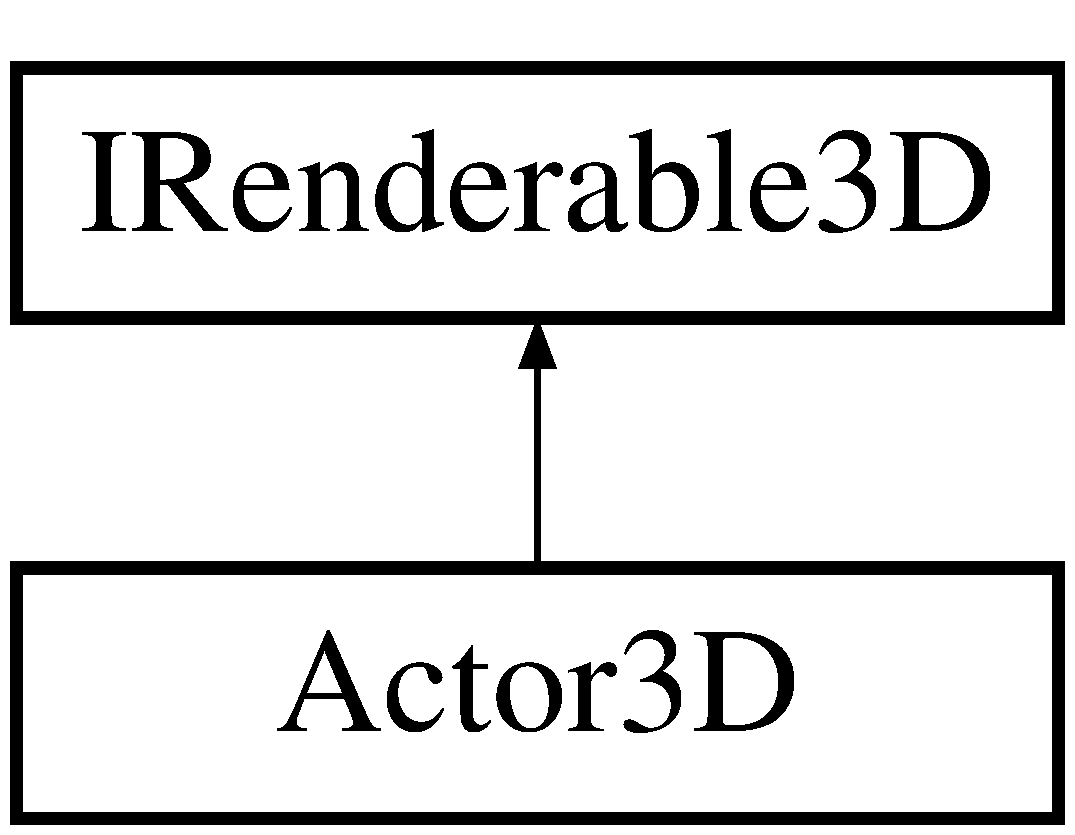
\includegraphics[height=2.000000cm]{classIRenderable3D}
\end{center}
\end{figure}
\subsection*{Protected Member Functions}
\begin{DoxyCompactItemize}
\item 
\hypertarget{classIRenderable3D_acb5030f72e1b2eb8ae3d119fc89d75bb}{}virtual void {\bfseries Pre\+Destroy} ()\label{classIRenderable3D_acb5030f72e1b2eb8ae3d119fc89d75bb}

\end{DoxyCompactItemize}
\subsection*{Friends}
\begin{DoxyCompactItemize}
\item 
\hypertarget{classIRenderable3D_ac4da8dd404a2eaf5a0bd84aeb8de1197}{}class {\bfseries Universe}\label{classIRenderable3D_ac4da8dd404a2eaf5a0bd84aeb8de1197}

\end{DoxyCompactItemize}


The documentation for this class was generated from the following file\+:\begin{DoxyCompactItemize}
\item 
/home/tsteinholz/\+Development/\+C++/\+Last-\/\+Stand-\/\+Engine/\+Source/\+Graphics/I\+Renderable3\+D.\+h\end{DoxyCompactItemize}

\hypertarget{classLog}{}\section{Log Class Reference}
\label{classLog}\index{Log@{Log}}
\subsection*{Public Member Functions}
\begin{DoxyCompactItemize}
\item 
\hypertarget{classLog_a0a319aee4f9b3df2d33b58ebd6f16240}{}{\bfseries Log} (const std\+::string \&f\+Name)\label{classLog_a0a319aee4f9b3df2d33b58ebd6f16240}

\item 
\hypertarget{classLog_ad86b6d7390d3ffcb86e8b5eea46748f0}{}{\footnotesize template$<$class T $>$ }\\\hyperlink{classLog}{Log} \& {\bfseries operator$<$$<$} (const T \&a)\label{classLog_ad86b6d7390d3ffcb86e8b5eea46748f0}

\end{DoxyCompactItemize}


The documentation for this class was generated from the following file\+:\begin{DoxyCompactItemize}
\item 
/home/tsteinholz/\+Development/\+C++/\+Last-\/\+Stand-\/\+Engine/\+Source/\+Utils/Log.\+h\end{DoxyCompactItemize}

\hypertarget{classManager}{}\section{Manager Class Reference}
\label{classManager}\index{Manager@{Manager}}


{\ttfamily \#include $<$Manager.\+h$>$}

Inheritance diagram for Manager\+:\begin{figure}[H]
\begin{center}
\leavevmode
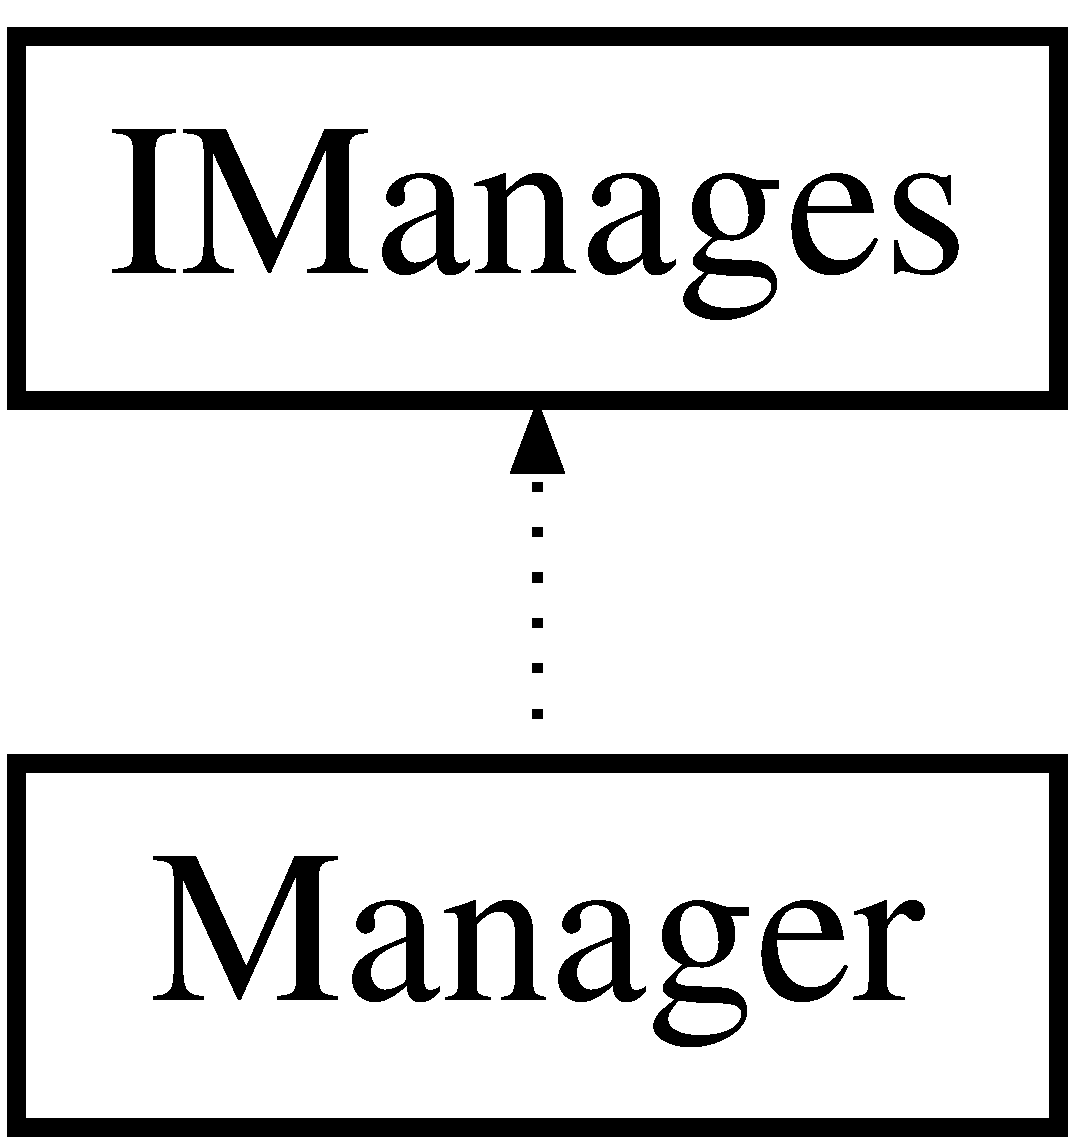
\includegraphics[height=2.000000cm]{classManager}
\end{center}
\end{figure}
\subsection*{Public Member Functions}
\begin{DoxyCompactItemize}
\item 
\hypertarget{classManager_a858943fdd03bfb1c692c56482094e3a0}{}\hyperlink{classManager}{Manager} \& {\bfseries Get\+Instance} ()\label{classManager_a858943fdd03bfb1c692c56482094e3a0}

\end{DoxyCompactItemize}
\subsection*{Static Public Attributes}
\begin{DoxyCompactItemize}
\item 
\hypertarget{classManager_a24e66f6bd92ae6dcb6853d4f9a24c919}{}static \hyperlink{classAudioManager}{Audio\+Manager} $\ast$ {\bfseries Audio}\label{classManager_a24e66f6bd92ae6dcb6853d4f9a24c919}

\item 
\hypertarget{classManager_af9a422e393f203745c8711143e2b28f2}{}static \hyperlink{classInputManager}{Input\+Manager} $\ast$ {\bfseries Inputs}\label{classManager_af9a422e393f203745c8711143e2b28f2}

\item 
\hypertarget{classManager_ad69b402c809daa162b40b0344dbe691e}{}static \hyperlink{classNetworkManager}{Network\+Manager} $\ast$ {\bfseries Network}\label{classManager_ad69b402c809daa162b40b0344dbe691e}

\end{DoxyCompactItemize}


\subsection{Detailed Description}
This is the master of all managers. This class will be active in every game, to keep everything managed as efficiently as possible. This class is designed to have only one instance running all the time, this means that the class has been designed very modular and efficient. 

The documentation for this class was generated from the following file\+:\begin{DoxyCompactItemize}
\item 
/home/tsteinholz/\+Development/\+C++/\+Last-\/\+Stand-\/\+Engine/\+Source/\+Core/Manager.\+h\end{DoxyCompactItemize}

\hypertarget{classMath}{}\section{Math Class Reference}
\label{classMath}\index{Math@{Math}}


{\ttfamily \#include $<$Math.\+h$>$}

\subsection*{Static Public Member Functions}
\begin{DoxyCompactItemize}
\item 
\hypertarget{classMath_a96af82aa95382f06bb03b77ea4d12b97}{}{\footnotesize template$<$typename T $>$ }\\static T {\bfseries Abs} (T val)\label{classMath_a96af82aa95382f06bb03b77ea4d12b97}

\item 
\hypertarget{classMath_a58130e6975b437305c5865512beb907e}{}{\footnotesize template$<$typename T $>$ }\\static T {\bfseries Max} (T value1, T value2)\label{classMath_a58130e6975b437305c5865512beb907e}

\item 
\hypertarget{classMath_ad60f8423ebf30d2344e44fd2e0647b7b}{}{\footnotesize template$<$typename T $>$ }\\static T {\bfseries Min} (T value1, T value2)\label{classMath_ad60f8423ebf30d2344e44fd2e0647b7b}

\item 
\hypertarget{classMath_aec8ac4b0934a6f1c6ad60557d750a70e}{}{\footnotesize template$<$typename T $>$ }\\static T {\bfseries Distance} (T value1, T value2)\label{classMath_aec8ac4b0934a6f1c6ad60557d750a70e}

\item 
\hypertarget{classMath_a54159ad92ccae10fb8e4cb1b7e1ede0d}{}{\footnotesize template$<$typename T $>$ }\\static T {\bfseries Lerp} (T value1, T value2, float amount)\label{classMath_a54159ad92ccae10fb8e4cb1b7e1ede0d}

\item 
\hypertarget{classMath_af09efd8de760e53a9cbefd755848e908}{}{\footnotesize template$<$typename T $>$ }\\static T {\bfseries Smooth\+Step} (T value1, T value2, float amount)\label{classMath_af09efd8de760e53a9cbefd755848e908}

\item 
\hypertarget{classMath_a47a54d98163a26bd779e5d55ada04212}{}static int {\bfseries Clamp} (int value, int min, int max)\label{classMath_a47a54d98163a26bd779e5d55ada04212}

\item 
\hypertarget{classMath_ae95e11ecbc56f98783b705377b9b29d2}{}static float {\bfseries Clamp} (float value, float min, float max)\label{classMath_ae95e11ecbc56f98783b705377b9b29d2}

\item 
\hypertarget{classMath_a7a5fc41dc7f58dff7611bbb494696a2d}{}static double {\bfseries Clamp} (double value, double min, double max)\label{classMath_a7a5fc41dc7f58dff7611bbb494696a2d}

\item 
\hypertarget{classMath_a140507f920c52298914a22d9c666b916}{}static float {\bfseries To\+Degrees} (float radians)\label{classMath_a140507f920c52298914a22d9c666b916}

\item 
\hypertarget{classMath_abd1d206e5441e7ae57ac4dcbcd1c952d}{}static float {\bfseries To\+Radians} (float degrees)\label{classMath_abd1d206e5441e7ae57ac4dcbcd1c952d}

\item 
\hypertarget{classMath_a53f4aaa015bfa0e025f2544fa1808a7f}{}static int {\bfseries Round\+Int} (double x)\label{classMath_a53f4aaa015bfa0e025f2544fa1808a7f}

\item 
\hypertarget{classMath_a0234dd2c80df9d3b33133aa1851e5987}{}static int {\bfseries Random\+Int} (int maximum=1)\label{classMath_a0234dd2c80df9d3b33133aa1851e5987}

\item 
\hypertarget{classMath_a7055d51fea793c221a20acadf028491d}{}static int {\bfseries Random\+Int} (int min, int max)\label{classMath_a7055d51fea793c221a20acadf028491d}

\item 
\hypertarget{classMath_ad884a7d84873d241b284e7191821e393}{}static float {\bfseries Random\+Float} (float maximum=1.\+0f)\label{classMath_ad884a7d84873d241b284e7191821e393}

\item 
\hypertarget{classMath_a578f0941c04d0b8ec7053cf790605b62}{}static float {\bfseries Random\+Float} (float min, float max)\label{classMath_a578f0941c04d0b8ec7053cf790605b62}

\item 
\hypertarget{classMath_a7ed06a614e5fb8fe9c9681e4bf7ffa7c}{}static bool {\bfseries Random\+Bool} ()\label{classMath_a7ed06a614e5fb8fe9c9681e4bf7ffa7c}

\end{DoxyCompactItemize}
\subsection*{Static Public Attributes}
\begin{DoxyCompactItemize}
\item 
\hypertarget{classMath_af648460e9df0272cc721d00b31181e75}{}static const float {\bfseries E} = 2.\+718282f\label{classMath_af648460e9df0272cc721d00b31181e75}

\item 
\hypertarget{classMath_a07e4ce5c7bcec873c3d4671c9aed11a8}{}static const float {\bfseries Log10\+E} = 0.\+4342945f\label{classMath_a07e4ce5c7bcec873c3d4671c9aed11a8}

\item 
\hypertarget{classMath_a0212609a0369ceeb04b9a64b228b76fc}{}static const float {\bfseries Log2\+E} = 1.\+442695f\label{classMath_a0212609a0369ceeb04b9a64b228b76fc}

\item 
\hypertarget{classMath_abc2f17b5e6cb4da17f718364aedafa8e}{}static const float {\bfseries Pi} = 3.\+141593f\label{classMath_abc2f17b5e6cb4da17f718364aedafa8e}

\item 
\hypertarget{classMath_a81d1e8c9e6150ed218f0d01b68dfdbcd}{}static const float {\bfseries Two\+Pi}\label{classMath_a81d1e8c9e6150ed218f0d01b68dfdbcd}

\item 
\hypertarget{classMath_a2835e5027d6e945147b6ad7d532cdd58}{}static const float {\bfseries Max\+Float} = 3.\+402823\+E+38f\label{classMath_a2835e5027d6e945147b6ad7d532cdd58}

\item 
\hypertarget{classMath_aa72ba3b8a773f863f4437cc3c7c973d5}{}static const float {\bfseries Min\+Float} = -\/3.\+402823\+E+38f\label{classMath_aa72ba3b8a773f863f4437cc3c7c973d5}

\item 
\hypertarget{classMath_a7c0c0c1e493031bf06586b726a27be4e}{}static const int {\bfseries Max\+Int} = 2147483648\label{classMath_a7c0c0c1e493031bf06586b726a27be4e}

\item 
\hypertarget{classMath_a89d6f8e36b555b6687f69c12fdb68120}{}static const int {\bfseries Min\+Int} = -\/2147483648\label{classMath_a89d6f8e36b555b6687f69c12fdb68120}

\item 
\hypertarget{classMath_a3ed97c5d5004d8f35fa4eb2a80b9c2a2}{}static const float {\bfseries Epsilon} = 0.\+000001f\label{classMath_a3ed97c5d5004d8f35fa4eb2a80b9c2a2}

\end{DoxyCompactItemize}


\subsection{Detailed Description}
A generic \hyperlink{classMath}{Math} Class to make difficult equations easy with correctness and efficiency. The following class has useful functions and constants you would find in your average graphing calculator. Except a little bit more centered towards video-\/games and the math involved in making them work. 

The documentation for this class was generated from the following files\+:\begin{DoxyCompactItemize}
\item 
/home/tsteinholz/\+Development/\+C++/\+Last-\/\+Stand-\/\+Engine/\+Source/\+Math/Math.\+h\item 
/home/tsteinholz/\+Development/\+C++/\+Last-\/\+Stand-\/\+Engine/\+Source/\+Math/Math.\+cpp\end{DoxyCompactItemize}

\hypertarget{classMatrix}{}\section{Matrix Class Reference}
\label{classMatrix}\index{Matrix@{Matrix}}


The documentation for this class was generated from the following file\+:\begin{DoxyCompactItemize}
\item 
/home/tsteinholz/\+Development/\+C++/\+Last-\/\+Stand-\/\+Engine/\+Source/\+Math/Matrix.\+h\end{DoxyCompactItemize}

\hypertarget{classNetworkManager}{}\section{Network\+Manager Class Reference}
\label{classNetworkManager}\index{Network\+Manager@{Network\+Manager}}


{\ttfamily \#include $<$Network\+Manager.\+h$>$}

Inheritance diagram for Network\+Manager\+:\begin{figure}[H]
\begin{center}
\leavevmode
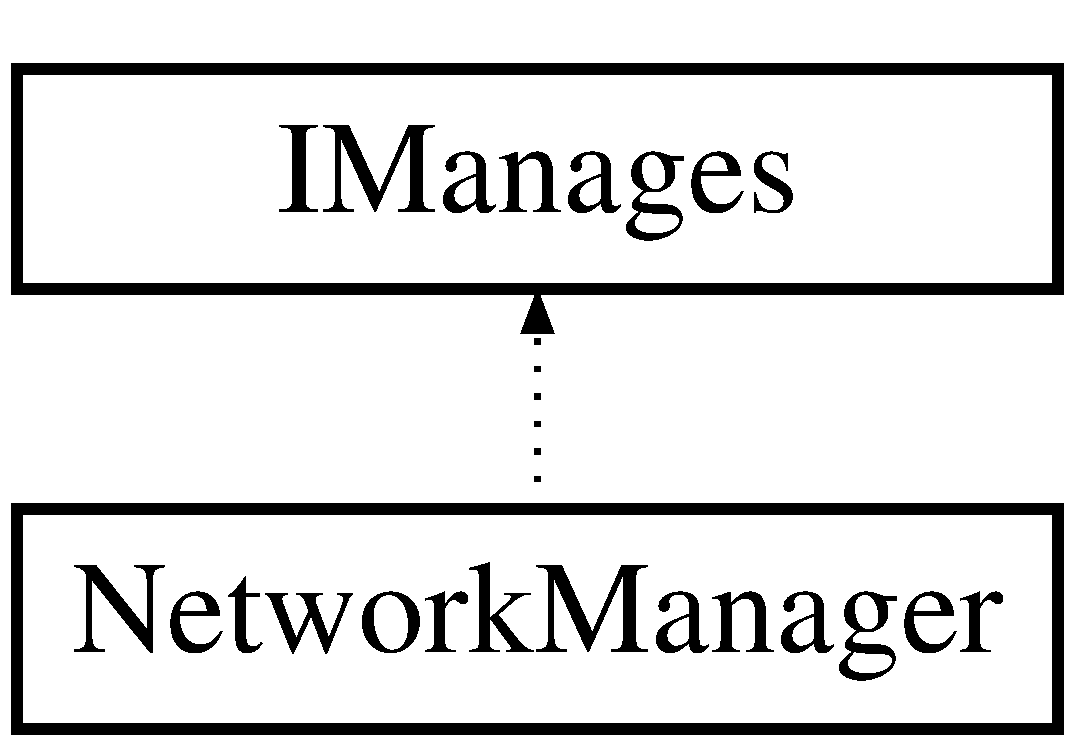
\includegraphics[height=2.000000cm]{classNetworkManager}
\end{center}
\end{figure}


\subsection{Detailed Description}
This Class takes care of and manages all network connections, form p2p \& server multi-\/player. To http streaming form web servers. Anything to do with networking will be accessible from this class and will manage it in the most efficient and speedy way possible. 

The documentation for this class was generated from the following file\+:\begin{DoxyCompactItemize}
\item 
/home/tsteinholz/\+Development/\+C++/\+Last-\/\+Stand-\/\+Engine/\+Source/\+Networking/Network\+Manager.\+h\end{DoxyCompactItemize}

\hypertarget{classPlane}{}\section{Plane Class Reference}
\label{classPlane}\index{Plane@{Plane}}


The documentation for this class was generated from the following file\+:\begin{DoxyCompactItemize}
\item 
/home/tsteinholz/\+Development/\+C++/\+Last-\/\+Stand-\/\+Engine/\+Source/\+Math/Plane.\+h\end{DoxyCompactItemize}

\hypertarget{classQuaternion}{}\section{Quaternion Class Reference}
\label{classQuaternion}\index{Quaternion@{Quaternion}}


The documentation for this class was generated from the following file\+:\begin{DoxyCompactItemize}
\item 
/home/tsteinholz/\+Development/\+C++/\+Last-\/\+Stand-\/\+Engine/\+Source/\+Math/Quaternion.\+h\end{DoxyCompactItemize}

\hypertarget{classUniverse}{}\section{Universe Class Reference}
\label{classUniverse}\index{Universe@{Universe}}


{\ttfamily \#include $<$Universe.\+h$>$}

\subsection*{Public Types}
\begin{DoxyCompactItemize}
\item 
enum \hyperlink{classUniverse_a9a3907e0a49d7e91098163238ef50505}{Engine\+State} \{ \hyperlink{classUniverse_a9a3907e0a49d7e91098163238ef50505a2ccf20ffb4fe4beb8d5f01e138ad4e72}{S\+T\+A\+R\+T\+I\+N\+G} = 0, 
\hyperlink{classUniverse_a9a3907e0a49d7e91098163238ef50505ae8454679e33e08f1a27b6cf469155c3a}{I\+N\+I\+T\+I\+A\+L\+I\+Z\+I\+N\+G} = 1, 
\hyperlink{classUniverse_a9a3907e0a49d7e91098163238ef50505a291f8ef62e9f213687e37c52a41b49b5}{R\+U\+N\+N\+I\+N\+G} = 2, 
\hyperlink{classUniverse_a9a3907e0a49d7e91098163238ef50505a09af4dbe08a6b4c30e16ca60dc814f03}{S\+T\+O\+P\+I\+N\+G} = 3
 \}
\end{DoxyCompactItemize}
\subsection*{Public Member Functions}
\begin{DoxyCompactItemize}
\item 
bool \hyperlink{classUniverse_a3860ac71f57025031201a3ae5c110f1d}{Initialize} (unsigned int window\+Width=800, unsigned int window\+Height=600, const std\+::string \&window\+Title=\char`\"{}Last Stand Engine\char`\"{}, bool x\+\_\+\+Anti\+Aliasing=true, bool full\+Screen=false, bool resizable=true)
\item 
\hypertarget{classUniverse_a8789e78de0e3b22175a853afc38596e6}{}void {\bfseries Start} ()\label{classUniverse_a8789e78de0e3b22175a853afc38596e6}

\item 
\hypertarget{classUniverse_ac0d229ce70112bbbf760f5ca0864aa9d}{}void {\bfseries Pause} ()\label{classUniverse_ac0d229ce70112bbbf760f5ca0864aa9d}

\item 
\hypertarget{classUniverse_ae38c939451fc5eea5b33cd5ff4c4ce8e}{}void {\bfseries Stop} ()\label{classUniverse_ae38c939451fc5eea5b33cd5ff4c4ce8e}

\end{DoxyCompactItemize}
\subsection*{Static Public Member Functions}
\begin{DoxyCompactItemize}
\item 
static \hyperlink{classUniverse}{Universe} \& \hyperlink{classUniverse_a7a9e1c0df0fea192e0ead1fbd3e35d1e}{Get\+Instance} ()
\end{DoxyCompactItemize}
\subsection*{Public Attributes}
\begin{DoxyCompactItemize}
\item 
\hyperlink{classUniverse_a9a3907e0a49d7e91098163238ef50505}{Engine\+State} \hyperlink{classUniverse_a8da2dd7a1c2bb9b7e0447e06ef61df5c}{The\+Engine\+State}
\end{DoxyCompactItemize}


\subsection{Detailed Description}
This is the mother class of the game. This Class represnts the entire game, thus its name \char`\"{}\+The Universe\char`\"{}. Everything that goes on in the game will go on in the universe (this class). This makes levels and code eaier to manage. 

\subsection{Member Enumeration Documentation}
\hypertarget{classUniverse_a9a3907e0a49d7e91098163238ef50505}{}\index{Universe@{Universe}!Engine\+State@{Engine\+State}}
\index{Engine\+State@{Engine\+State}!Universe@{Universe}}
\subsubsection[{Engine\+State}]{\setlength{\rightskip}{0pt plus 5cm}enum {\bf Universe\+::\+Engine\+State}}\label{classUniverse_a9a3907e0a49d7e91098163238ef50505}
The diffrent modes and states that the Game Engine could possibly be in. \begin{Desc}
\item[Enumerator]\par
\begin{description}
\index{S\+T\+A\+R\+T\+I\+N\+G@{S\+T\+A\+R\+T\+I\+N\+G}!Universe@{Universe}}\index{Universe@{Universe}!S\+T\+A\+R\+T\+I\+N\+G@{S\+T\+A\+R\+T\+I\+N\+G}}\item[{\em 
\hypertarget{classUniverse_a9a3907e0a49d7e91098163238ef50505a2ccf20ffb4fe4beb8d5f01e138ad4e72}{}S\+T\+A\+R\+T\+I\+N\+G\label{classUniverse_a9a3907e0a49d7e91098163238ef50505a2ccf20ffb4fe4beb8d5f01e138ad4e72}
}]This is the very first state when the engine gets executed, used mainly for set-\/up. The atcual window creation is done in the Initialization step. \index{I\+N\+I\+T\+I\+A\+L\+I\+Z\+I\+N\+G@{I\+N\+I\+T\+I\+A\+L\+I\+Z\+I\+N\+G}!Universe@{Universe}}\index{Universe@{Universe}!I\+N\+I\+T\+I\+A\+L\+I\+Z\+I\+N\+G@{I\+N\+I\+T\+I\+A\+L\+I\+Z\+I\+N\+G}}\item[{\em 
\hypertarget{classUniverse_a9a3907e0a49d7e91098163238ef50505ae8454679e33e08f1a27b6cf469155c3a}{}I\+N\+I\+T\+I\+A\+L\+I\+Z\+I\+N\+G\label{classUniverse_a9a3907e0a49d7e91098163238ef50505ae8454679e33e08f1a27b6cf469155c3a}
}]At this state the engine is loading the window, all the calls in this state are low-\/level Open\+G\+L calls to get everything running with the proper settings and prefrences configured. \index{R\+U\+N\+N\+I\+N\+G@{R\+U\+N\+N\+I\+N\+G}!Universe@{Universe}}\index{Universe@{Universe}!R\+U\+N\+N\+I\+N\+G@{R\+U\+N\+N\+I\+N\+G}}\item[{\em 
\hypertarget{classUniverse_a9a3907e0a49d7e91098163238ef50505a291f8ef62e9f213687e37c52a41b49b5}{}R\+U\+N\+N\+I\+N\+G\label{classUniverse_a9a3907e0a49d7e91098163238ef50505a291f8ef62e9f213687e37c52a41b49b5}
}]This is the Engine State that it should be in most of the time. In this state the programmer has the most amount of controll over the game and what it doing. \index{S\+T\+O\+P\+I\+N\+G@{S\+T\+O\+P\+I\+N\+G}!Universe@{Universe}}\index{Universe@{Universe}!S\+T\+O\+P\+I\+N\+G@{S\+T\+O\+P\+I\+N\+G}}\item[{\em 
\hypertarget{classUniverse_a9a3907e0a49d7e91098163238ef50505a09af4dbe08a6b4c30e16ca60dc814f03}{}S\+T\+O\+P\+I\+N\+G\label{classUniverse_a9a3907e0a49d7e91098163238ef50505a09af4dbe08a6b4c30e16ca60dc814f03}
}]At this state the engine has been told to close one way or another. This is when everything should get to a stopping point because it will soon be removed from memory. \end{description}
\end{Desc}


\subsection{Member Function Documentation}
\hypertarget{classUniverse_a7a9e1c0df0fea192e0ead1fbd3e35d1e}{}\index{Universe@{Universe}!Get\+Instance@{Get\+Instance}}
\index{Get\+Instance@{Get\+Instance}!Universe@{Universe}}
\subsubsection[{Get\+Instance}]{\setlength{\rightskip}{0pt plus 5cm}{\bf Universe} \& Universe\+::\+Get\+Instance (
\begin{DoxyParamCaption}
{}
\end{DoxyParamCaption}
)\hspace{0.3cm}{\ttfamily [static]}}\label{classUniverse_a7a9e1c0df0fea192e0ead1fbd3e35d1e}
This is the method used to get / create the \hyperlink{classUniverse}{Universe}, since there can only be one \hyperlink{classUniverse}{Universe} at a time due to thie Singleton Pattern. This is the only way to get or create a \hyperlink{classUniverse}{Universe}.

\begin{DoxyReturn}{Returns}
The \hyperlink{classUniverse}{Universe} 
\end{DoxyReturn}
\hypertarget{classUniverse_a3860ac71f57025031201a3ae5c110f1d}{}\index{Universe@{Universe}!Initialize@{Initialize}}
\index{Initialize@{Initialize}!Universe@{Universe}}
\subsubsection[{Initialize}]{\setlength{\rightskip}{0pt plus 5cm}bool Universe\+::\+Initialize (
\begin{DoxyParamCaption}
\item[{unsigned int}]{window\+Width = {\ttfamily 800}, }
\item[{unsigned int}]{window\+Height = {\ttfamily 600}, }
\item[{const std\+::string \&}]{window\+Title = {\ttfamily \char`\"{}Last~Stand~Engine\char`\"{}}, }
\item[{bool}]{x\+\_\+\+Anti\+Aliasing = {\ttfamily true}, }
\item[{bool}]{full\+Screen = {\ttfamily false}, }
\item[{bool}]{resizable = {\ttfamily true}}
\end{DoxyParamCaption}
)}\label{classUniverse_a3860ac71f57025031201a3ae5c110f1d}
This is the method used to set up the \hyperlink{classUniverse}{Universe}. Since The Singleton Pattern is being used here, this is the closest thing to a constructor. The settings can only inserted in this function one time, to change any settings a diffrent method must be used.

\begin{DoxyReturn}{Returns}
true if successful. 
\end{DoxyReturn}


\subsection{Member Data Documentation}
\hypertarget{classUniverse_a8da2dd7a1c2bb9b7e0447e06ef61df5c}{}\index{Universe@{Universe}!The\+Engine\+State@{The\+Engine\+State}}
\index{The\+Engine\+State@{The\+Engine\+State}!Universe@{Universe}}
\subsubsection[{The\+Engine\+State}]{\setlength{\rightskip}{0pt plus 5cm}{\bf Engine\+State} Universe\+::\+The\+Engine\+State}\label{classUniverse_a8da2dd7a1c2bb9b7e0447e06ef61df5c}
This is the current Engine State of the Engine in real time and will only be modified by the \hyperlink{classUniverse}{Universe} itself. 

The documentation for this class was generated from the following files\+:\begin{DoxyCompactItemize}
\item 
/home/tsteinholz/\+Development/\+C++/\+Last-\/\+Stand-\/\+Engine/\+Source/\+Core/Universe.\+h\item 
/home/tsteinholz/\+Development/\+C++/\+Last-\/\+Stand-\/\+Engine/\+Source/\+Core/Universe.\+cpp\end{DoxyCompactItemize}

\hypertarget{classLastStandEngine_1_1Utils_1_1Utils}{}\section{Last\+Stand\+Engine\+:\+:Utils\+:\+:Utils Class Reference}
\label{classLastStandEngine_1_1Utils_1_1Utils}\index{Last\+Stand\+Engine\+::\+Utils\+::\+Utils@{Last\+Stand\+Engine\+::\+Utils\+::\+Utils}}


The documentation for this class was generated from the following file\+:\begin{DoxyCompactItemize}
\item 
/home/tsteinholz/\+Development/\+C++/\+Last-\/\+Stand-\/\+Engine/\+Source/\+Utils/Utils.\+h\end{DoxyCompactItemize}

\hypertarget{structVector2}{}\section{Vector2 Struct Reference}
\label{structVector2}\index{Vector2@{Vector2}}


{\ttfamily \#include $<$Vector2.\+h$>$}

\subsection*{Public Types}
\begin{DoxyCompactItemize}
\item 
\hypertarget{structVector2_adab03c8453d61490400f44dc95b1ec3f}{}typedef std\+::vector$<$ \hyperlink{structVector2}{Vector2} $>$ {\bfseries Vector2\+List}\label{structVector2_adab03c8453d61490400f44dc95b1ec3f}

\end{DoxyCompactItemize}
\subsection*{Public Member Functions}
\begin{DoxyCompactItemize}
\item 
\hyperlink{structVector2_a22104d1809be26a419ef1f959e3761bf}{Vector2} ()
\item 
\hyperlink{structVector2_a061ab58a0e216c759d64e3746d712b12}{Vector2} (float x, float y)
\item 
\hyperlink{structVector2_afea54870cbfd859a8cefddde63c1eade}{Vector2} (float val)
\item 
\hyperlink{structVector2_a11a9a7497a068a1be452c7308a742baa}{Vector2} (const \hyperlink{structVector2}{Vector2} \&copy)
\item 
float \hyperlink{structVector2_ae7b80a14336e86c30a11218cd27a4abf}{Length} ()
\item 
float \hyperlink{structVector2_abb8185e17df25af915a6490028a47220}{Length\+Squared} ()
\item 
void \hyperlink{structVector2_a3b597b3bfeb114dd9e157b86330e087d}{Normalize} ()
\item 
\hypertarget{structVector2_a41cc3205bc01ec255df48b93654617c8}{}bool {\bfseries operator==} (const \hyperlink{structVector2}{Vector2} \&v) const \label{structVector2_a41cc3205bc01ec255df48b93654617c8}

\item 
\hypertarget{structVector2_a0ad61ef61851d0efb7cddd5ba9353ef3}{}bool {\bfseries operator!=} (const \hyperlink{structVector2}{Vector2} \&v) const \label{structVector2_a0ad61ef61851d0efb7cddd5ba9353ef3}

\item 
\hypertarget{structVector2_a5f5eb2d81dd299366ca228963ae76fa0}{}\hyperlink{structVector2}{Vector2} {\bfseries operator-\/} () const \label{structVector2_a5f5eb2d81dd299366ca228963ae76fa0}

\item 
\hypertarget{structVector2_a39dfeea6e55ef1df7b819cf35efd4a79}{}\hyperlink{structVector2}{Vector2} {\bfseries operator-\/} (const \hyperlink{structVector2}{Vector2} \&v) const \label{structVector2_a39dfeea6e55ef1df7b819cf35efd4a79}

\item 
\hypertarget{structVector2_a93473ed56b2cedcafe3690572eeeec33}{}\hyperlink{structVector2}{Vector2} {\bfseries operator+} (const \hyperlink{structVector2}{Vector2} \&v) const \label{structVector2_a93473ed56b2cedcafe3690572eeeec33}

\item 
\hypertarget{structVector2_a7b24a71970464e53d2aa969dfc588090}{}\hyperlink{structVector2}{Vector2} {\bfseries operator/} (float f) const \label{structVector2_a7b24a71970464e53d2aa969dfc588090}

\item 
\hypertarget{structVector2_ae62c0a280cd3024ddb3fcc84b421ce26}{}\hyperlink{structVector2}{Vector2} {\bfseries operator$\ast$} (float f) const \label{structVector2_ae62c0a280cd3024ddb3fcc84b421ce26}

\item 
\hypertarget{structVector2_a2315357e857ba16eeff4455e911d588c}{}\hyperlink{structVector2}{Vector2} \& {\bfseries operator+=} (const \hyperlink{structVector2}{Vector2} \&v)\label{structVector2_a2315357e857ba16eeff4455e911d588c}

\item 
\hypertarget{structVector2_acef1586ad34e658b975c21978a183931}{}\hyperlink{structVector2}{Vector2} \& {\bfseries operator-\/=} (const \hyperlink{structVector2}{Vector2} \&v)\label{structVector2_acef1586ad34e658b975c21978a183931}

\item 
\hypertarget{structVector2_a1a3a24db025c13e87a22678e5dcac58c}{}\hyperlink{structVector2}{Vector2} \& {\bfseries operator$\ast$=} (float f)\label{structVector2_a1a3a24db025c13e87a22678e5dcac58c}

\item 
\hypertarget{structVector2_aac0772c6ffb590990bc73249e1f11e6b}{}\hyperlink{structVector2}{Vector2} \& {\bfseries operator/=} (float f)\label{structVector2_aac0772c6ffb590990bc73249e1f11e6b}

\end{DoxyCompactItemize}
\subsection*{Static Public Member Functions}
\begin{DoxyCompactItemize}
\item 
static float \hyperlink{structVector2_a39d6d5a11de4aae7a83e9427199ef6c2}{Distance} (const \hyperlink{structVector2}{Vector2} \&vector2a, const \hyperlink{structVector2}{Vector2} \&vector2b)
\item 
static float \hyperlink{structVector2_a6d444c3b9e9c910baef36631a29b74a1}{Distance\+Squared} (const \hyperlink{structVector2}{Vector2} \&vector2a, const \hyperlink{structVector2}{Vector2} \&vector2b)
\item 
static float \hyperlink{structVector2_a7e00cb409fcc5b7a2b6413f60560d7b6}{Dot} (const \hyperlink{structVector2}{Vector2} \&vector2a, const \hyperlink{structVector2}{Vector2} \&vector2b)
\item 
static float \hyperlink{structVector2_a40d05adae410e04f5f1309880140284f}{Cross} (const \hyperlink{structVector2}{Vector2} \&vector2a, \hyperlink{structVector2}{Vector2} \&vector2b)
\item 
static \hyperlink{structVector2}{Vector2} \hyperlink{structVector2_aa1cae4abb133f61b3378392a39b43bec}{Normalize} (const \hyperlink{structVector2}{Vector2} \&vector2)
\item 
static \hyperlink{structVector2}{Vector2} \hyperlink{structVector2_afb6a78234fd9053d9e26484615c1ddf5}{Reflect} (const \hyperlink{structVector2}{Vector2} \&a, const \hyperlink{structVector2}{Vector2} \&b)
\item 
static \hyperlink{structVector2}{Vector2} \hyperlink{structVector2_a22f5fa049e36cbb6da68c2b8cc7db5cd}{Min} (const \hyperlink{structVector2}{Vector2} \&vector2a, const \hyperlink{structVector2}{Vector2} vector2b)
\item 
static \hyperlink{structVector2}{Vector2} \hyperlink{structVector2_abdb5a914f07c4aa760832909a2359668}{Max} (const \hyperlink{structVector2}{Vector2} \&vector2a, const \hyperlink{structVector2}{Vector2} vector2b)
\item 
static \hyperlink{structVector2}{Vector2} \hyperlink{structVector2_a251c5b42d6c0cc70001ecd4235d6f466}{Clamp} (const \hyperlink{structVector2}{Vector2} \&value, const \hyperlink{structVector2}{Vector2} \&max, const \hyperlink{structVector2}{Vector2} \&min)
\item 
static \hyperlink{structVector2}{Vector2} \hyperlink{structVector2_acaf1ed1324308802b3a5f7b96c39d33c}{Lerp} (const \hyperlink{structVector2}{Vector2} \&vector2a, const \hyperlink{structVector2}{Vector2} \&vector2b, float amount)
\end{DoxyCompactItemize}
\subsection*{Public Attributes}
\begin{DoxyCompactItemize}
\item 
float \hyperlink{structVector2_ae01506fa3d0fb79821bee7445a0c7baf}{X}
\item 
float \hyperlink{structVector2_ab79dce0b924a27a639e0a3cb82b20cec}{Y}
\end{DoxyCompactItemize}
\subsection*{Static Public Attributes}
\begin{DoxyCompactItemize}
\item 
static \hyperlink{structVector2}{Vector2} \hyperlink{structVector2_a3eb421c40e7bd2653c01a84fb7e55240}{Zero}
\item 
static \hyperlink{structVector2}{Vector2} \hyperlink{structVector2_a1808fb56c85c5ef0320a0cec16348861}{One}
\item 
static \hyperlink{structVector2}{Vector2} \hyperlink{structVector2_a4327b6f08dfb7c40163797f5f20d93ba}{Unit\+X}
\item 
static \hyperlink{structVector2}{Vector2} \hyperlink{structVector2_a89e4cdd468e6e87b6dd512c04b1a6431}{Unit\+Y}
\end{DoxyCompactItemize}


\subsection{Detailed Description}
A Coordinate Point on the screen that has two instance Variables (X \& Y). 

\subsection{Constructor \& Destructor Documentation}
\hypertarget{structVector2_a22104d1809be26a419ef1f959e3761bf}{}\index{Vector2@{Vector2}!Vector2@{Vector2}}
\index{Vector2@{Vector2}!Vector2@{Vector2}}
\subsubsection[{Vector2}]{\setlength{\rightskip}{0pt plus 5cm}Vector2\+::\+Vector2 (
\begin{DoxyParamCaption}
{}
\end{DoxyParamCaption}
)}\label{structVector2_a22104d1809be26a419ef1f959e3761bf}
Basic Constructor for a \hyperlink{structVector2}{Vector2} object, sets values to 0,0. \hypertarget{structVector2_a061ab58a0e216c759d64e3746d712b12}{}\index{Vector2@{Vector2}!Vector2@{Vector2}}
\index{Vector2@{Vector2}!Vector2@{Vector2}}
\subsubsection[{Vector2}]{\setlength{\rightskip}{0pt plus 5cm}Vector2\+::\+Vector2 (
\begin{DoxyParamCaption}
\item[{float}]{x, }
\item[{float}]{y}
\end{DoxyParamCaption}
)}\label{structVector2_a061ab58a0e216c759d64e3746d712b12}
Complete Constructor for a \hyperlink{structVector2}{Vector2}


\begin{DoxyParams}{Parameters}
{\em x} & \+: X value of the \hyperlink{structVector2}{Vector2}. \\
\hline
{\em y} & \+: Y value of the \hyperlink{structVector2}{Vector2}. \\
\hline
\end{DoxyParams}
\hypertarget{structVector2_afea54870cbfd859a8cefddde63c1eade}{}\index{Vector2@{Vector2}!Vector2@{Vector2}}
\index{Vector2@{Vector2}!Vector2@{Vector2}}
\subsubsection[{Vector2}]{\setlength{\rightskip}{0pt plus 5cm}Vector2\+::\+Vector2 (
\begin{DoxyParamCaption}
\item[{float}]{val}
\end{DoxyParamCaption}
)}\label{structVector2_afea54870cbfd859a8cefddde63c1eade}
Sets the x and y values to the same value.


\begin{DoxyParams}{Parameters}
{\em val} & \+: value going into both x and y. \\
\hline
\end{DoxyParams}
\hypertarget{structVector2_a11a9a7497a068a1be452c7308a742baa}{}\index{Vector2@{Vector2}!Vector2@{Vector2}}
\index{Vector2@{Vector2}!Vector2@{Vector2}}
\subsubsection[{Vector2}]{\setlength{\rightskip}{0pt plus 5cm}Vector2\+::\+Vector2 (
\begin{DoxyParamCaption}
\item[{const {\bf Vector2} \&}]{copy}
\end{DoxyParamCaption}
)}\label{structVector2_a11a9a7497a068a1be452c7308a742baa}
Copies a \hyperlink{structVector2}{Vector2}.


\begin{DoxyParams}{Parameters}
{\em copy} & \+: an exciting \hyperlink{structVector2}{Vector2} with desired values. \\
\hline
\end{DoxyParams}


\subsection{Member Function Documentation}
\hypertarget{structVector2_a251c5b42d6c0cc70001ecd4235d6f466}{}\index{Vector2@{Vector2}!Clamp@{Clamp}}
\index{Clamp@{Clamp}!Vector2@{Vector2}}
\subsubsection[{Clamp}]{\setlength{\rightskip}{0pt plus 5cm}{\bf Vector2} Vector2\+::\+Clamp (
\begin{DoxyParamCaption}
\item[{const {\bf Vector2} \&}]{value, }
\item[{const {\bf Vector2} \&}]{max, }
\item[{const {\bf Vector2} \&}]{min}
\end{DoxyParamCaption}
)\hspace{0.3cm}{\ttfamily [static]}}\label{structVector2_a251c5b42d6c0cc70001ecd4235d6f466}

\begin{DoxyParams}{Parameters}
{\em } & \\
\hline
\end{DoxyParams}
\hypertarget{structVector2_a40d05adae410e04f5f1309880140284f}{}\index{Vector2@{Vector2}!Cross@{Cross}}
\index{Cross@{Cross}!Vector2@{Vector2}}
\subsubsection[{Cross}]{\setlength{\rightskip}{0pt plus 5cm}float Vector2\+::\+Cross (
\begin{DoxyParamCaption}
\item[{const {\bf Vector2} \&}]{vector2a, }
\item[{{\bf Vector2} \&}]{vector2b}
\end{DoxyParamCaption}
)\hspace{0.3cm}{\ttfamily [static]}}\label{structVector2_a40d05adae410e04f5f1309880140284f}

\begin{DoxyParams}{Parameters}
{\em } & \\
\hline
\end{DoxyParams}
\hypertarget{structVector2_a39d6d5a11de4aae7a83e9427199ef6c2}{}\index{Vector2@{Vector2}!Distance@{Distance}}
\index{Distance@{Distance}!Vector2@{Vector2}}
\subsubsection[{Distance}]{\setlength{\rightskip}{0pt plus 5cm}float Vector2\+::\+Distance (
\begin{DoxyParamCaption}
\item[{const {\bf Vector2} \&}]{vector2a, }
\item[{const {\bf Vector2} \&}]{vector2b}
\end{DoxyParamCaption}
)\hspace{0.3cm}{\ttfamily [static]}}\label{structVector2_a39d6d5a11de4aae7a83e9427199ef6c2}

\begin{DoxyParams}{Parameters}
{\em } & \\
\hline
\end{DoxyParams}
\hypertarget{structVector2_a6d444c3b9e9c910baef36631a29b74a1}{}\index{Vector2@{Vector2}!Distance\+Squared@{Distance\+Squared}}
\index{Distance\+Squared@{Distance\+Squared}!Vector2@{Vector2}}
\subsubsection[{Distance\+Squared}]{\setlength{\rightskip}{0pt plus 5cm}float Vector2\+::\+Distance\+Squared (
\begin{DoxyParamCaption}
\item[{const {\bf Vector2} \&}]{vector2a, }
\item[{const {\bf Vector2} \&}]{vector2b}
\end{DoxyParamCaption}
)\hspace{0.3cm}{\ttfamily [static]}}\label{structVector2_a6d444c3b9e9c910baef36631a29b74a1}

\begin{DoxyParams}{Parameters}
{\em } & \\
\hline
\end{DoxyParams}
\hypertarget{structVector2_a7e00cb409fcc5b7a2b6413f60560d7b6}{}\index{Vector2@{Vector2}!Dot@{Dot}}
\index{Dot@{Dot}!Vector2@{Vector2}}
\subsubsection[{Dot}]{\setlength{\rightskip}{0pt plus 5cm}float Vector2\+::\+Dot (
\begin{DoxyParamCaption}
\item[{const {\bf Vector2} \&}]{vector2a, }
\item[{const {\bf Vector2} \&}]{vector2b}
\end{DoxyParamCaption}
)\hspace{0.3cm}{\ttfamily [static]}}\label{structVector2_a7e00cb409fcc5b7a2b6413f60560d7b6}

\begin{DoxyParams}{Parameters}
{\em } & \\
\hline
\end{DoxyParams}
\hypertarget{structVector2_ae7b80a14336e86c30a11218cd27a4abf}{}\index{Vector2@{Vector2}!Length@{Length}}
\index{Length@{Length}!Vector2@{Vector2}}
\subsubsection[{Length}]{\setlength{\rightskip}{0pt plus 5cm}float Vector2\+::\+Length (
\begin{DoxyParamCaption}
{}
\end{DoxyParamCaption}
)}\label{structVector2_ae7b80a14336e86c30a11218cd27a4abf}
\begin{DoxyReturn}{Returns}
\+: 
\end{DoxyReturn}
\hypertarget{structVector2_abb8185e17df25af915a6490028a47220}{}\index{Vector2@{Vector2}!Length\+Squared@{Length\+Squared}}
\index{Length\+Squared@{Length\+Squared}!Vector2@{Vector2}}
\subsubsection[{Length\+Squared}]{\setlength{\rightskip}{0pt plus 5cm}float Vector2\+::\+Length\+Squared (
\begin{DoxyParamCaption}
{}
\end{DoxyParamCaption}
)}\label{structVector2_abb8185e17df25af915a6490028a47220}
\begin{DoxyReturn}{Returns}

\end{DoxyReturn}
\hypertarget{structVector2_acaf1ed1324308802b3a5f7b96c39d33c}{}\index{Vector2@{Vector2}!Lerp@{Lerp}}
\index{Lerp@{Lerp}!Vector2@{Vector2}}
\subsubsection[{Lerp}]{\setlength{\rightskip}{0pt plus 5cm}{\bf Vector2} Vector2\+::\+Lerp (
\begin{DoxyParamCaption}
\item[{const {\bf Vector2} \&}]{vector2a, }
\item[{const {\bf Vector2} \&}]{vector2b, }
\item[{float}]{amount}
\end{DoxyParamCaption}
)\hspace{0.3cm}{\ttfamily [static]}}\label{structVector2_acaf1ed1324308802b3a5f7b96c39d33c}

\begin{DoxyParams}{Parameters}
{\em } & \\
\hline
\end{DoxyParams}
\hypertarget{structVector2_abdb5a914f07c4aa760832909a2359668}{}\index{Vector2@{Vector2}!Max@{Max}}
\index{Max@{Max}!Vector2@{Vector2}}
\subsubsection[{Max}]{\setlength{\rightskip}{0pt plus 5cm}{\bf Vector2} Vector2\+::\+Max (
\begin{DoxyParamCaption}
\item[{const {\bf Vector2} \&}]{vector2a, }
\item[{const {\bf Vector2}}]{vector2b}
\end{DoxyParamCaption}
)\hspace{0.3cm}{\ttfamily [static]}}\label{structVector2_abdb5a914f07c4aa760832909a2359668}

\begin{DoxyParams}{Parameters}
{\em } & \\
\hline
\end{DoxyParams}
\hypertarget{structVector2_a22f5fa049e36cbb6da68c2b8cc7db5cd}{}\index{Vector2@{Vector2}!Min@{Min}}
\index{Min@{Min}!Vector2@{Vector2}}
\subsubsection[{Min}]{\setlength{\rightskip}{0pt plus 5cm}{\bf Vector2} Vector2\+::\+Min (
\begin{DoxyParamCaption}
\item[{const {\bf Vector2} \&}]{vector2a, }
\item[{const {\bf Vector2}}]{vector2b}
\end{DoxyParamCaption}
)\hspace{0.3cm}{\ttfamily [static]}}\label{structVector2_a22f5fa049e36cbb6da68c2b8cc7db5cd}

\begin{DoxyParams}{Parameters}
{\em } & \\
\hline
\end{DoxyParams}
\hypertarget{structVector2_a3b597b3bfeb114dd9e157b86330e087d}{}\index{Vector2@{Vector2}!Normalize@{Normalize}}
\index{Normalize@{Normalize}!Vector2@{Vector2}}
\subsubsection[{Normalize}]{\setlength{\rightskip}{0pt plus 5cm}void Vector2\+::\+Normalize (
\begin{DoxyParamCaption}
{}
\end{DoxyParamCaption}
)}\label{structVector2_a3b597b3bfeb114dd9e157b86330e087d}
\begin{DoxyReturn}{Returns}

\end{DoxyReturn}
\hypertarget{structVector2_aa1cae4abb133f61b3378392a39b43bec}{}\index{Vector2@{Vector2}!Normalize@{Normalize}}
\index{Normalize@{Normalize}!Vector2@{Vector2}}
\subsubsection[{Normalize}]{\setlength{\rightskip}{0pt plus 5cm}{\bf Vector2} Vector2\+::\+Normalize (
\begin{DoxyParamCaption}
\item[{const {\bf Vector2} \&}]{vector2}
\end{DoxyParamCaption}
)\hspace{0.3cm}{\ttfamily [static]}}\label{structVector2_aa1cae4abb133f61b3378392a39b43bec}

\begin{DoxyParams}{Parameters}
{\em } & \\
\hline
\end{DoxyParams}
\hypertarget{structVector2_afb6a78234fd9053d9e26484615c1ddf5}{}\index{Vector2@{Vector2}!Reflect@{Reflect}}
\index{Reflect@{Reflect}!Vector2@{Vector2}}
\subsubsection[{Reflect}]{\setlength{\rightskip}{0pt plus 5cm}{\bf Vector2} Vector2\+::\+Reflect (
\begin{DoxyParamCaption}
\item[{const {\bf Vector2} \&}]{a, }
\item[{const {\bf Vector2} \&}]{b}
\end{DoxyParamCaption}
)\hspace{0.3cm}{\ttfamily [static]}}\label{structVector2_afb6a78234fd9053d9e26484615c1ddf5}

\begin{DoxyParams}{Parameters}
{\em } & \\
\hline
\end{DoxyParams}


\subsection{Member Data Documentation}
\hypertarget{structVector2_a1808fb56c85c5ef0320a0cec16348861}{}\index{Vector2@{Vector2}!One@{One}}
\index{One@{One}!Vector2@{Vector2}}
\subsubsection[{One}]{\setlength{\rightskip}{0pt plus 5cm}{\bf Vector2} Vector2\+::\+One\hspace{0.3cm}{\ttfamily [static]}}\label{structVector2_a1808fb56c85c5ef0320a0cec16348861}
\hyperlink{structVector2}{Vector2} with the values (1,1). \hypertarget{structVector2_a4327b6f08dfb7c40163797f5f20d93ba}{}\index{Vector2@{Vector2}!Unit\+X@{Unit\+X}}
\index{Unit\+X@{Unit\+X}!Vector2@{Vector2}}
\subsubsection[{Unit\+X}]{\setlength{\rightskip}{0pt plus 5cm}{\bf Vector2} Vector2\+::\+Unit\+X\hspace{0.3cm}{\ttfamily [static]}}\label{structVector2_a4327b6f08dfb7c40163797f5f20d93ba}
\hyperlink{structVector2}{Vector2} with the values (1,0). \hypertarget{structVector2_a89e4cdd468e6e87b6dd512c04b1a6431}{}\index{Vector2@{Vector2}!Unit\+Y@{Unit\+Y}}
\index{Unit\+Y@{Unit\+Y}!Vector2@{Vector2}}
\subsubsection[{Unit\+Y}]{\setlength{\rightskip}{0pt plus 5cm}{\bf Vector2} Vector2\+::\+Unit\+Y\hspace{0.3cm}{\ttfamily [static]}}\label{structVector2_a89e4cdd468e6e87b6dd512c04b1a6431}
\hyperlink{structVector2}{Vector2} with the values (0,1). \hypertarget{structVector2_ae01506fa3d0fb79821bee7445a0c7baf}{}\index{Vector2@{Vector2}!X@{X}}
\index{X@{X}!Vector2@{Vector2}}
\subsubsection[{X}]{\setlength{\rightskip}{0pt plus 5cm}float Vector2\+::\+X}\label{structVector2_ae01506fa3d0fb79821bee7445a0c7baf}
The X value value of the \hyperlink{structVector2}{Vector2}. \hypertarget{structVector2_ab79dce0b924a27a639e0a3cb82b20cec}{}\index{Vector2@{Vector2}!Y@{Y}}
\index{Y@{Y}!Vector2@{Vector2}}
\subsubsection[{Y}]{\setlength{\rightskip}{0pt plus 5cm}float Vector2\+::\+Y}\label{structVector2_ab79dce0b924a27a639e0a3cb82b20cec}
The Y value of the \hyperlink{structVector2}{Vector2}. \hypertarget{structVector2_a3eb421c40e7bd2653c01a84fb7e55240}{}\index{Vector2@{Vector2}!Zero@{Zero}}
\index{Zero@{Zero}!Vector2@{Vector2}}
\subsubsection[{Zero}]{\setlength{\rightskip}{0pt plus 5cm}{\bf Vector2} Vector2\+::\+Zero\hspace{0.3cm}{\ttfamily [static]}}\label{structVector2_a3eb421c40e7bd2653c01a84fb7e55240}
\hyperlink{structVector2}{Vector2} with the values (0,0). 

The documentation for this struct was generated from the following files\+:\begin{DoxyCompactItemize}
\item 
/home/tsteinholz/\+Development/\+C++/\+Last-\/\+Stand-\/\+Engine/\+Source/\+Math/Vector2.\+h\item 
/home/tsteinholz/\+Development/\+C++/\+Last-\/\+Stand-\/\+Engine/\+Source/\+Math/Vector2.\+cpp\end{DoxyCompactItemize}

\hypertarget{structLastStandEngine_1_1Maths_1_1Vector4}{}\section{Last\+Stand\+Engine\+:\+:Maths\+:\+:Vector4 Struct Reference}
\label{structLastStandEngine_1_1Maths_1_1Vector4}\index{Last\+Stand\+Engine\+::\+Maths\+::\+Vector4@{Last\+Stand\+Engine\+::\+Maths\+::\+Vector4}}
\subsection*{Public Member Functions}
\begin{DoxyCompactItemize}
\item 
\hypertarget{structLastStandEngine_1_1Maths_1_1Vector4_a7be24056ae5e2e5187fa10dc763d12d1}{}{\bfseries Vector4} (const float \&x, const float \&y, const float \&z, const float \&w)\label{structLastStandEngine_1_1Maths_1_1Vector4_a7be24056ae5e2e5187fa10dc763d12d1}

\item 
\hypertarget{structLastStandEngine_1_1Maths_1_1Vector4_a7c23233c2ebee27a74ae211da760e7f6}{}\hyperlink{structLastStandEngine_1_1Maths_1_1Vector4}{Vector4} \& {\bfseries add} (const \hyperlink{structLastStandEngine_1_1Maths_1_1Vector4}{Vector4} \&other)\label{structLastStandEngine_1_1Maths_1_1Vector4_a7c23233c2ebee27a74ae211da760e7f6}

\item 
\hypertarget{structLastStandEngine_1_1Maths_1_1Vector4_a597b0860a5bf5f6b6cbb9028795c36aa}{}\hyperlink{structLastStandEngine_1_1Maths_1_1Vector4}{Vector4} \& {\bfseries subtract} (const \hyperlink{structLastStandEngine_1_1Maths_1_1Vector4}{Vector4} \&other)\label{structLastStandEngine_1_1Maths_1_1Vector4_a597b0860a5bf5f6b6cbb9028795c36aa}

\item 
\hypertarget{structLastStandEngine_1_1Maths_1_1Vector4_a4e30d61b029b438043acf6778ec04ff2}{}\hyperlink{structLastStandEngine_1_1Maths_1_1Vector4}{Vector4} \& {\bfseries multiply} (const \hyperlink{structLastStandEngine_1_1Maths_1_1Vector4}{Vector4} \&other)\label{structLastStandEngine_1_1Maths_1_1Vector4_a4e30d61b029b438043acf6778ec04ff2}

\item 
\hypertarget{structLastStandEngine_1_1Maths_1_1Vector4_a4fe0cfaa2741306cea5e092defa72177}{}\hyperlink{structLastStandEngine_1_1Maths_1_1Vector4}{Vector4} \& {\bfseries divide} (const \hyperlink{structLastStandEngine_1_1Maths_1_1Vector4}{Vector4} \&other)\label{structLastStandEngine_1_1Maths_1_1Vector4_a4fe0cfaa2741306cea5e092defa72177}

\item 
\hypertarget{structLastStandEngine_1_1Maths_1_1Vector4_adad472345b48943de0e01e0ecd71c1da}{}bool {\bfseries operator==} (const \hyperlink{structLastStandEngine_1_1Maths_1_1Vector4}{Vector4} \&other)\label{structLastStandEngine_1_1Maths_1_1Vector4_adad472345b48943de0e01e0ecd71c1da}

\item 
\hypertarget{structLastStandEngine_1_1Maths_1_1Vector4_a117256418460750326183aec3caa54f2}{}bool {\bfseries operator!=} (const \hyperlink{structLastStandEngine_1_1Maths_1_1Vector4}{Vector4} \&other)\label{structLastStandEngine_1_1Maths_1_1Vector4_a117256418460750326183aec3caa54f2}

\item 
\hypertarget{structLastStandEngine_1_1Maths_1_1Vector4_a9bd684bb45661ff447a280d68f34e690}{}\hyperlink{structLastStandEngine_1_1Maths_1_1Vector4}{Vector4} \& {\bfseries operator+=} (const \hyperlink{structLastStandEngine_1_1Maths_1_1Vector4}{Vector4} \&other)\label{structLastStandEngine_1_1Maths_1_1Vector4_a9bd684bb45661ff447a280d68f34e690}

\item 
\hypertarget{structLastStandEngine_1_1Maths_1_1Vector4_a654b2794cf9d46a2effc6c9d3307a536}{}\hyperlink{structLastStandEngine_1_1Maths_1_1Vector4}{Vector4} \& {\bfseries operator-\/=} (const \hyperlink{structLastStandEngine_1_1Maths_1_1Vector4}{Vector4} \&other)\label{structLastStandEngine_1_1Maths_1_1Vector4_a654b2794cf9d46a2effc6c9d3307a536}

\item 
\hypertarget{structLastStandEngine_1_1Maths_1_1Vector4_a9e9b0c0408fb19dd8f72363ab7f66188}{}\hyperlink{structLastStandEngine_1_1Maths_1_1Vector4}{Vector4} \& {\bfseries operator$\ast$=} (const \hyperlink{structLastStandEngine_1_1Maths_1_1Vector4}{Vector4} \&other)\label{structLastStandEngine_1_1Maths_1_1Vector4_a9e9b0c0408fb19dd8f72363ab7f66188}

\item 
\hypertarget{structLastStandEngine_1_1Maths_1_1Vector4_addad4abc5aab7c59819a481ce5c49b41}{}\hyperlink{structLastStandEngine_1_1Maths_1_1Vector4}{Vector4} \& {\bfseries operator/=} (const \hyperlink{structLastStandEngine_1_1Maths_1_1Vector4}{Vector4} \&other)\label{structLastStandEngine_1_1Maths_1_1Vector4_addad4abc5aab7c59819a481ce5c49b41}

\end{DoxyCompactItemize}
\subsection*{Public Attributes}
\begin{DoxyCompactItemize}
\item 
\hypertarget{structLastStandEngine_1_1Maths_1_1Vector4_a2e5a2dcd702f5a01978d00ac3d5a5d6b}{}float {\bfseries x}\label{structLastStandEngine_1_1Maths_1_1Vector4_a2e5a2dcd702f5a01978d00ac3d5a5d6b}

\item 
\hypertarget{structLastStandEngine_1_1Maths_1_1Vector4_aa21a3af580fffcb2f0ca9ad00642fcc9}{}float {\bfseries y}\label{structLastStandEngine_1_1Maths_1_1Vector4_aa21a3af580fffcb2f0ca9ad00642fcc9}

\item 
\hypertarget{structLastStandEngine_1_1Maths_1_1Vector4_a37470c4664cd2af765056529636def2b}{}float {\bfseries z}\label{structLastStandEngine_1_1Maths_1_1Vector4_a37470c4664cd2af765056529636def2b}

\item 
\hypertarget{structLastStandEngine_1_1Maths_1_1Vector4_a314c7505d4855ad85ab075146e81d4b3}{}float {\bfseries w}\label{structLastStandEngine_1_1Maths_1_1Vector4_a314c7505d4855ad85ab075146e81d4b3}

\end{DoxyCompactItemize}
\subsection*{Friends}
\begin{DoxyCompactItemize}
\item 
\hypertarget{structLastStandEngine_1_1Maths_1_1Vector4_a75cbab3b4b67bfe7a25a81f1c370fb97}{}\hyperlink{structLastStandEngine_1_1Maths_1_1Vector4}{Vector4} {\bfseries operator+} (\hyperlink{structLastStandEngine_1_1Maths_1_1Vector4}{Vector4} left, const \hyperlink{structLastStandEngine_1_1Maths_1_1Vector4}{Vector4} \&right)\label{structLastStandEngine_1_1Maths_1_1Vector4_a75cbab3b4b67bfe7a25a81f1c370fb97}

\item 
\hypertarget{structLastStandEngine_1_1Maths_1_1Vector4_a82d6cb09a990f68ecefb86d8fb7533aa}{}\hyperlink{structLastStandEngine_1_1Maths_1_1Vector4}{Vector4} {\bfseries operator-\/} (\hyperlink{structLastStandEngine_1_1Maths_1_1Vector4}{Vector4} left, const \hyperlink{structLastStandEngine_1_1Maths_1_1Vector4}{Vector4} \&right)\label{structLastStandEngine_1_1Maths_1_1Vector4_a82d6cb09a990f68ecefb86d8fb7533aa}

\item 
\hypertarget{structLastStandEngine_1_1Maths_1_1Vector4_af4b0ad4b9d584ed202ef9d832e010c09}{}\hyperlink{structLastStandEngine_1_1Maths_1_1Vector4}{Vector4} {\bfseries operator$\ast$} (\hyperlink{structLastStandEngine_1_1Maths_1_1Vector4}{Vector4} left, const \hyperlink{structLastStandEngine_1_1Maths_1_1Vector4}{Vector4} \&right)\label{structLastStandEngine_1_1Maths_1_1Vector4_af4b0ad4b9d584ed202ef9d832e010c09}

\item 
\hypertarget{structLastStandEngine_1_1Maths_1_1Vector4_a1b42b0e5a9bf6963e65b9fbc5d2ffddb}{}\hyperlink{structLastStandEngine_1_1Maths_1_1Vector4}{Vector4} {\bfseries operator/} (\hyperlink{structLastStandEngine_1_1Maths_1_1Vector4}{Vector4} left, const \hyperlink{structLastStandEngine_1_1Maths_1_1Vector4}{Vector4} \&right)\label{structLastStandEngine_1_1Maths_1_1Vector4_a1b42b0e5a9bf6963e65b9fbc5d2ffddb}

\item 
\hypertarget{structLastStandEngine_1_1Maths_1_1Vector4_ad30f2c09a88448834310cd8f083db506}{}std\+::ostream \& {\bfseries operator$<$$<$} (std\+::ostream \&stream, const \hyperlink{structLastStandEngine_1_1Maths_1_1Vector4}{Vector4} \&vector)\label{structLastStandEngine_1_1Maths_1_1Vector4_ad30f2c09a88448834310cd8f083db506}

\end{DoxyCompactItemize}


The documentation for this struct was generated from the following files\+:\begin{DoxyCompactItemize}
\item 
/home/tsteinholz/\+Development/\+C++/\+Last-\/\+Stand-\/\+Engine/\+Source/\+Math/Vector4.\+h\item 
/home/tsteinholz/\+Development/\+C++/\+Last-\/\+Stand-\/\+Engine/\+Source/\+Math/Vector4.\+cpp\end{DoxyCompactItemize}

%--- End generated contents ---

% Index
\backmatter
\newpage
\phantomsection
\clearemptydoublepage
\addcontentsline{toc}{chapter}{Index}
\printindex

\end{document}
